%
% Tutorial -- Modelling Operational Amplifiers
%
% Copyright (C) 2006, 2007 Mike Brinson <mbrin72043@yahoo.co.uk>
%
% Permission is granted to copy, distribute and/or modify this document
% under the terms of the GNU Free Documentation License, Version 1.1
% or any later version published by the Free Software Foundation.
%

% redefine subfigure caption
\renewcommand{\thesubfigure}{\thefigure(\alph{subfigure})}
\makeatletter
  \renewcommand{\@thesubfigure}{\thesubfigure:\space}
  \renewcommand{\p@subfigure}{}
\makeatother

% redefine subtable caption
\renewcommand{\thesubtable}{\thetable(\alph{subtable})}
\makeatletter
  \renewcommand{\@thesubtable}{\thesubtable:\space}
  \renewcommand{\p@subtable}{}
\makeatother

\tutsection{Introduction}

Operation amplifiers (OP AMP) are a fundamental building block of linear electronics.  They have been widely employed in linear circuit design since they were first introduced over thirty years ago. The use of operational amplifier models for circuit simulation using SPICE and other popular circuit simulators is widespread, and many manufacturers provide models for their devices. In most cases, these models do not attempt to simulate the internal circuitry at device level, but use macromodelling to represent amplifier behaviour as observed at the terminals of a device.  The purpose of this tutorial note is to explain how macromodels can be used to simulate a range of the operational amplifier properties and to show how macromodel parameters can be obtained from manufacturers data sheets.  This tutorial concentrates on models that can be simulated using Qucs release 0.0.9.




\tutsection{The Qucs built-in operational amplifier model}

Qucs includes a model for an ideal operational amplifier. It's symbol can be found in the nonlinear components list. This model represents an operational amplifier as an ideal device with differential gain and output voltage limiting. The model is intended for use as a simple gain block and should not be used in circuit simulations where operational amplifier properties are crucial to overall circuit performance. Fig.~\ref{fig:opamp1} shows a basic inverting amplifier with a gain of ten, based on the Qucs OP AMP model. The simulated AC performance of this circuit is shown in Fig.~\ref{fig:opamp2}.  From Fig.~\ref{fig:opamp2} it is observed that the circuit gain and phase shift are constant and do not change as the frequency of the input signal is increased. This, of course, is an ideal situation which practical operational amplifiers do not reproduce.  Let us compare the performance of the same circuit with the operational amplifier represented by a device level circuit. Shown in Fig.~\ref{fig:opamp3} is a transistor circuit diagram for the well known UA741 operational amplifier\footnote{The UA741 operational amplifier is one of the most studied devices. It is almost unique in that a transistor level model has been constructed for the device. Details of the circuit operation and modelling of this device can be found in (1) Paul R. Grey et. al., Analysis and Design of Analog Integrated Circuits, Fourth Edition, 2001, John Wiley and Sons INC., ISBN 0-471-32168-0, and (2) Andrei Vladimirescu, The SPICE book, 1994, John Wiley and Sons, ISBN 0-471-60926-9.}. The gain and phase results for the circuit shown in Fig.~\ref{fig:opamp1}, where the OP AMP is modelled by the UA741 transistor level model, are given in Fig.~\ref{fig:opamp4}.  The curves in this figure clearly illustrate the differences between the two simulation models.  When simulating circuits that include operational amplifiers the quality of the OP AMP model can often be a limiting factor in the accuracy of the overall simulation results.  Accurate OP AMP models normally include a range of the following device characteristics: (1) DC and AC differential gain, (2) input bias current, (3) input current and voltage offsets, (4) input impedance, (5) common mode effects, (6) slew rate effects, (7) output impedance, (8) power supply rejection effects, (9) noise, (10) output voltage limiting, (11) output  current limiting and (12) signal overload recovery effects. The exact mix of selected properties largely depends on the purpose for which the model is being used; for example, if a model is only required for small signal AC transfer function simulation then including the output voltage limiting section of an OP AMP model is not necessary or indeed may be considered inappropriate. In the following sections of this tutorial article macromodels for a number of the OP AMP parameters listed above are developed and in each case the necessary techniques are outlined showing how to derive macromodel parameters from manufacturers data sheets.


\begin{figure}
  \centering
  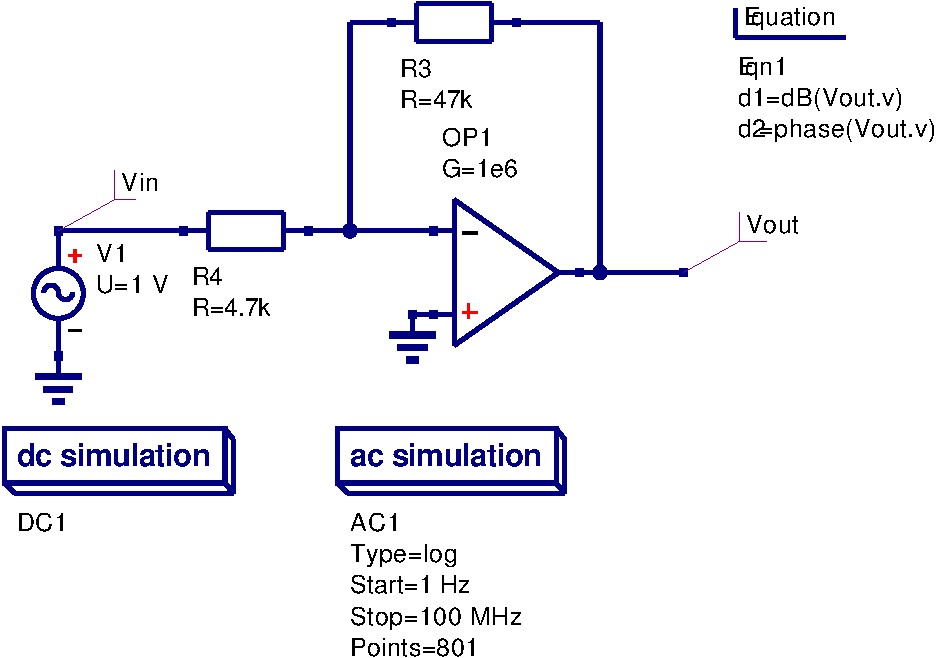
\includegraphics[width=0.9\linewidth]{fig1_sch}
  \caption{Qucs schematic for a basic OP AMP inverting amplifier:Qucs OP AMP has G=1e6 and Umax=15V.}
  \label{fig:opamp1}
\end{figure} 

\begin{figure}
  \centering
  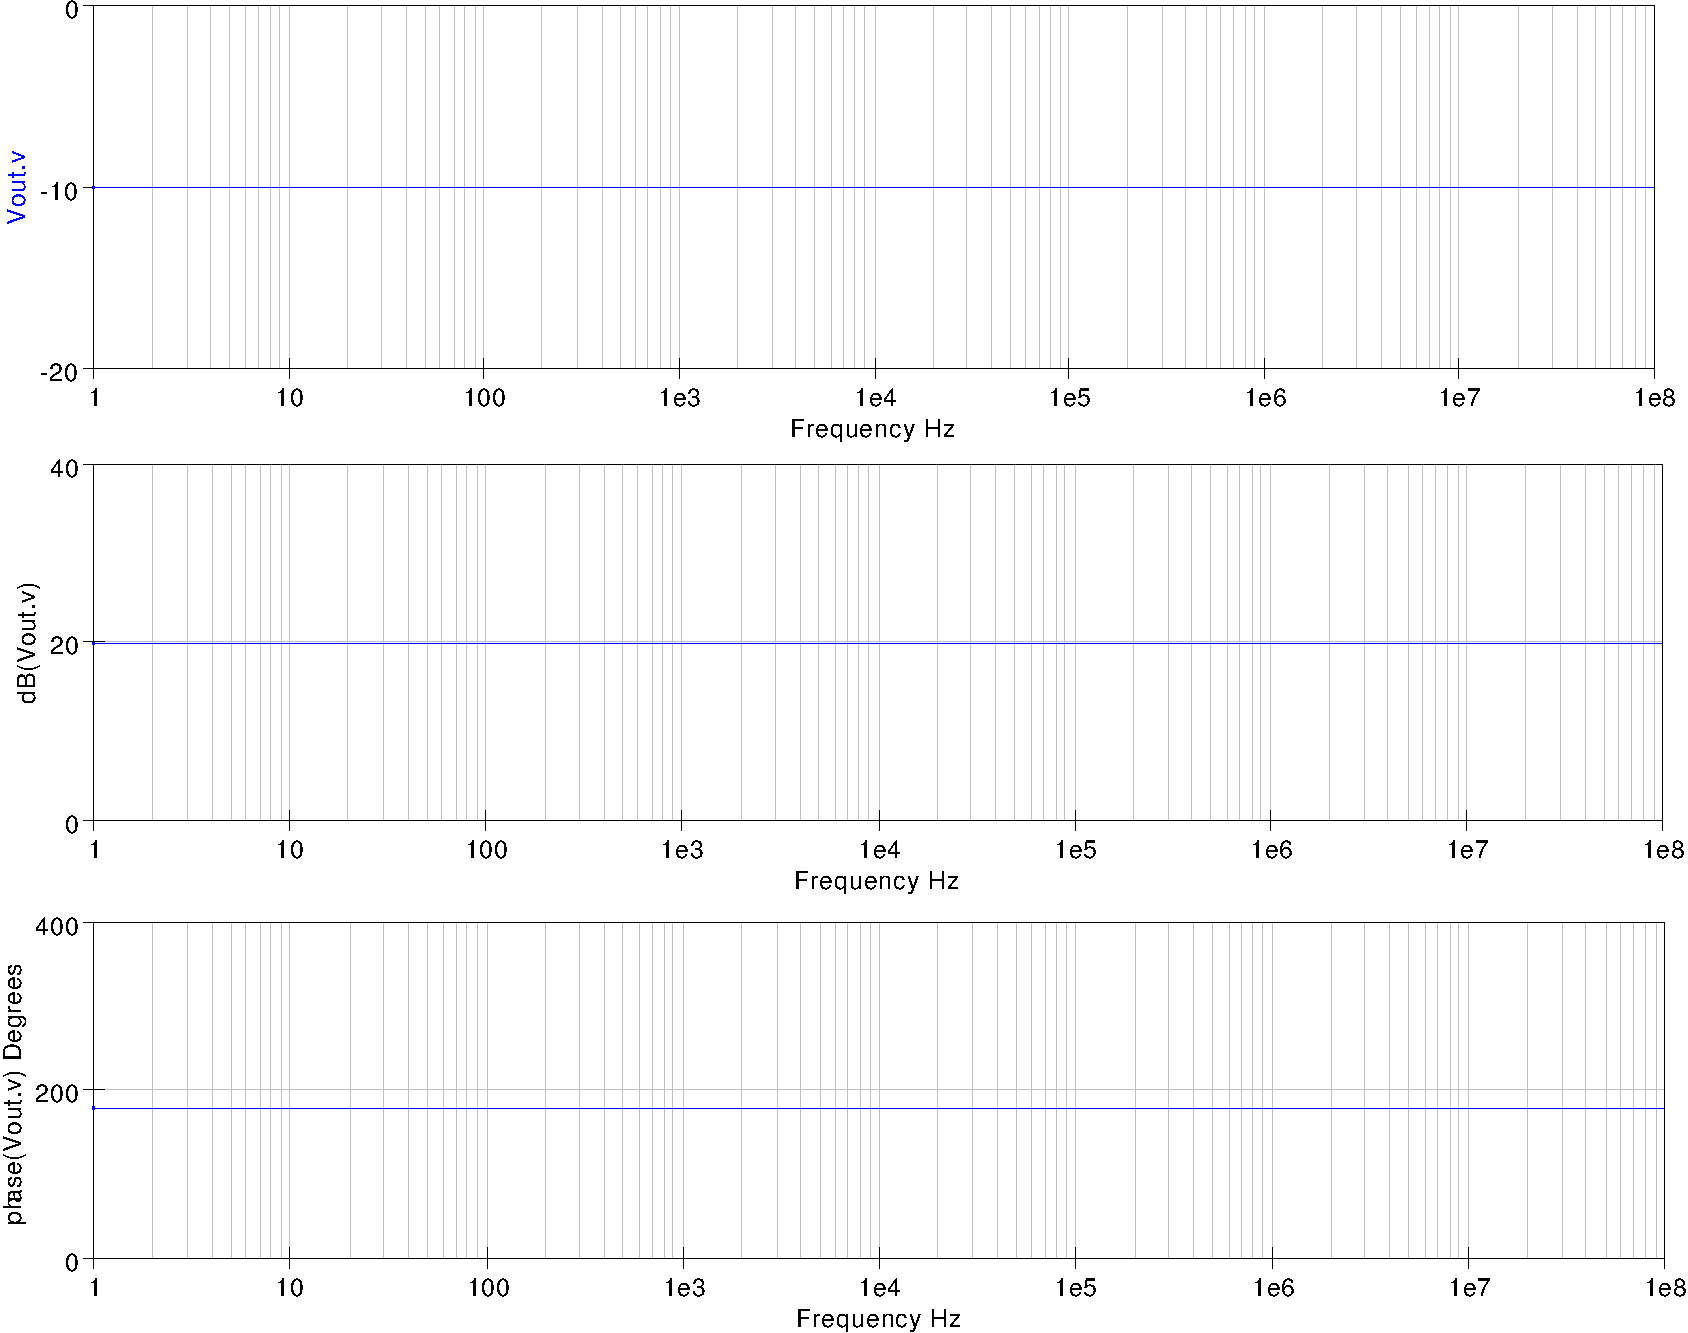
\includegraphics[width=0.9\linewidth]{fig1_dpl}
  \caption{Gain and phase curves for a basic OP AMP inverting amplifier.}
  \label{fig:opamp2}
\end{figure} 

\begin{figure}
  \centering
  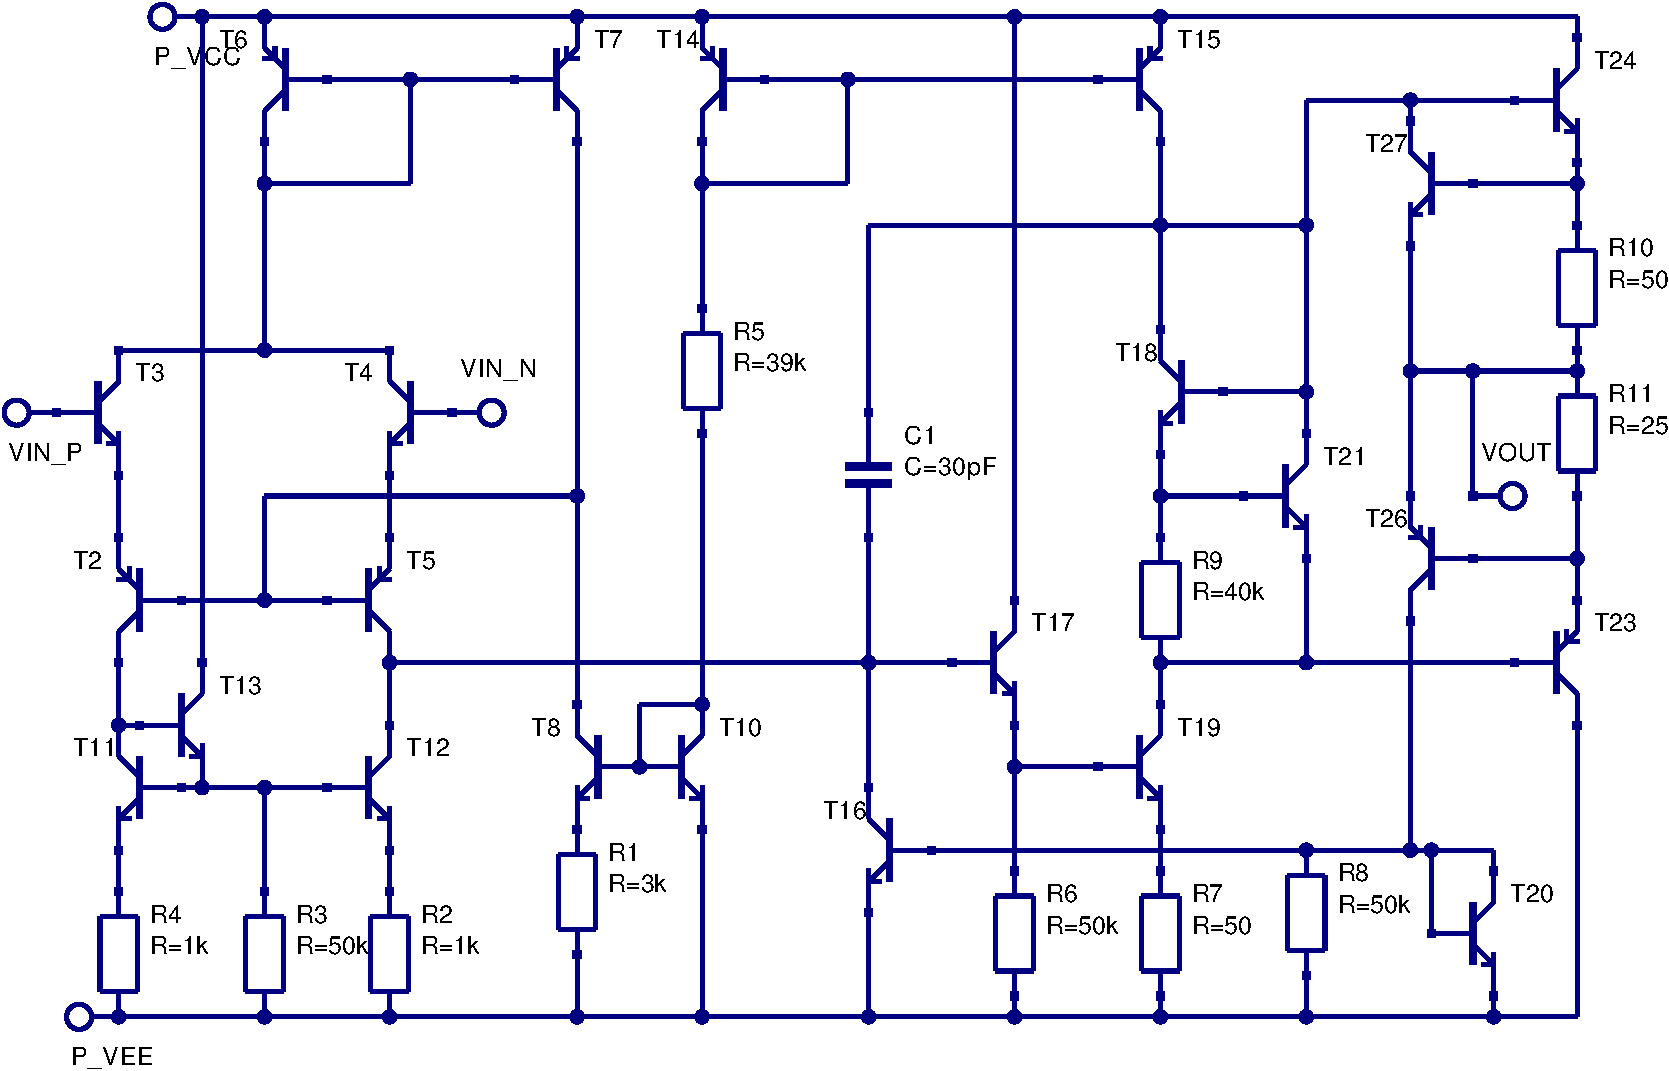
\includegraphics[width=0.9\linewidth]{fig2_sch}
  \caption{Transistor level circuit for the UA741 operational amplifier.}
  \label{fig:opamp3}
\end{figure} 


\begin{figure}
  \centering
  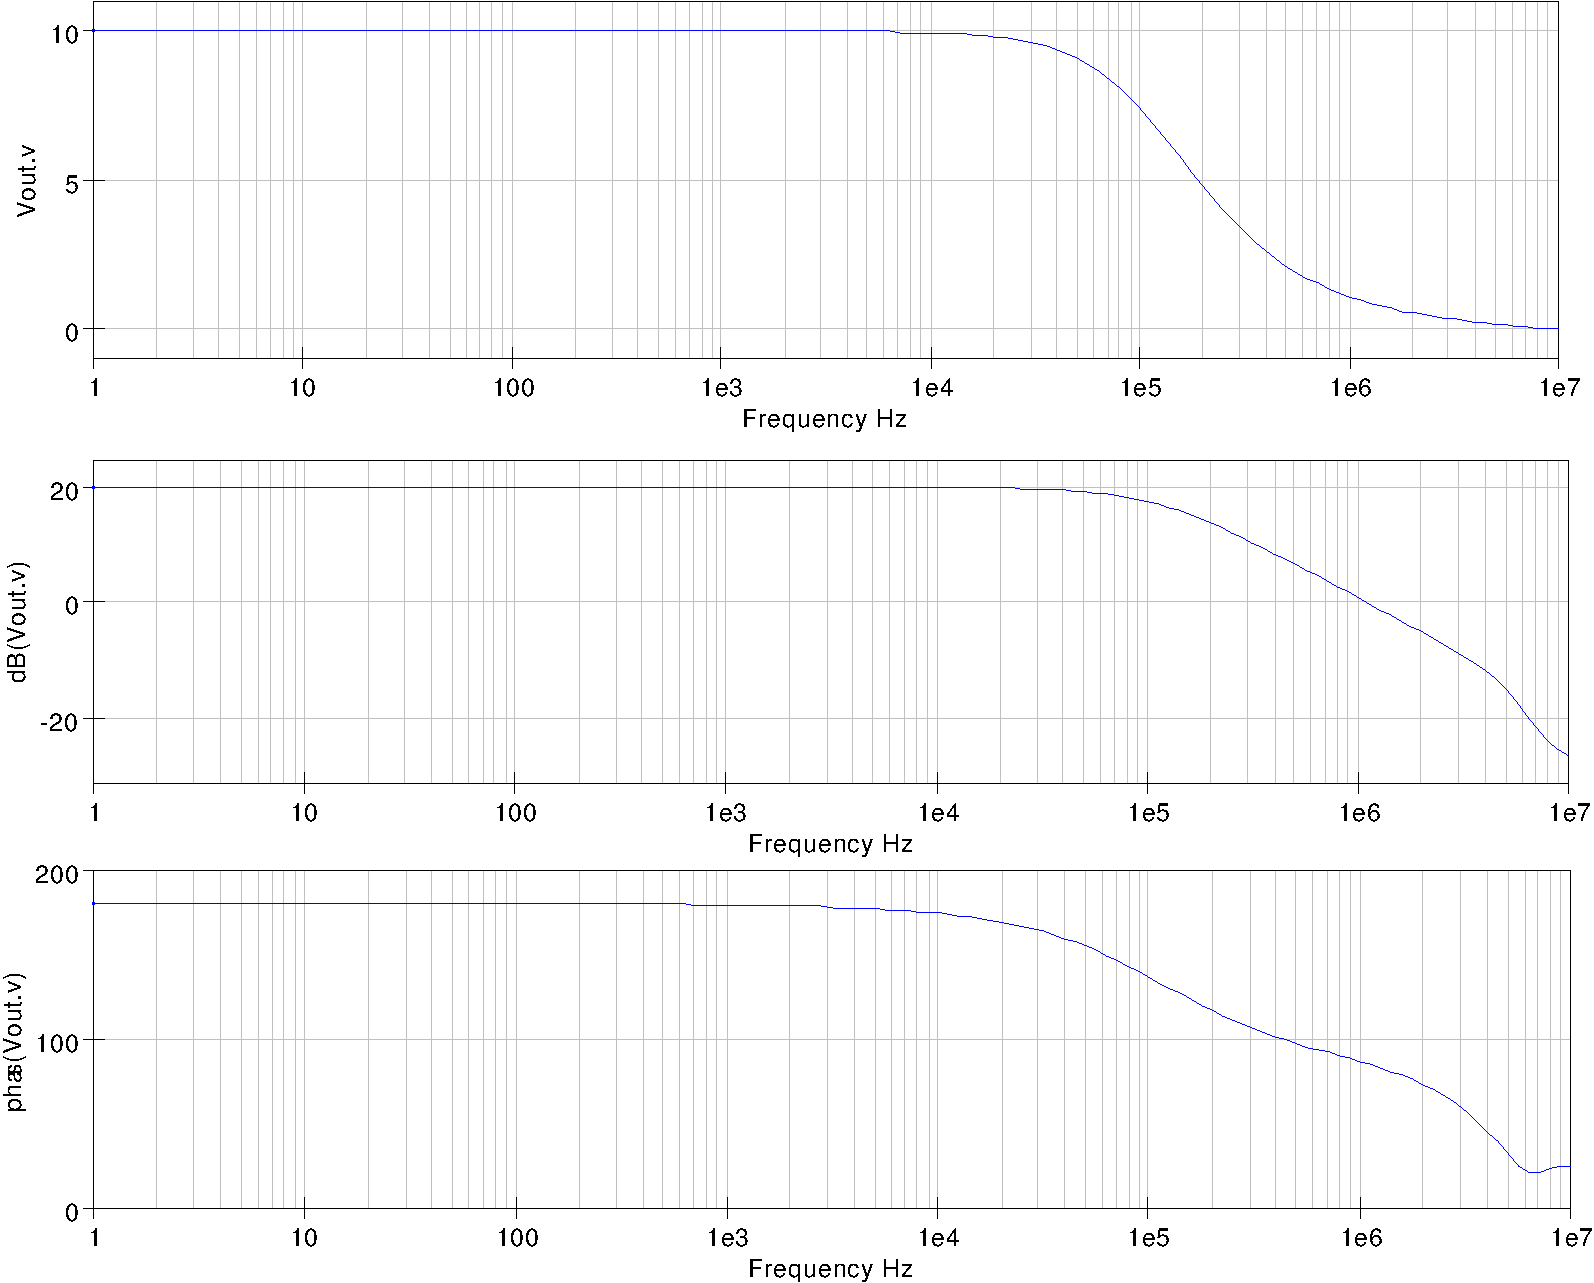
\includegraphics[width=0.9\linewidth]{fig2_dpl}
  \caption{Gain and phase curves for a times 10 inverting amplifier with the OP AMP represented by a transistor level UA741 model.}
  \label{fig:opamp4}
\end{figure} 


\begin{figure}
  \centering
  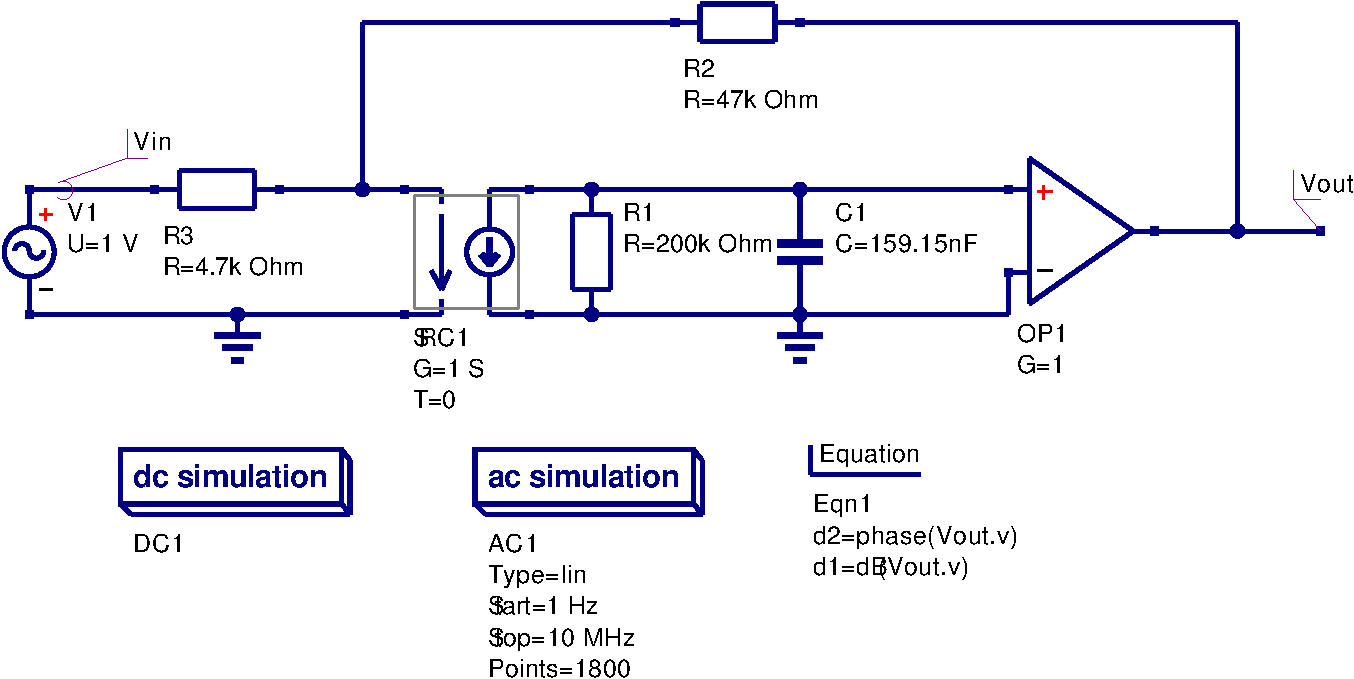
\includegraphics[width=0.9\linewidth]{fig3_sch}
  \caption{Modified Qucs OP AMP model to include single pole frequency response.}
  \label{fig:opamp5}
\end{figure} 

\begin{figure}
  \centering
  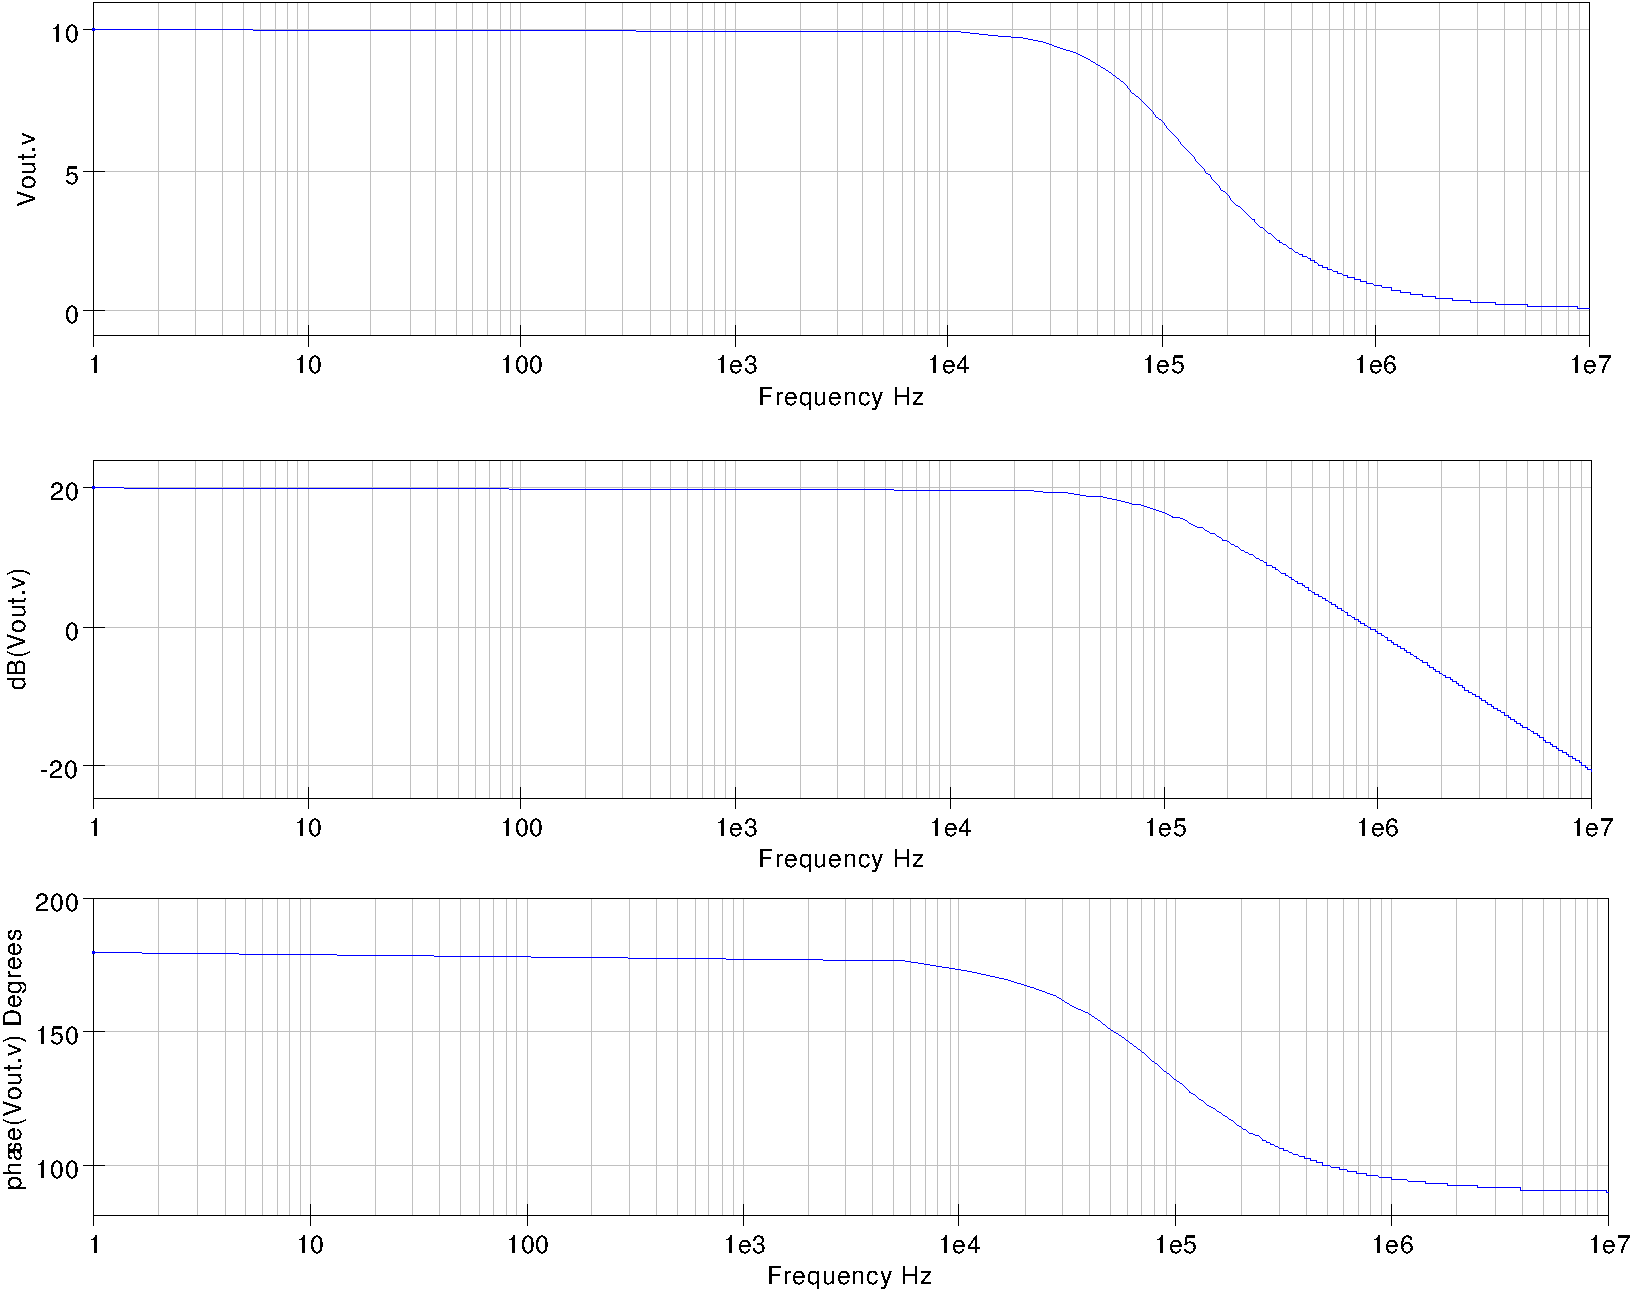
\includegraphics[width=0.9\linewidth]{fig3_dpl}
  \caption{Gain and phase curves for the circuit shown in Fig.~\ref{fig:opamp5}.}
  \label{fig:opamp6}
\end{figure} 

\tutsection{Adding features to the Qucs OP AMP model}

In the previous section it was shown that the Qucs OP AMP model had a frequency response that is independent of frequency.  By adding external components to the Qucs OP AMP model the functionality of the model can be improved.  The UA741 differential open loop gain has a pole at roughly 5Hz and a frequency response that decreases at 20 dB per frequency decade from the first pole frequency up to a second pole frequency at roughly 3 MHz. The circuit shown in Fig.~\ref{fig:opamp5} models the differential frequency characteristics of a UA741 from DC to around 1 MHz. Figure ~\ref{fig:opamp6} illustrates the closed loop frequency response for the modified Qucs OP AMP model.



\tutsection{Modular operational amplifier macromodels}

Macromodelling is a term given to the process of modelling an electronic device as a "black box" where individual device characteristics are specified in terms of the signals, and other properties, observed at the input and output terminals of the black box.  Such models operate at a functional level rather than at the more detailed transistor circuit level, offering considerable gain in computational efficiency.\footnote{  Computational efficiency is increased mainly due to the fact that operational amplifier macromodels have, on average, about one sixth of the number of nodes and branches when compared to a transistor level model.  Furthermore, the number of non-linear p-n junctions included in  a macromodel is often less than ten which compares favorable with the forty to fifty needed to model an amplifier at transistor level.}  Macromodels are normally derived directly from manufacturers data sheets.  For the majority of operational amplifiers, transistor level models are not normally provided by manufacturers.  One notable exception being the UA741 operational amplifier shown in Fig.~\ref{fig:opamp3}.\\
A block diagram of a modular\footnote{Brinson M. E. and Faulkner D. J., Modular SPICE macromodel for operational amplifiers, IEE Proc.-Circuits Devices Syst., Vol. 141, No. 5, October 1994, pp. 417-420.} general purpose OP AMP macromodel is illustrated in Fig.~\ref{fig:opamp7}.  In this diagram the blocks represent specific amplifier characteristics modelled by electrical networks composed of components found in all the popular circuit simulators\footnote{Models employing non-linear controlled sources, for example the SPICE B voltage and current sources, are not allowed in Qucs release 0.0.9. Non-linear controlled sources are one of the features on the Qucs to-do list.}. Each block consists of one or more components which model a single amplifier parameter or a group of related parameters such as the input offset current and voltage.  This ensures that changes to one particular parameter do not indirectly change other parameters.  Local nodes and scaling are also employed in the macromodel blocks.  Furthermore, because each block operates separately, scaled voltages do not propagate outside individual blocks. Each block can be modelled with a Qucs subcircuit that has the required specification and buffering from other blocks.  Moreover, all subcircuits are self contained entities where the internal circuit details are hidden from other blocks.  Such an approach is similar to structured high-level computer programming where the internal details of functions are hidden from users.   Since the device characteristics specified by each block are separate from all other device characteristics only those amplifier characteristics which are needed are included in a given macromodel. This approach leads to a genuinely structured macromodel.  The following sections present the detail and derivation of the electrical networks forming the blocks drawn in Fig.~\ref{fig:opamp7}. To illustrate the operation of the modular OP AMP macromodel the values of the block parameters are calculated for the UA741 OP AMP and used in a series of example simulations.  Towards the end of this tutorial note data are presented for a number of other popular general purpose operational amplifiers.
\tutsection{A basic AC OP AMP macromodel. }

A minimum set of blocks is required for the modular macromodel to function as an amplifier: an input stage, a gain stage and an output stage.  These form the core modules of all macromodels.  

\tutsubsection{The input stage.}
The input stage includes amplifier offset voltage, bias and offset currents, and the differential input impedance components. The circuit for the input stage is shown in Fig.~\ref{fig:opamp8}, where
\begin{enumerate}
\item \textit{R1   = R2} = Half of the amplifier differential input resistance (\textit{RD}).
\item \textit{Cin}   = The amplifier differential input capacitance (\textit{CD}).
\item \textit{Ib1    = Ib2} = The amplifier input bias current (\textit{IB}).
\item \textit{Ioff}  = Half the amplifier input offset current (\textit{IOFF}).
\item \textit{Voff1 = Voff2} = Half the input offset voltage ( \textit{VOFF}).
\end{enumerate}

Typical values for the UA741 OP AMP are:

\begin{enumerate}
\item \textit{RD} = 2 M$\Omega$ and \textit{R1 = R2} = 1M$\Omega$
\item \textit{CD} = \textit{Cin1} = 1.4 pF.
\item \textit{IB} = \textit{Ib1} = \textit{Ib2 }= 80 nA.
\item \textit{IOFF} = 20 nA and \textit{Ioff1} = 10 nA.
\item \textit{VOFF} = 0.7 mV and \textit{Voff1 = Voff2} = 0.35 mV.
\end{enumerate}

\FloatBarrier
\begin{figure}
  \centering
  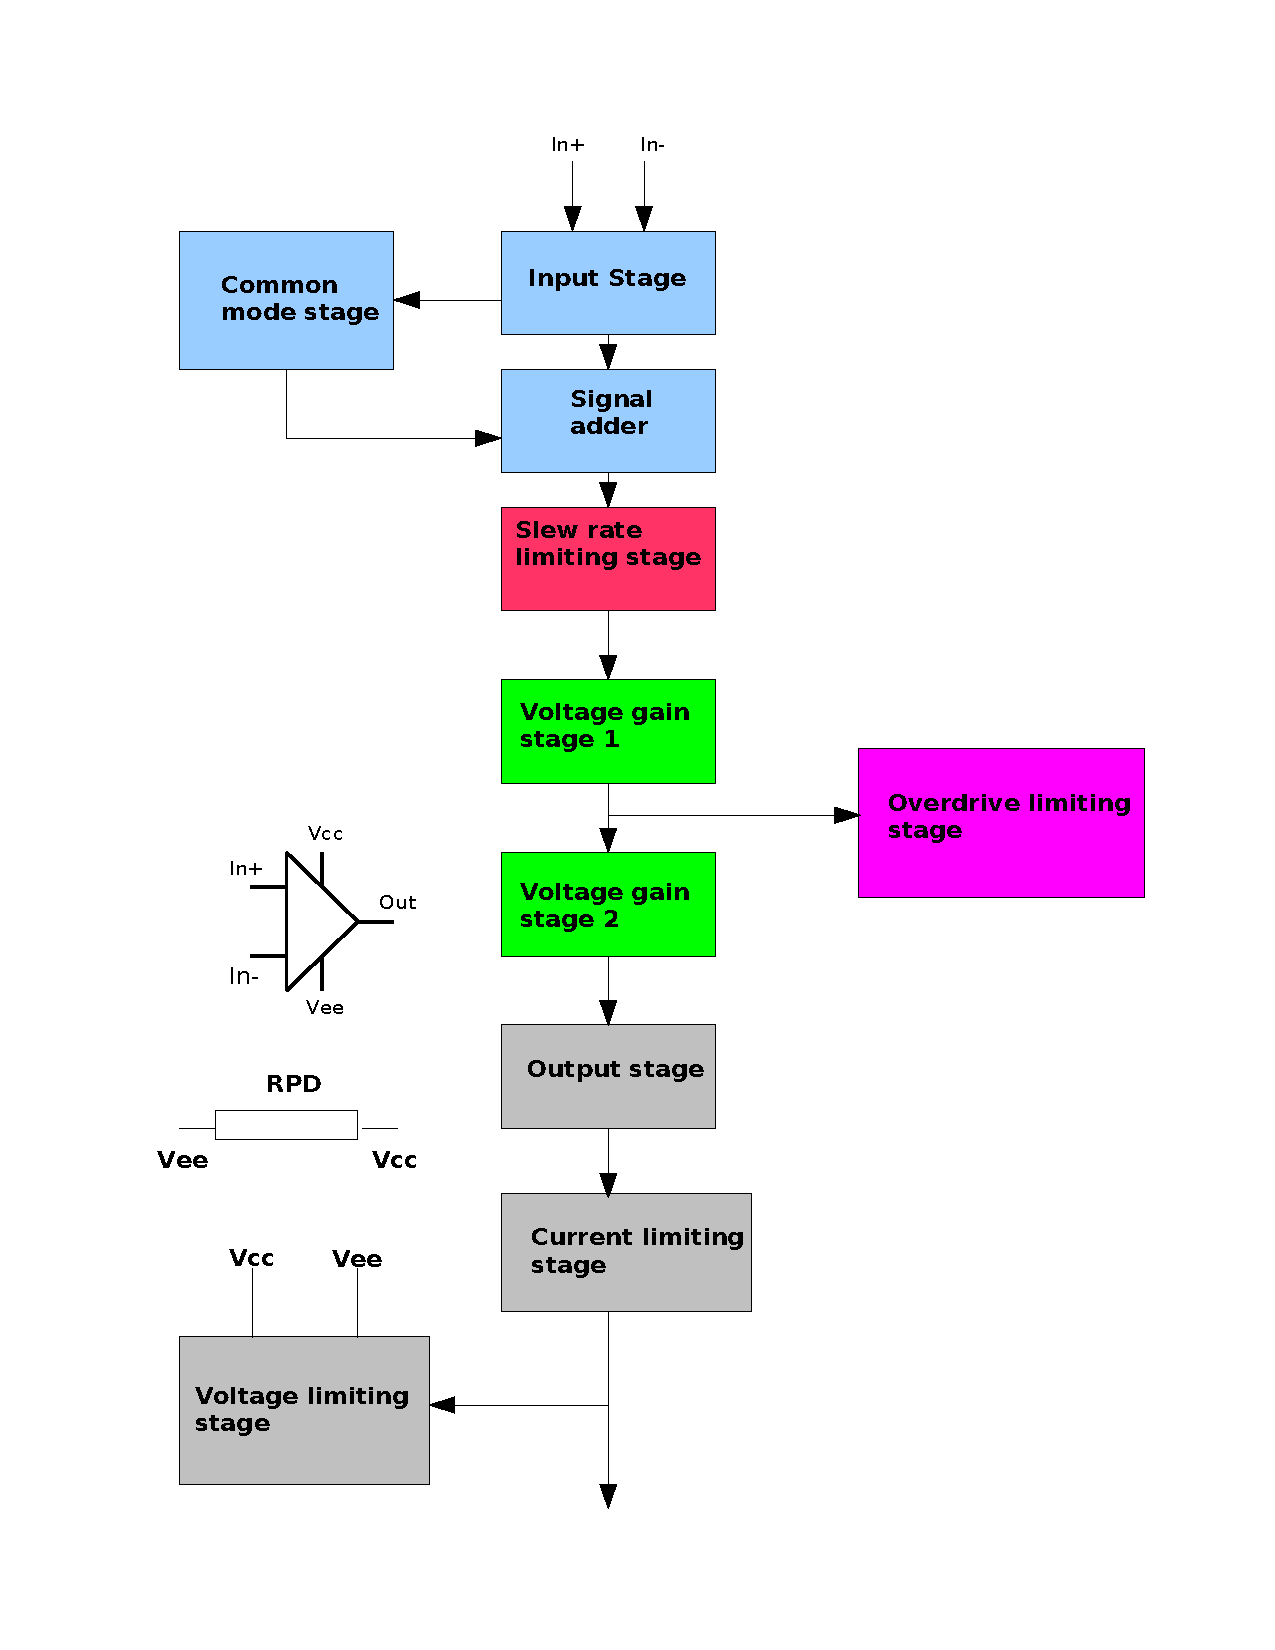
\includegraphics[width=1.0\linewidth]{dwr1}
  \caption{Block diagram of an operational amplifier macromodel.} 
  \label{fig:opamp7}
\end{figure} 
\FloatBarrier


The differential output signal (VD) is given by $VD_{-}P1 - VD_{-}N1$ and the common mode output signal (\textit{VCM}) by $(VD_{-}P1 + VD_{-}N1)/2$.
\FloatBarrier
\begin{figure}
  \centering
  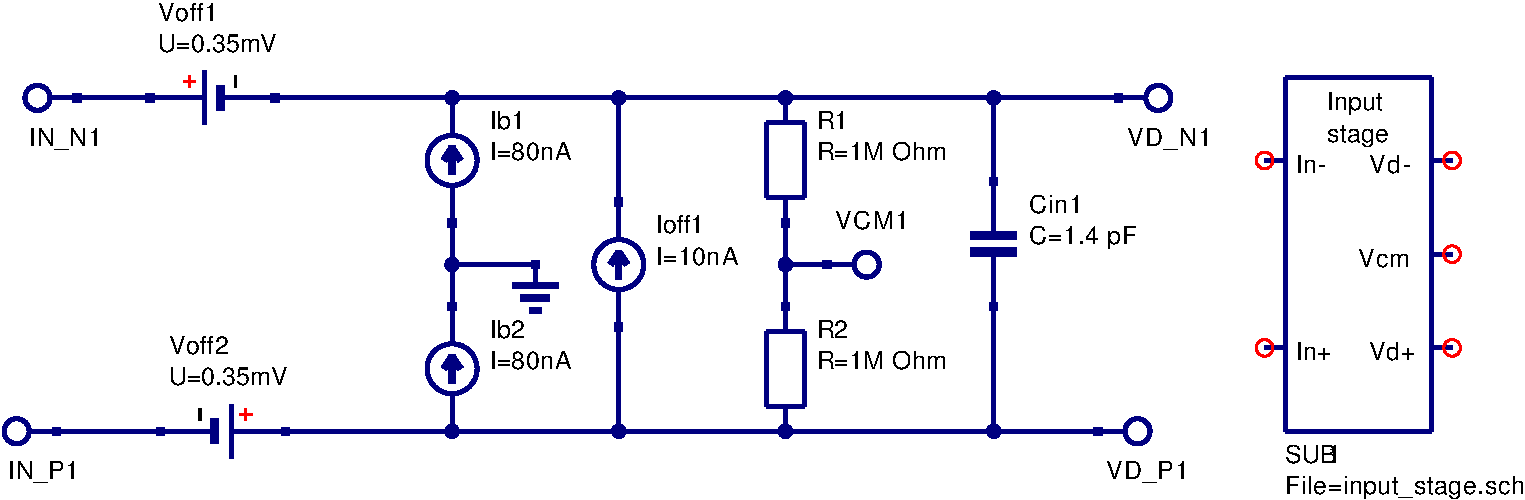
\includegraphics[width=1.0\linewidth]{fig8_sch}
% tcomb1.png: 99.9998dpi, width=11.35cm, height=3.35cm, bb=0 0 447 132
  \caption{Modular OP AMP input stage block.}
  \label{fig:opamp8}
\end{figure}
\FloatBarrier

\tutsubsection{Voltage gain stage 1.}
The circuit for voltage gain stage 1 is shown in Fig.~\ref{fig:opamp9}, where
\begin{enumerate}
\item\textit{ RD1} = 100 M$\Omega$ = A dummy input resistor - added to ensure nodes $IN_{-}P1$ and $IN_{-}N1$ are connected by a DC path.
\item \textit{GMP1} = 1 S = Unity gain voltage controlled current generator.
\item \textit{RADO }= The DC open loop differential gain ( \textit{AOL(DC)} ) of the OP AMP.
\item \textit{CP1}  = \textit{1/(2*$\pi$*GBP)}, where \textit{GBP} = the OP AMP gain bandwidth product.
\end{enumerate}

Typical values for the UA741 OP AMP are:
\begin{enumerate}
\item \textit{RADO} =  200k$\Omega$. ($AOL(DC)$ = 106 dB)
\item \textit{CP1}  =  159.15 nF  (The typical value for UA741 GBP is 1 MHz).
\end{enumerate}



\FloatBarrier
\begin{figure}
  \centering
  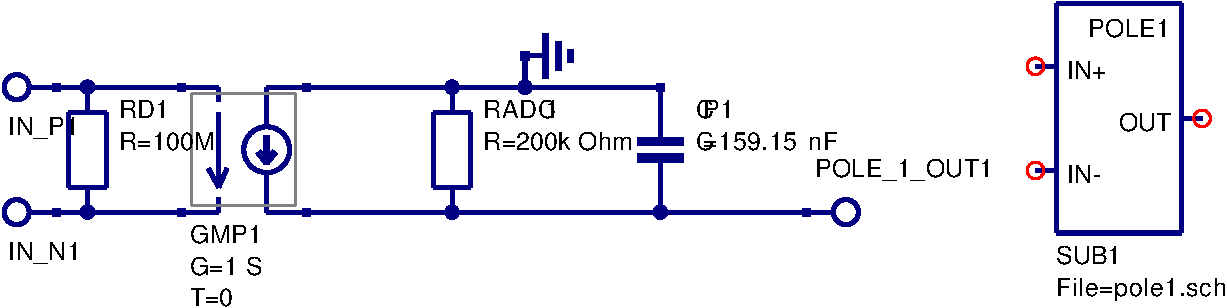
\includegraphics[width=1.0\linewidth]{fig9_sch}
% tcomb1.png: 99.9998dpi, width=11.35cm, height=3.35cm, bb=0 0 447 132
  \caption{Modular OP AMP first voltage gain stage.}
  \label{fig:opamp9}
\end{figure}



\tutsubsection{Derivation of voltage gain stage 1 transfer function}

Most general purpose operational amplifiers have an open loop differential voltage gain which has (1) a very high value at DC (2) a dominant pole (\textit{fp1}) at a low frequency - typically below 100 Hz, and (3) a gain response characteristic that rolls-off at 20 dB per decade up to a unity gain frequency which is often in the MHz region.  This form of response has a constant gain bandwidth product (\textit{GBP}) over the frequency range from \textit{fp1} to \textit{GBP}.  A typical OP AMP differential open loop response is shown in Fig.~\ref{fig:opamp10}. The voltage gain transfer function for this type of characteristic can be modelled with the electrical network given in Fig.~\ref{fig:opamp9}, where the the AC voltage transfer function is


\begin{equation}
vout(POLE_{-}1_{-}OUT1) = \dfrac{ GMP1 * ( V( IN _{-} P1 ) - V(IN _{-} N1) ) * RADO} { 1 + j (\omega * RADO * CP1 ) }
\end{equation}
Where \begin{equation}
        f_{P1} = \dfrac {1} {2\pi * RADO * CP1}
      \end{equation}
Let \textit{RADC = Aol(DC)} and \textit{GMP1 = 1 S}. Then, because \textit{fp1*AOL(DC) = GBP},
\begin{equation} 
CP1 = \dfrac{1} { 2\pi*GBP}
\end{equation}

\begin{figure}
  \centering
  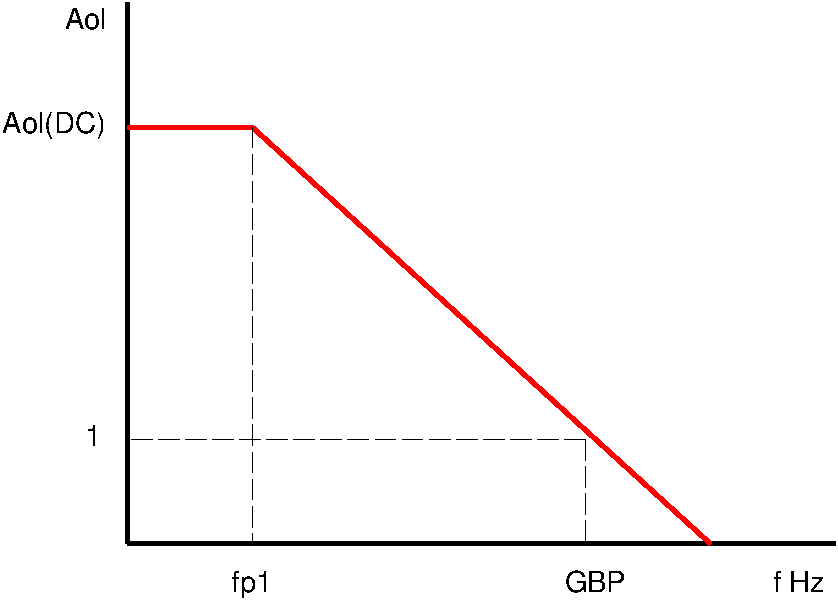
\includegraphics[width=0.8\linewidth]{fig10_diag}
% tcomb1.png: 99.9998dpi, width=11.35cm, height=3.35cm, bb=0 0 447 132
  \caption{OP AMP open loop differential voltage gain as a function of frequency.}
  \label{fig:opamp10}
\end{figure}

\newpage 

\tutsubsection{Output stage.}
The electrical network representing a basic output stage is given in Fig.~\ref{fig:opamp11}, where

\begin{enumerate}
\item \textit{ RD1}     = 100 M$\Omega$ = A dummy input resistor - added to ensure nodes $IN_{-}P1$ and $IN_{-}N1$ are connected by a DC path.
\item \textit{EOS1}   G = 1 = Unity gain voltage controlled voltage generator.
\item \textit{ROS1}     =  OP AMP output resistance.
\end{enumerate}

A typical value for the UA741 OP AMP output resistance is \textit{ROS1} =  75$\Omega$.


\begin{figure}
  \centering
  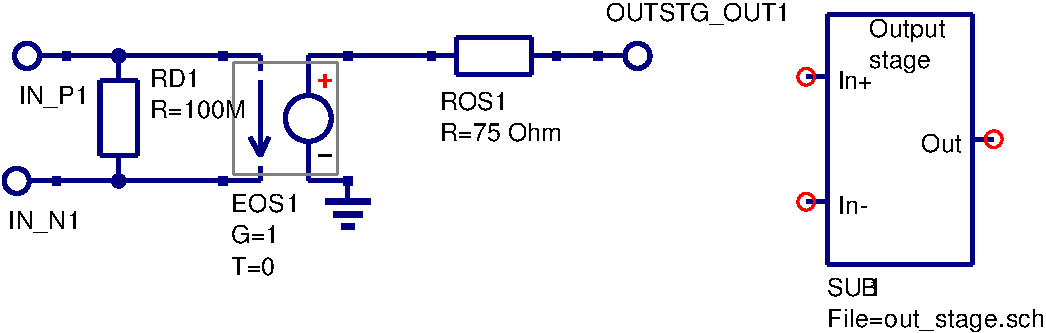
\includegraphics[width=0.8\linewidth]{fig11_sch}
% tcomb1.png: 99.9998dpi, width=11.35cm, height=3.35cm, bb=0 0 447 132
  \caption{Modular macromodel output stage.}
  \label{fig:opamp11}
\end{figure}

\tutsubsection{A subcircuit model for the basic AC OP AMP macromodel}
The model for the basic AC OP AMP macromodel is shown in Fig.~\ref{fig:opamp12}. The input stage common mode voltage ($Vcm$) is not used in this macromodel and has been left floating.  To test the performance of the AC macromodel it's operation was compared to the transistor level UA741 model. Figure ~\ref{fig:opamp13} shows a schematic circuit for two inverting amplifiers, each with a gain of ten, driven from a common AC source. One of the amplifiers uses the simple AC macromodel and the other the transistor level UA741 model.  Figure ~\ref{fig:opamp14} illustrates the output gain and phase curves for both amplifiers. In general the plotted curves are very similar.  However, at frequencies above the GBP frequency the basic AC macromodel does not correctly model actual OP AMP performance. This is to be expected because the simple AC macromodel does not include any high frequency modelling components.  Notice also that the DC output voltages for vout and vout3 are very similar, see the DC tabular results given in Fig.~\ref{fig:opamp13}. 

\begin{figure}
  \centering
  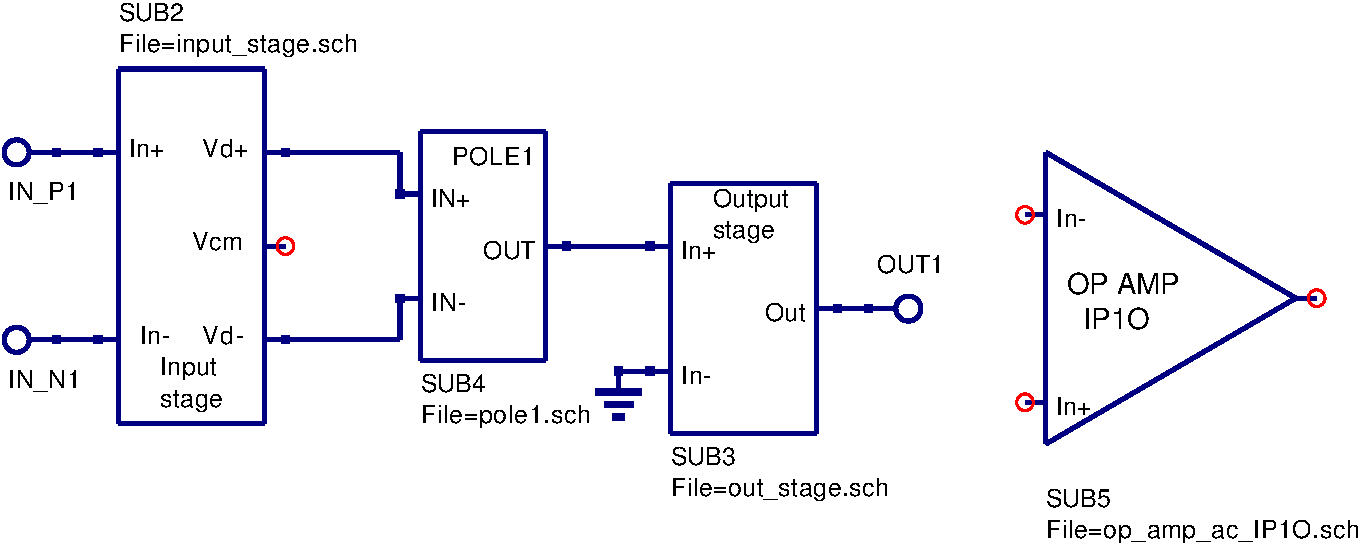
\includegraphics[width=1.0\linewidth]{fig12_sch} 
% tcomb1.png: 99.9998dpi, width=11.35cm, height=3.35cm, bb=0 0 447 132 
  \caption{Simple AC OP AMP macromodel.}
  \label{fig:opamp12}
\end{figure}

\begin{figure}
  \centering
  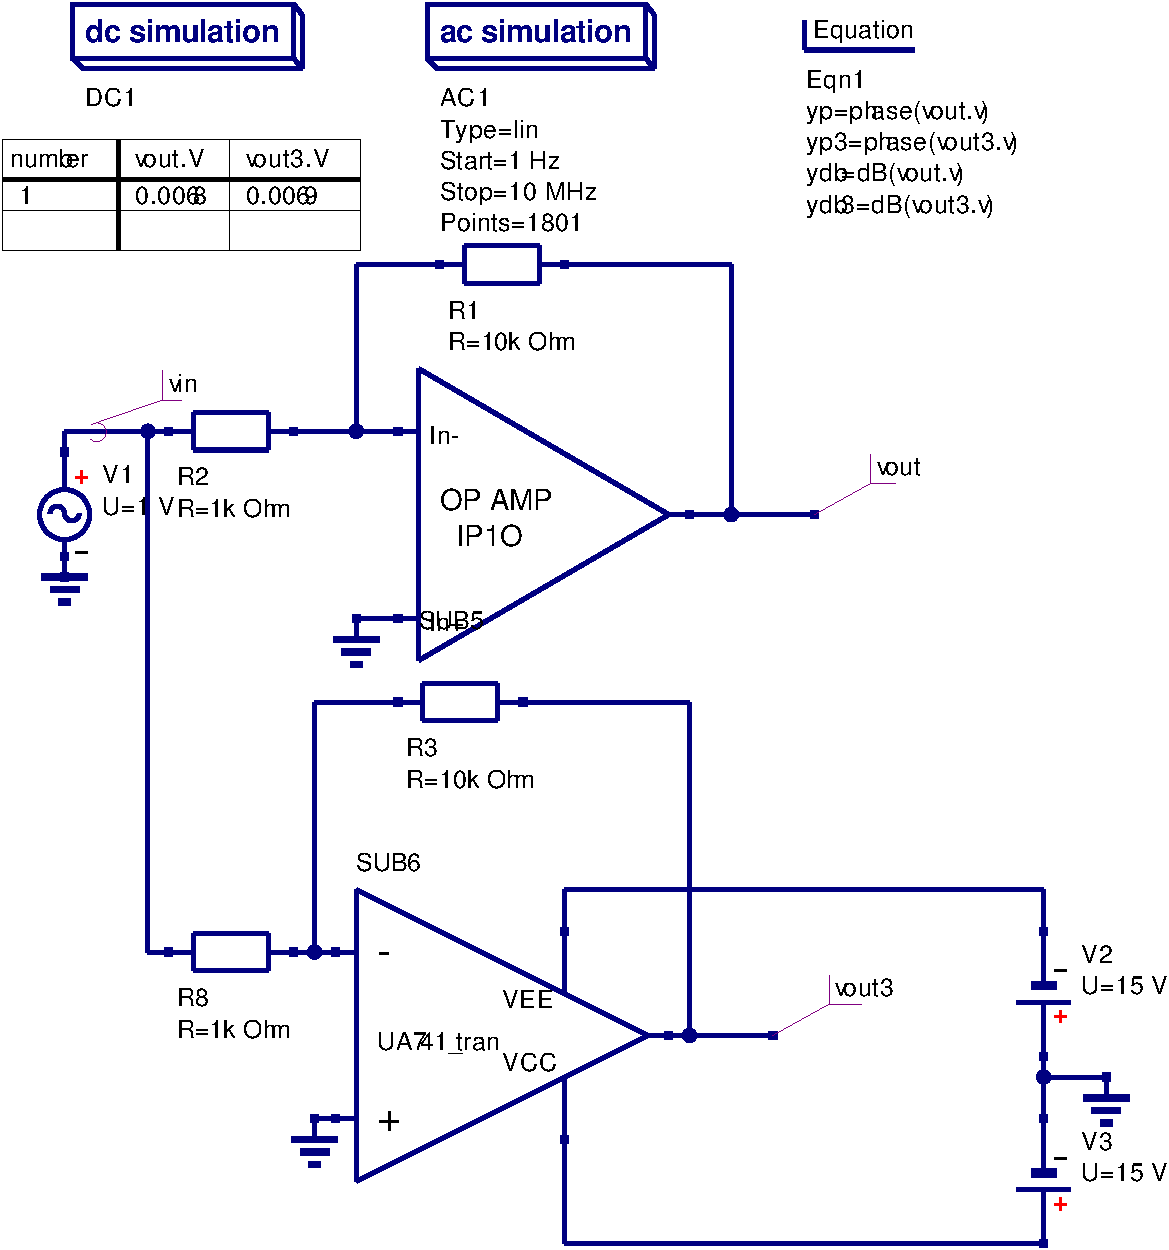
\includegraphics[width=0.9\linewidth]{fig13_sch}
% tcomb1.png: 99.9998dpi, width=11.35cm, height=3.35cm, bb=0 0 447 132
 \caption{Test circuit for an inverting amplifier. Output signals: (1) vout for AC macromodel, (2) vout3 for UA741 transistor model.}
  \label{fig:opamp13}
\end{figure}

\begin{figure}
  \centering
  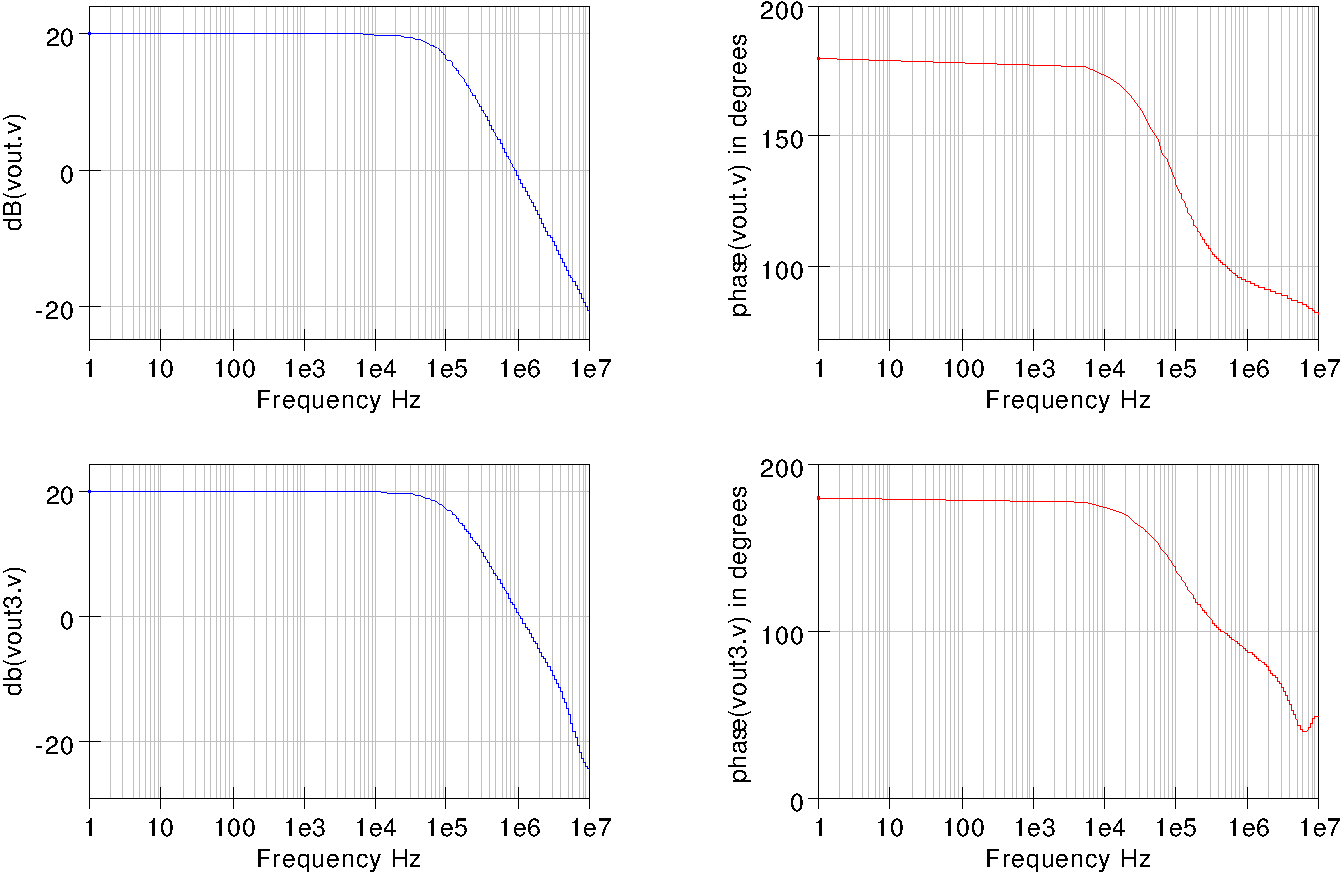
\includegraphics[width=0.9\linewidth]{fig14_dpl}
% tcomb1.png: 99.9998dpi, width=11.35cm, height=3.35cm, bb=0 0 447 132
  \caption{Simulation test results for the circuit shown in Fig.~\ref{fig:opamp13}.} 
  \label{fig:opamp14}
\end{figure}

\tutsection{ A more accurate OP AMP AC macromodel}

Most general purpose OP AMPs have a high frequency pole in their differential open loop gain characteristics.  By adding a second gain stage to the simple AC macromodel the discrepancy in the high frequency response can be corrected.  The model for the second gain stage is shown in Fig.~\ref{fig:opamp15}.  This additional gain stage has a structure similar to the first gain stage, where

\begin{enumerate}
\item\textit{RD2} = 100 M$\Omega$ = A dummy input resistor - added to ensure nodes \verb|IN_P2| and \verb|IN_N2| are connected by a DC path.
\item \textit{GMP2} = 1 S = Unity gain voltage controlled current generator.
\item \textit{RP2 } = 1$\Omega$.
\item \textit{CP2}  = \textit{1/(2$\pi$*fp2)}, where $fp2$ = the second pole frequency in Hz.
\end{enumerate}

A typical value for the UA741 OP AMP high frequency pole is  \textit{fp2}  =  3M Hz 


\begin{figure}
  \centering
  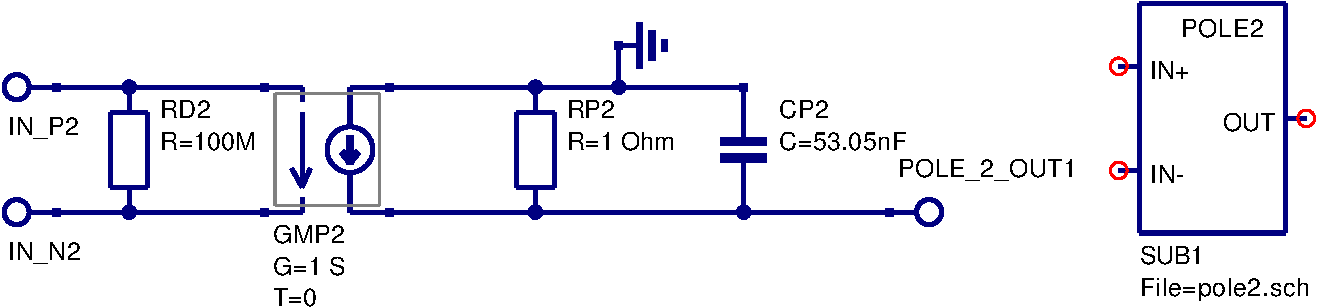
\includegraphics[width=0.9\linewidth]{fig15_sch}
% tcomb1.png: 99.9998dpi, width=11.35cm, height=3.35cm, bb=0 0 447 132
  \caption{Modular OP AMP second voltage gain stage.}
  \label{fig:opamp15}
\end{figure}

\tutsubsection{Derivation of voltage gain stage 2 transfer function.}
The differential voltage gain transfer function for voltage gain stage 2 is given by

\begin{equation}
vout(POLE_{-}2_{-}OUT1) = \dfrac{ GMP2 * ( V( IN _{-} P2 ) - V(IN _{-} N2) ) * RP2} { 1 + j (\omega * RP2 * CP2 ) }
\end{equation}

Let \textit{RP2 = 1$\Omega$} and \textit{GMP2 = 1 S}. Then 

\begin{equation}
vout(POLE_{-}2_{-}OUT1) = \dfrac{ V( IN _{-} P2 ) - V(IN _{-} N2)} { 1 + j (\omega *  CP2 ) }
\end{equation}

and

\begin{equation} 
CP2 = \dfrac{1} { 2\pi*fp2}
\end{equation}

\newpage
\tutsubsection{Simulating OP AMP open loop differential gain}

The circuit shown in Fig.~\ref{fig:opamp16} allows the open loop differential gain \textit{(Aol(f))} to be simulated. This circuit employes a feedback resistor to ensure DC stability.  Fig.~\ref{fig:opamp16} illustrates two test circuits driven from a common AC source. This allows the performance of the AC macromodel and the UA741 transistor level model to be compared. The AC voltage transfer function for the test circuit is
  
\begin{equation}
vout(f) = \dfrac{ Aol(f)} { 1 +  \dfrac{ Aol(f) }{1 + j \omega * R * C} } vin(f)
\end{equation} 

where $vout(f) = (V^{+} - V^{-})*Aol(f)$,  $V^{+} = vin(f)$, and $V^{-} = \dfrac{vout(f)}{1 + j \omega * R * C} $

Provided $\dfrac{Aol(f)}{\omega*R*C} << 1$, equation (7) becomes $vout(f) \Rightarrow Aol(f) * vin(f)$. Hence, for those frequencies where this condition applies \textit{vout(f) = Aol(f)} when\textit{ vin(f)} = 1 V.  Figure 17 shows plots of the open loop simulation data. Clearly with the test circuit time constant set at 1e6 seconds the data is accurate for frequencies down to 1 Hz. 


\begin{figure}
  \centering
  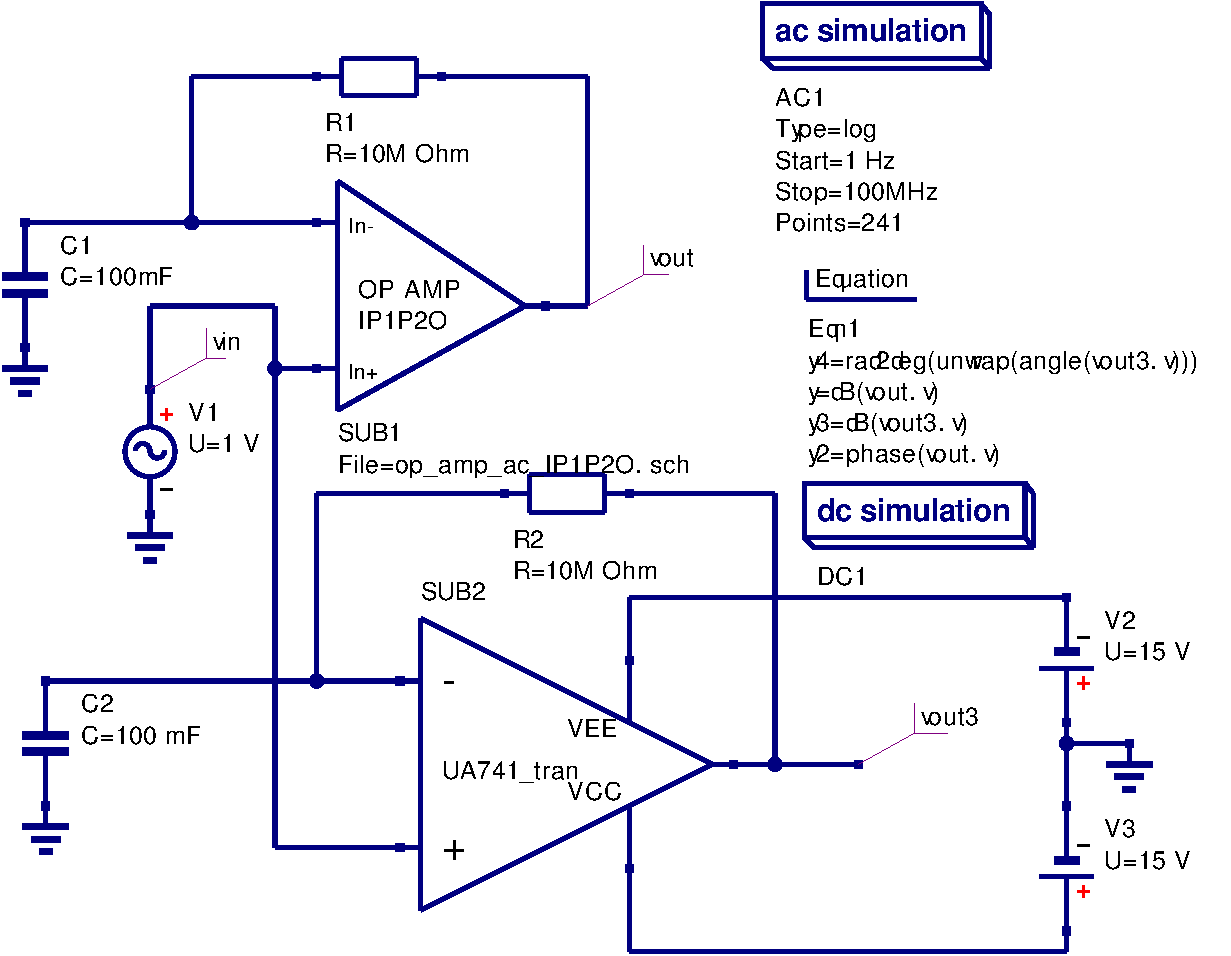
\includegraphics[width=0.8\linewidth]{fig16_sch}
% tcomb1.png: 99.9998dpi, width=11.35cm, height=3.35cm, bb=0 0 447 132
  \caption{Test circuit for simulating OP AMP open loop differential gain.}  
  \label{fig:opamp16}
\end{figure}

\begin{figure}
  \centering
  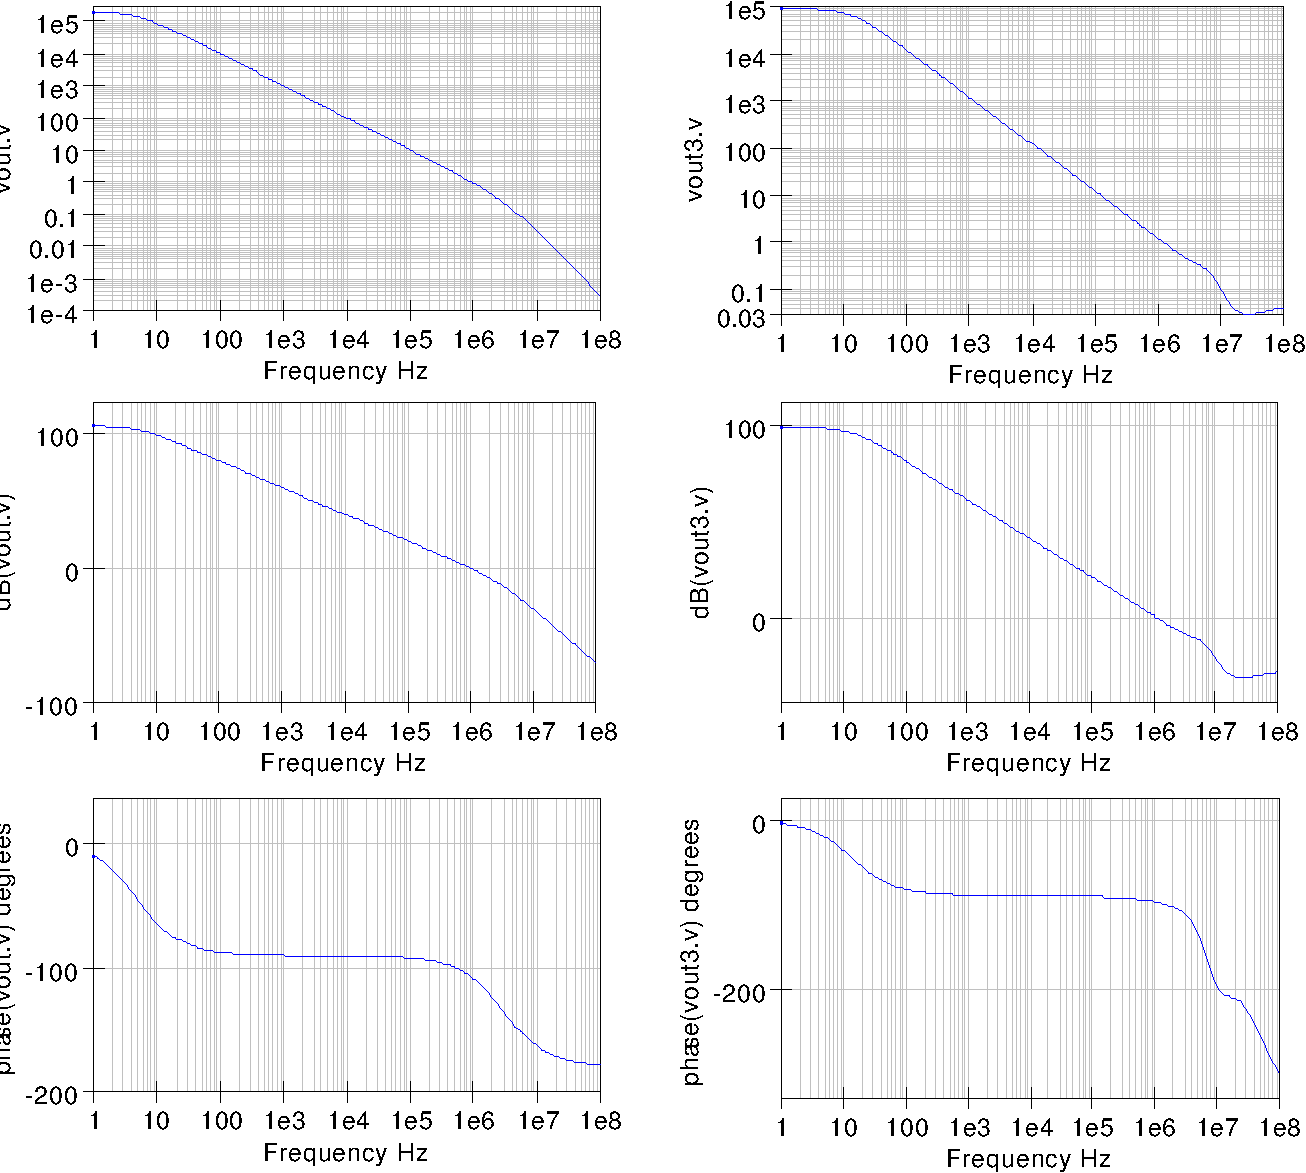
\includegraphics[width=0.9\linewidth]{fig17_dpl}
% tcomb1.png: 99.9998dpi, width=11.35cm, height=3.35cm, bb=0 0 447 132
  \caption{Simulation test results for the circuit shown in Fig.~\ref{fig:opamp16}.}
  \label{fig:opamp17}
\end{figure}

\tutsection{Adding common mode effects to the OP AMP AC macromodel}

The open-loop differential gain $A_{D}(f)$ for most general purpose operational amplifiers can be approximated by

\begin{equation}
A_{D}(f)=AD(0)\dfrac{1}{1+j\dfrac{f}{f_{PD}}}
\end{equation}

Similarly, the common-mode gain $A_{CM}(f)$ can be represented by the same single-pole response and a single zero response given by
\begin{equation}
A_{CM}(f)=A_{CM}(0)\dfrac{1+j\dfrac{f}{f_{CMZ}}}{1+j\dfrac{f}{f_{PD}}}
\end{equation}
Defining the common-mode rejection ratio $CMRR(f)$ of an OP AMP as
\begin{equation}
CMRR(f)=\dfrac{A_{D}(f)}{A_{CM}(f)}
\end{equation}

gives
\begin{equation}
CMRR(f)=CMRR(0)\dfrac{1}{1+j\dfrac{f}{f_{CMZ}}}
\end{equation}
where
\begin{equation}
CMRR(0)=\dfrac{A_{D}(0)}{A_{CM}(0)}
\end{equation}

Common-mode effects can be added to OP AMP macromodels by including a stage in the modular macromodel that introduces a zero in the amplifier frequency response.  Output $V_{CM}$ from the macromodel input stage senses an amplifier common mode signal.  This signal, when passed through a CR network generates the required common mode zero. Figure 18 gives the model of the zero generating network, where.

\begin{enumerate}
\item \textit{RDCMZ} = 650 M$\Omega$ = common-mode input resistance/2.
\item \textit{RCM1 } = 1 M$\Omega$
\item \textit{ECM1}    G = 31.623 = $\dfrac{\dfrac{RCM1}{RCM2}}{CMRR(0)}$. (NOTE: \textit{RCM1/RCM2}is a scaling factor.)
\item \textit{CCM1}  = 795.8 pF = $\dfrac{1}{2\pi*RCM1*f_{CMZ}}$.
\item \textit{RCM2 } = 1 $\Omega$
\end{enumerate}
Typical values for the UA741 OP AMP are:
\begin{enumerate}
\item Common-mode input resistance = 1300 M$\Omega$.
\item \textit{CMRR(0)} =  90 dB 
\item \textit{$f_{CMZ}$} =  200 Hz.
\end{enumerate}


\begin{figure}
  \centering
  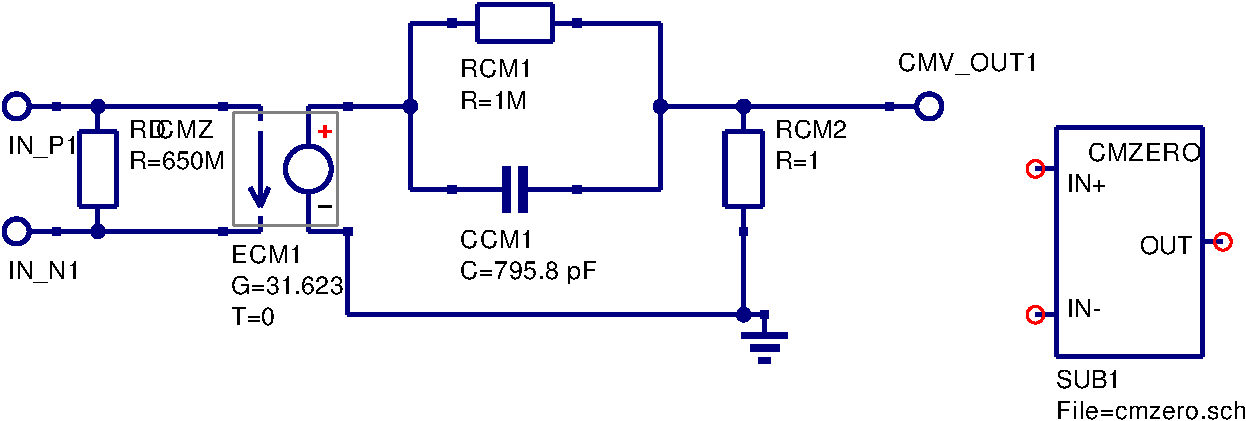
\includegraphics[width=0.9\linewidth]{fig18a_sch}
% tcomb1.png: 99.9998dpi, width=11.35cm, height=3.35cm, bb=0 0 447 132
  \caption{Common-mode zero macromodel}
  \label{fig:opamp18a}
\end{figure}

The AC voltage transfer function for the common-mode zero transfer function is

\begin{equation}
Vout(\verb|CMV_OUT1|)=G(ECM1)\dfrac{RCM2}{RCM1}\left[  \dfrac{1+j\omega*RCM1*CCM1}{1+j\omega*RCM2*CCM1}\right] \left[ V(\verb|IN_P1|)-V(\verb|IN_N1|)\right] 
\end{equation}

As $\dfrac{RCM2}{RCM1} << 1$, the pole introduced by the common-mode RC network is at a very high frequency and can be neglected. Combining the common-mode zero with the previously defined stage models yields the macromodel shown in Fig.~\ref{fig:opamp18b}.  In this model the differential and common-mode signals are combined using a simple analogue adder based on voltage conrolled current generators.

\begin{figure}
  \centering
  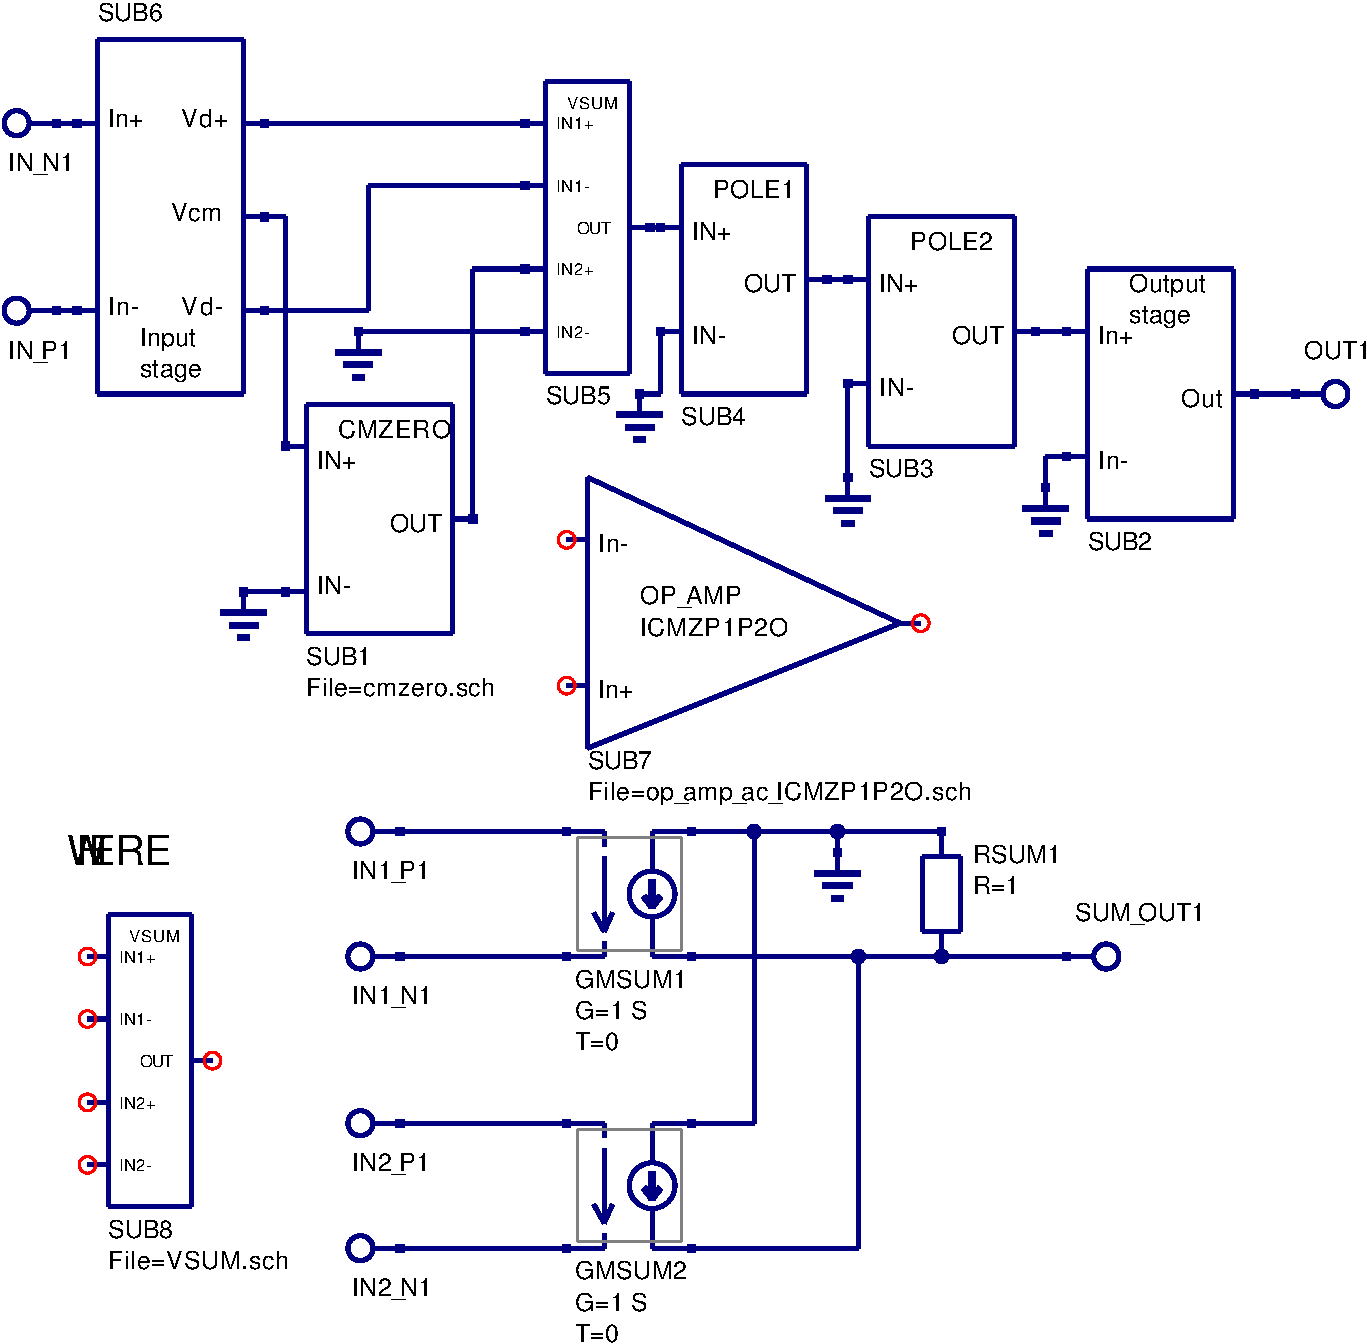
\includegraphics[width=0.9\linewidth]{fig18b_sch}
% tcomb1.png: 99.9998dpi, width=11.35cm, height=3.35cm, bb=0 0 447 132
  \caption{AC macromodel including common-mode zero.}
  \label{fig:opamp18b}
\end{figure}

\tutsubsection{Simulating OP AMP common-mode effects}
OP AMP common-mode effects can be simulated using the circuit shown in Fig.~\ref{fig:opamp20}.\footnote{Brinson M.E. and Faulkner D.J., New approaches to measurement of operational amplifier common-mode rejection ratio in the frequency domain, IEE Proc-Circuits Devices Sys., Vol 142, NO. 4, August 1995, pp 247-253.} The resulting output voltages (vout.v and vout3.v) for a test circuit with matched resistors are shown plotted in Fig.~\ref{fig:opamp21}, where
$\dfrac{vout(0)}{vin}=\dfrac{1}{CMRR(0)}$.  Clearly the test results for the macromodel and the UA741 transistor model are very similar.  In the case of the macromodel typical device parameters were used to calculate the macromodel component values.  However, in the transistor level model the exact values of the component parameters are unknown.\footnote{The UA741 transistor level model is based on an estimate of the process parameters that determine the UA741 transistor characteristics.  Hence, the device level model is unlikely to be absolutely identical to the model derived from typical parameters values found on OP AMP data sheets. From the simulation results the CMRR(0) values are approximately (1) macromodel 90 dB, (2) UA741 transistor model 101 dB. Similarly, the common-mode zero frequencies are approximately (1) macromodel 200 Hz, (2) UA741 transistor model 500 Hz.}

\begin{figure}
  \centering
  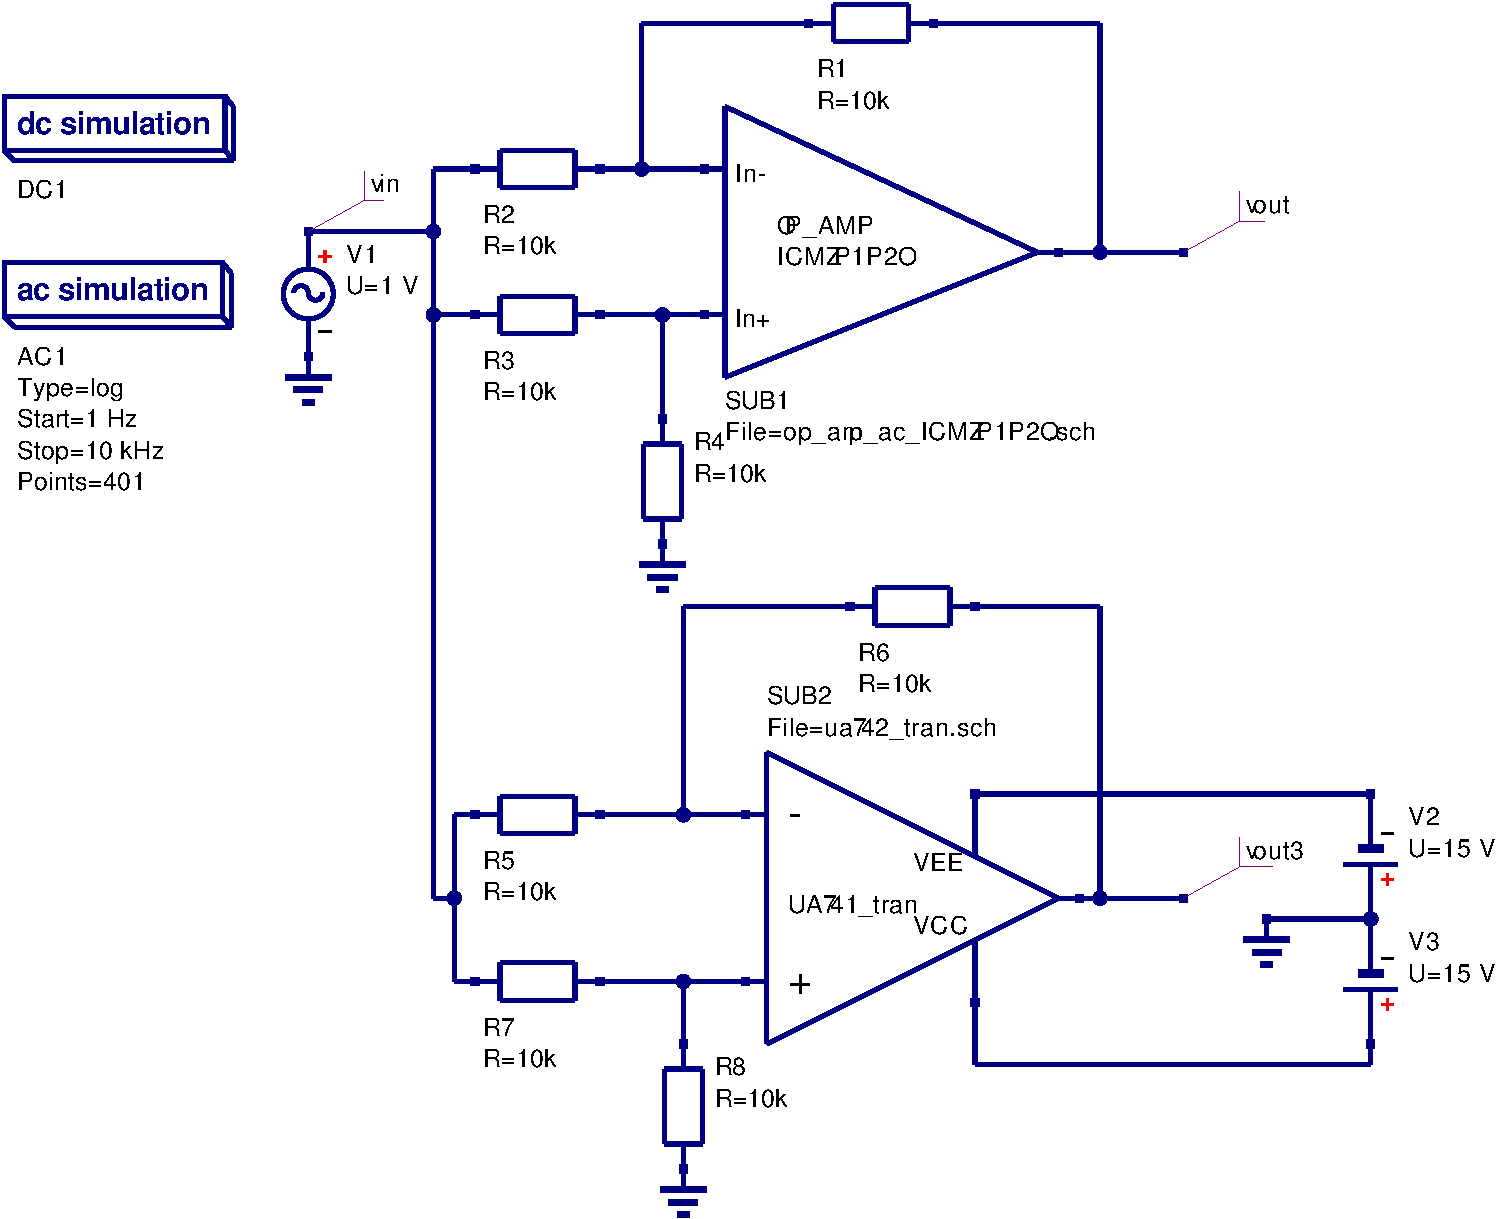
\includegraphics[width=0.9\linewidth]{fig20_sch}
% tcomb1.png: 99.9998dpi, width=11.35cm, height=3.35cm, bb=0 0 447 132
  \caption{Simulation of OP AMP common-mode performance.}
  \label{fig:opamp20}
\end{figure}

\begin{figure}
  \centering
  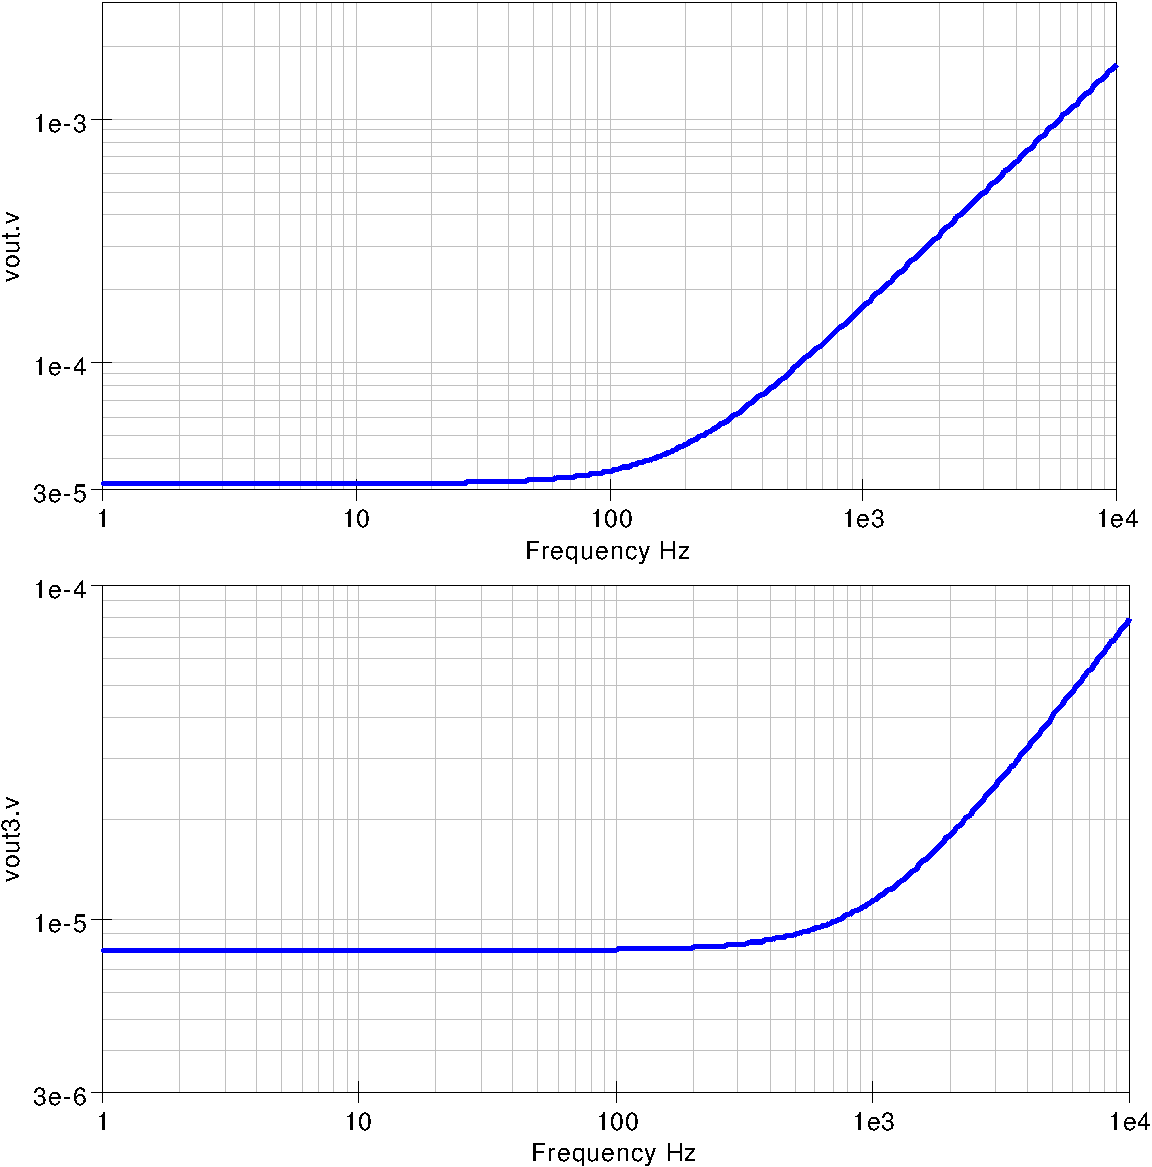
\includegraphics[width=0.9\linewidth]{fig20_dpl}
% tcomb1.png: 99.9998dpi, width=11.35cm, height=3.35cm, bb=0 0 447 132
  \caption{Simulation test results for the circuit shown in Fig.~\ref{fig:opamp20}.}
  \label{fig:opamp21}
\end{figure}



\tutsection{Large signal transient domain OP AMP macromodels}

The modular macromodel introduced in the previous sections concentrated on modelling OP AMP performance in the small signal AC domain. Large signal models need to take into account the passage of signals through an OP AMP in the time domain and limit the excursion of voltage and current swings to the practical values found in actual amplifiers. Starting with the AC domain macromodel introduced in the previous sections, adding a slew rate limiting stage and a overdrive stage will more correctly model OP AMP high speed large signal limitations. Furthermore, by adding output voltage and current limiting stages the OP AMP macromodel will correctly model large signal effects when signal levels approach circuit power supply voltages or the OP AMP output current limits. 

\tutsubsection{Slew rate macromodel derivation}

The slew rate of an OP AMP can be modelled by limiting the current charging $CP1$ in the first voltage gain stage POLE1. From Fig.~\ref{fig:opamp9}

\begin{equation}
GMP1 \left(  V(IN_{-}P1) - V(IN_{-}N1) \right)  = \dfrac{ V( POLE_{-}1_{-}OUT1 ) } {RADO}+CP1*\dfrac{ dV(POLE_{-}1_{-}OUT1) } {dt} 
\end{equation}

Hence, provided $RADO$ is large\footnote{This condition is normally true because $RADO$ is set to the DC open loop differential gain in macromodule POLE1. }

\begin{equation}
GMP1 \left(  V( IN_{-}P1 ) - V( IN_{-}N1 ) \right)  \simeq  CP1*\dfrac{ dV(POLE_{-}1_{-}OUT1) } {dt}  
\end{equation}


But $ CP1 = \dfrac{1}{2\pi*GBP}$ 


Yielding

\begin{equation}
GMP1 \left(  V(IN_{-}P1) - V(IN_{-}N1) \right)  \simeq \dfrac{1}{2\pi*GBP}*\dfrac{ dV(POLE_{-}1_{-}OUT1) } {dt}  
\end{equation}

Moreover, if $\dfrac{ dV(POLE_{-}1_{-}OUT1)}{dt}$ is set equal to the OP-AMP slew rate then the current\\
 
charging \textit{CP1} will be limited to the maximum allowed. In Fig.~\ref{fig:opamp9} $GMP1$ is 1 S. \\

Therefore, voltage difference  $ V(IN_{-}P1) - V(IN_{-}N1)$\\

must be set to $\dfrac{1}{2\pi*GBP}*\dfrac{ dV(POLE_{-}1_{-}OUT1) } {dt}$.\\

This is done by the network SLEWRT shown in Fig.~\ref{fig:opamp22}, where

\begin{figure}
  \centering
  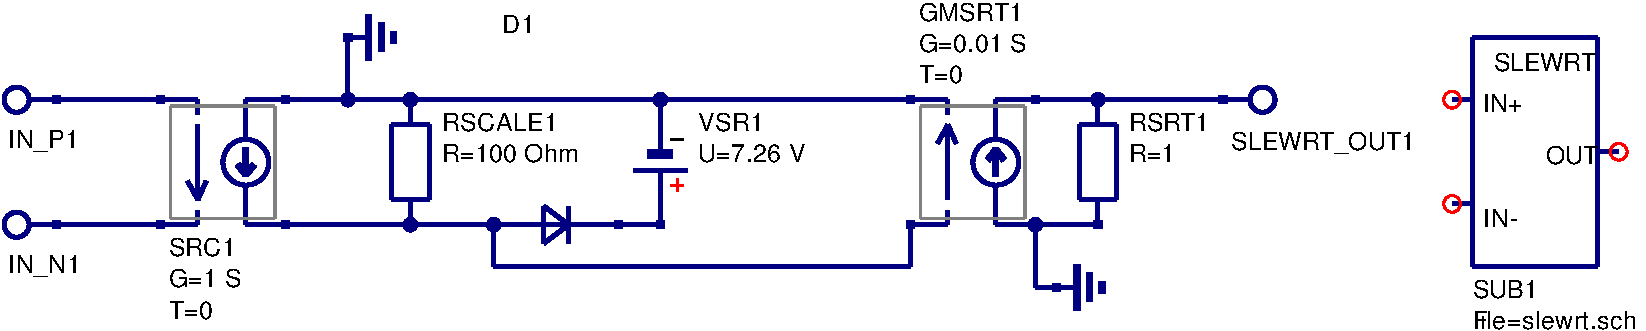
\includegraphics[width=0.9\linewidth]{fig22_sch}
% tcomb1.png: 99.9998dpi, width=11.35cm, height=3.35cm, bb=0 0 447 132
  \caption{OP AMP slew rate macromodel.}
  \label{fig:opamp22}
\end{figure}

\begin{enumerate}
\item \textit{RSCALE1}  = 100 $\Omega$ = Scaling resistance (Scale factor x 100).
\item \textit{SRC1}   G = 1 S.
\item \textit{VSR1}    = V1.
\item \textit{GMSRT1}  G = 0.01 S. (Scale factor = 1/100).
\item \textit{RSRT1}    = 1 $\Omega$
\end{enumerate}
And, 
\begin{enumerate}
\item $V1 = \dfrac{100 * Positive_{-}slew_{-}rate}{2\pi*GBP}-0.7V$
\item $V2 = \dfrac{100 * Negative_{-}slew_{-}rate}{2\pi*GBP}-0.7V$
\item The diode parameters are IS=1e-12 IBV=20mA BV=V1+V2, others default.
\end{enumerate}

Typical values for the UA741 OP AMP are:
\begin{enumerate}
\item $Positive_{-}slew_{-}rate$ = $Negative_{-}slew_{-}rate$ = 0.5V/$\mu$S.
\item $V1$ = $V2$ = 7.25V.
\end{enumerate}

Scaling is used in the slew rate model to allow the use of higher voltages in the clamping circuit. Increased voltages reduce errors due to the forward biased junction voltage. Current limiting results by clamping the voltage across resistor $RSCALE1$ with a diode. This diode acts as a zener diode and saves one nonlinear junction when compared to conventional clamping circuits.  The output section of the SLEWRT circuit removes the internal scaling yielding an overall gain of unity for the module.\\


The circuit in Fig.~\ref{fig:opamp23} demonstrates the effect of slew rate limiting on OP AMP transient performance. Three identical OP AMP inverter circuits are driven from a common input 10 kHz AC signal source. Voltage controlled voltage sources are used to amplify the input signal to the second and third circuits.  The three input signals are (1) 5 V peak, (2) 10 V peak and (3) 15 V peak respectively.  The input and output waveforms for this circuit are illustrated in Fig.~\ref{fig:opamp24}. The effect of slew rate limiting on large signal transient performance is clearly demonstrated by these curves. In the case of the 15 V peak input signal the output signal (vout3.Vt) has a slope that is roughly 0.5 V per $\mu$S. 

\begin{figure}
  \centering
  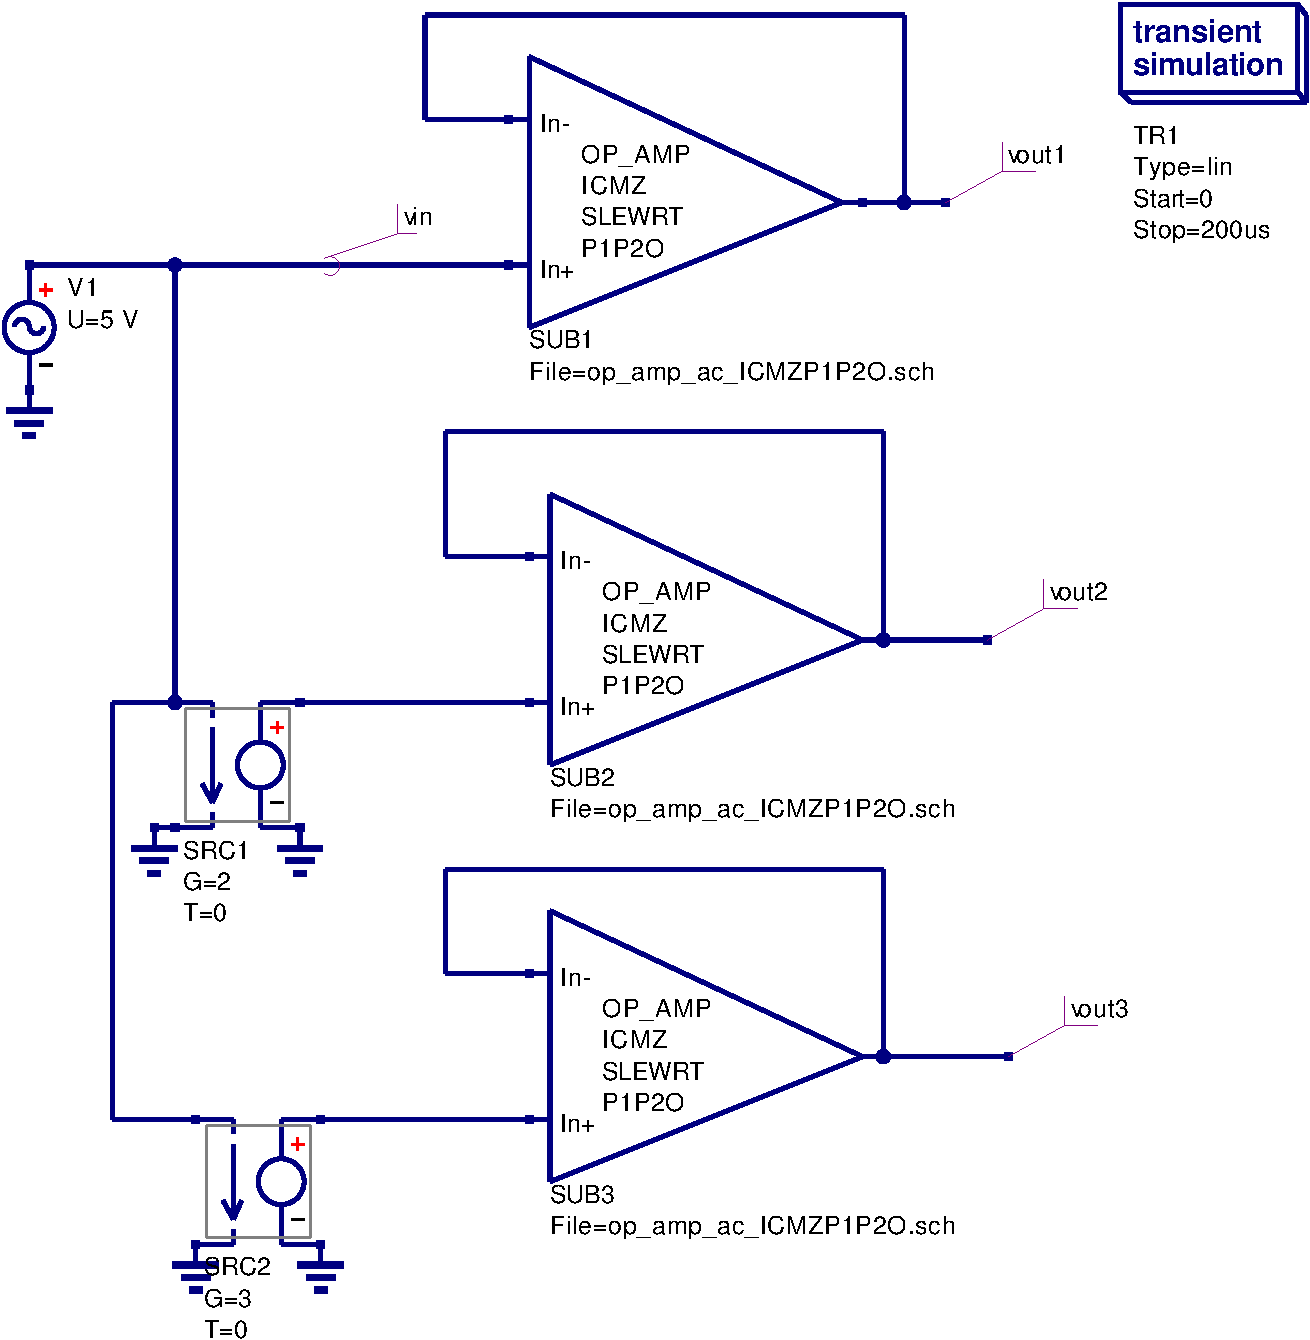
\includegraphics[width=0.9\linewidth]{fig23_sch}
% tcomb1.png: 99.9998dpi, width=11.35cm, height=3.35cm, bb=0 0 447 132
  \caption{OP AMP slew rate test circuit.}
  \label{fig:opamp23}
\end{figure}

\begin{figure}
  \centering
  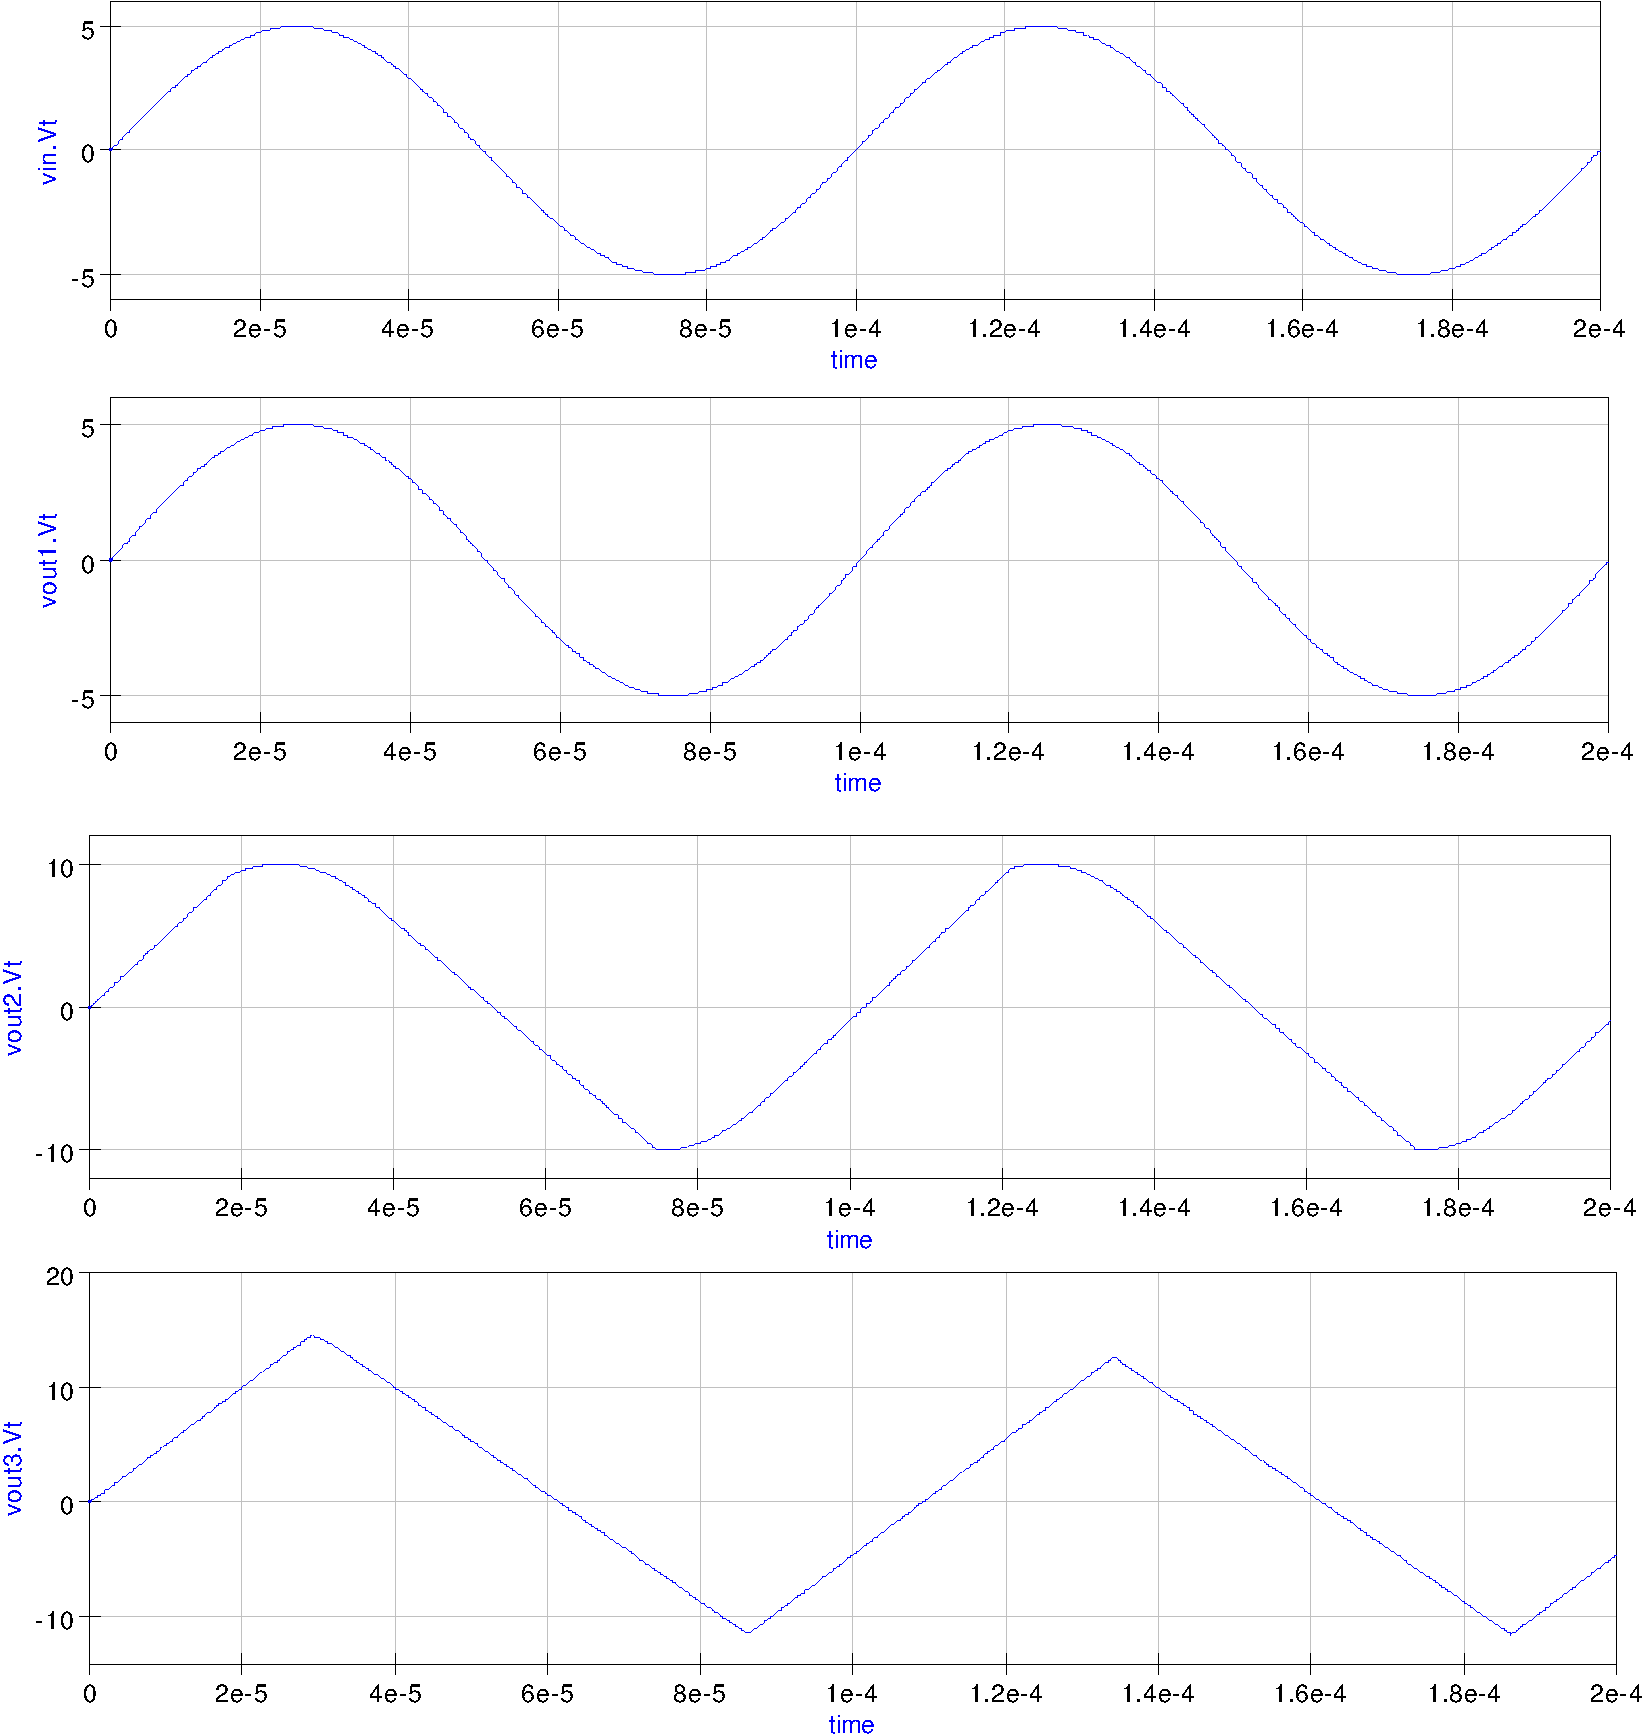
\includegraphics[width=0.9\linewidth]{fig24_dpl}
% tcomb1.png: 99.9998dpi, width=11.35cm, height=3.35cm, bb=0 0 447 132
  \caption{OP AMP slew rate simulation waveforms for the circuit shown in Fig.~\ref{fig:opamp23}.}
  \label{fig:opamp24}
\end{figure}

\tutsubsection{Modelling OP AMP overdrive and output voltage limiting}

Large transient signals can overdrive an OP AMP causing it's output voltage to saturate. On removal of the overdrive signal an OP AMP takes a finite time to recover\footnote{Overload recovery time of an OP AMP is the time required for the output voltage to recover to a rated output voltage from a saturated condition. Typical values are in the $\mu$ S region.} and return to normal linear circuit behaviour.  When saturated the output voltage is clamped at a voltage close to the plus or minus power rail voltage.  The overdrive and voltage clamping properties of an OP AMP are related and macromodels for both effects need to be added to an OP AMP model when simulating OP AMP overdrive characteristics.  However, in many circuit simulations the overdrive macromodel can be left out without loss of functionality or accuracy.\\

The effect of overdrive signals can be modelled by a voltage clamping circuit which takes account of OP AMP recovery time from voltage overdrive. This extra element clamps the output of the POLE1 module at a level above the OP AMP DC supply voltages. The overall effect of the overdrive circuit is to delay the restoration of linear circuit behaviour when an overload signal is removed.  In contrast to the overdrive module the output voltage limiting module clamps the output voltage to a voltage close to the power rail voltages, clipping any output voltage excursions above the power rail voltage levels. Figure ~\ref{fig:opamp25} illustrates the macromodels for the overdrive and output voltage limiting models, where

\begin{figure}
  \centering
  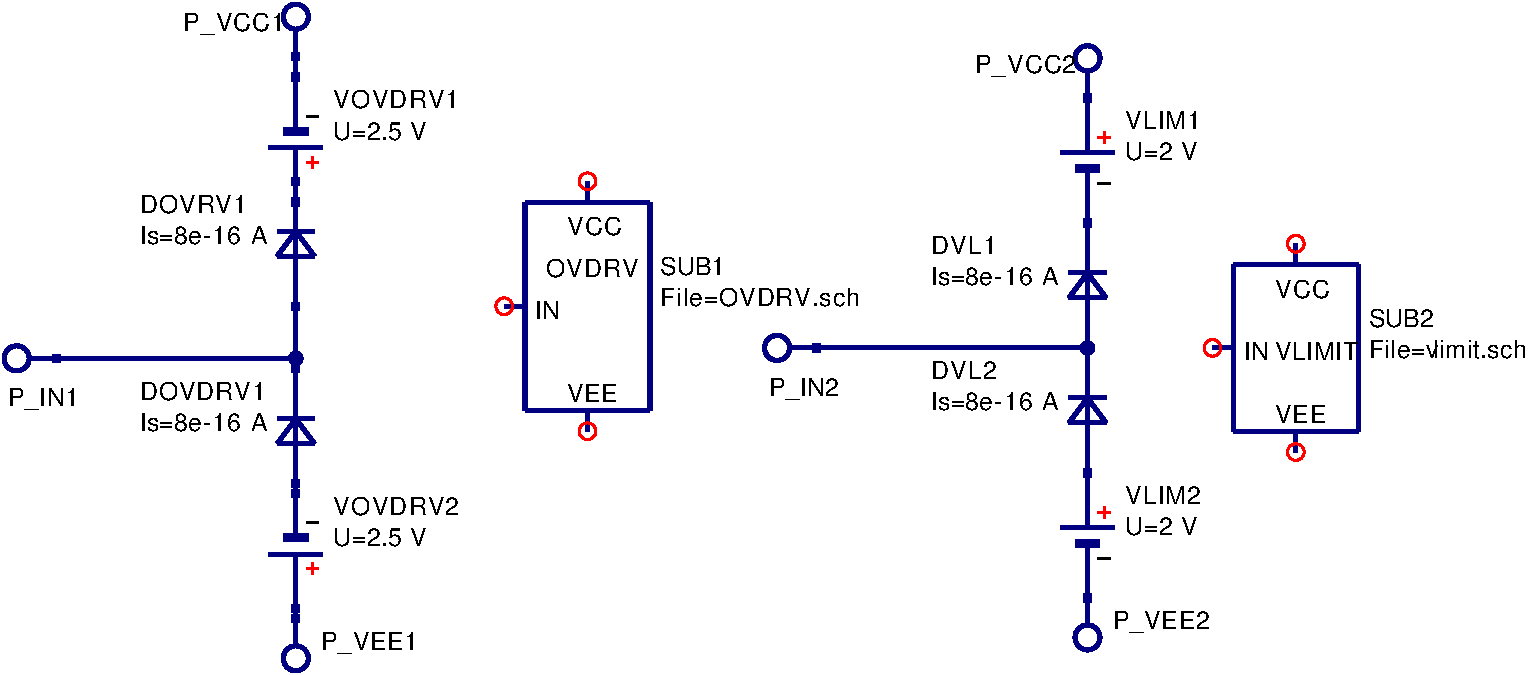
\includegraphics[width=0.9\linewidth]{fig25_sch}
% tcomb1.png: 99.9998dpi, width=11.35cm, height=3.35cm, bb=0 0 447 132
  \caption{OP AMP overdrive and output voltage limiting macromodels.}
  \label{fig:opamp25}
\end{figure}

\begin{enumerate}
\item \textit{VOVDR1} = 2.5 V = (Positive slew rate)*(Amplifier recovery time).
\item \textit{VOVDR2} = 2.5 V = (Negative slew rate)*(Amplifier recovery time).
\item \textit{VLIM1}  = 2.0 V = (+ supply voltage) - (Maximum positive output voltage) + 1 V.
\item \textit{VLIM2}  = 2.0 V = (- supply voltage) - (Maximum negative output voltage) + 1 V.
\item The diode parameters are Is = 8e-16 A, others default.
\end{enumerate}

Typical values for the UA741 OP AMP are:
\begin{enumerate}
\item Amplifier recovery time 5 $\mu$S.
\item + supply voltage =  15 V.
\item - supply voltage = -15 V.
\item Maximum positive output voltage =  14 V.
\item Maximum negative output voltage = -14 V.
\end{enumerate}

The test circuit given in Fig.~\ref{fig:opamp26} illustrates the effects of signal overdrive and output voltage clamping on a unity gain buffer circuit. The test input signal is a 1 kHz signal with the following drive voltages (1) vin1 = 10 V peak, (2) vin2 = 18 V peak, and (3) vin3 = 22 V peak. The corresponding output waveforms are shown in Fig.~\ref{fig:opamp27}. These indicate that increasing overdrive signals results in longer OP AMP recovery times before the amplifier returns to linear behaviour.
\begin{figure}
  \centering
  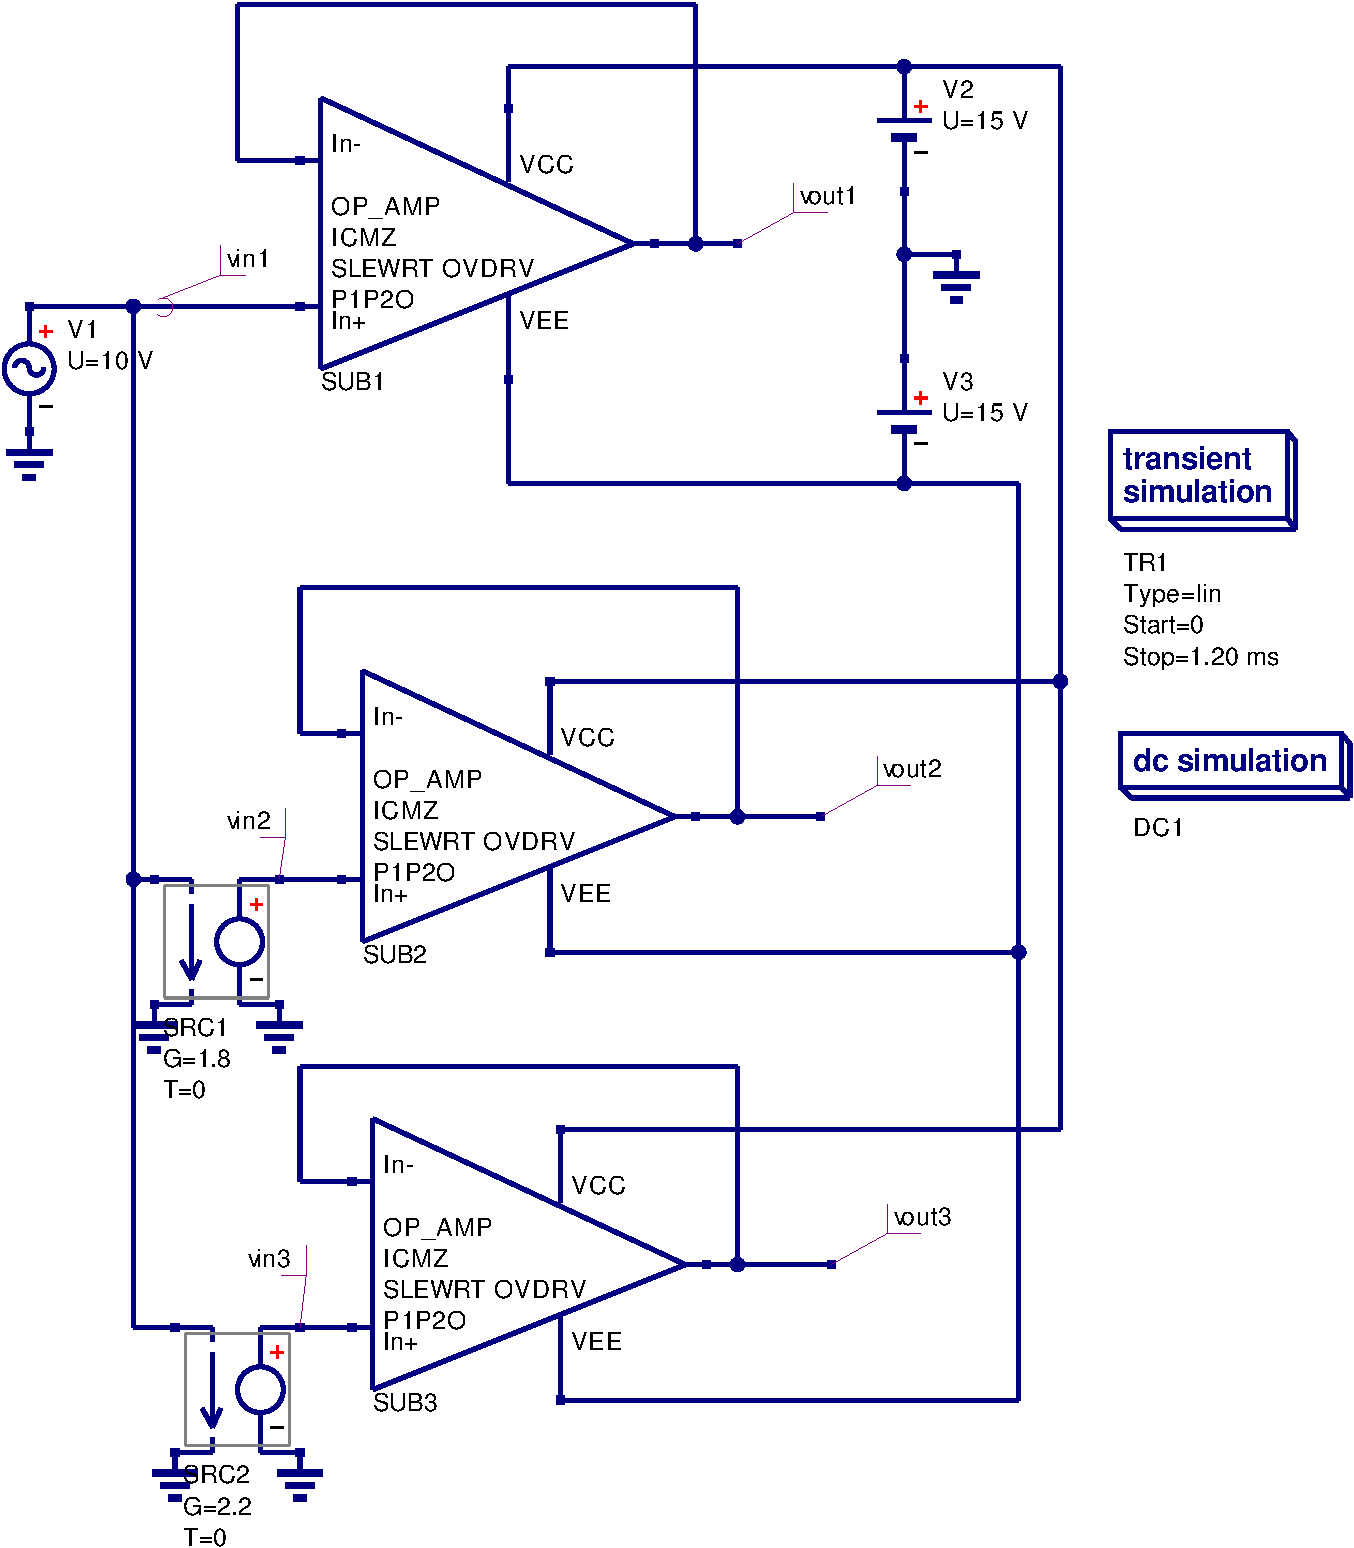
\includegraphics[width=0.9\linewidth]{fig26_sch}
% tcomb1.png: 99.9998dpi, width=11.35cm, height=3.35cm, bb=0 0 447 132
  \caption{OP AMP overdrive and output voltage limiting test circuit.}
  \label{fig:opamp26}
\end{figure}

\begin{figure}
  \centering
  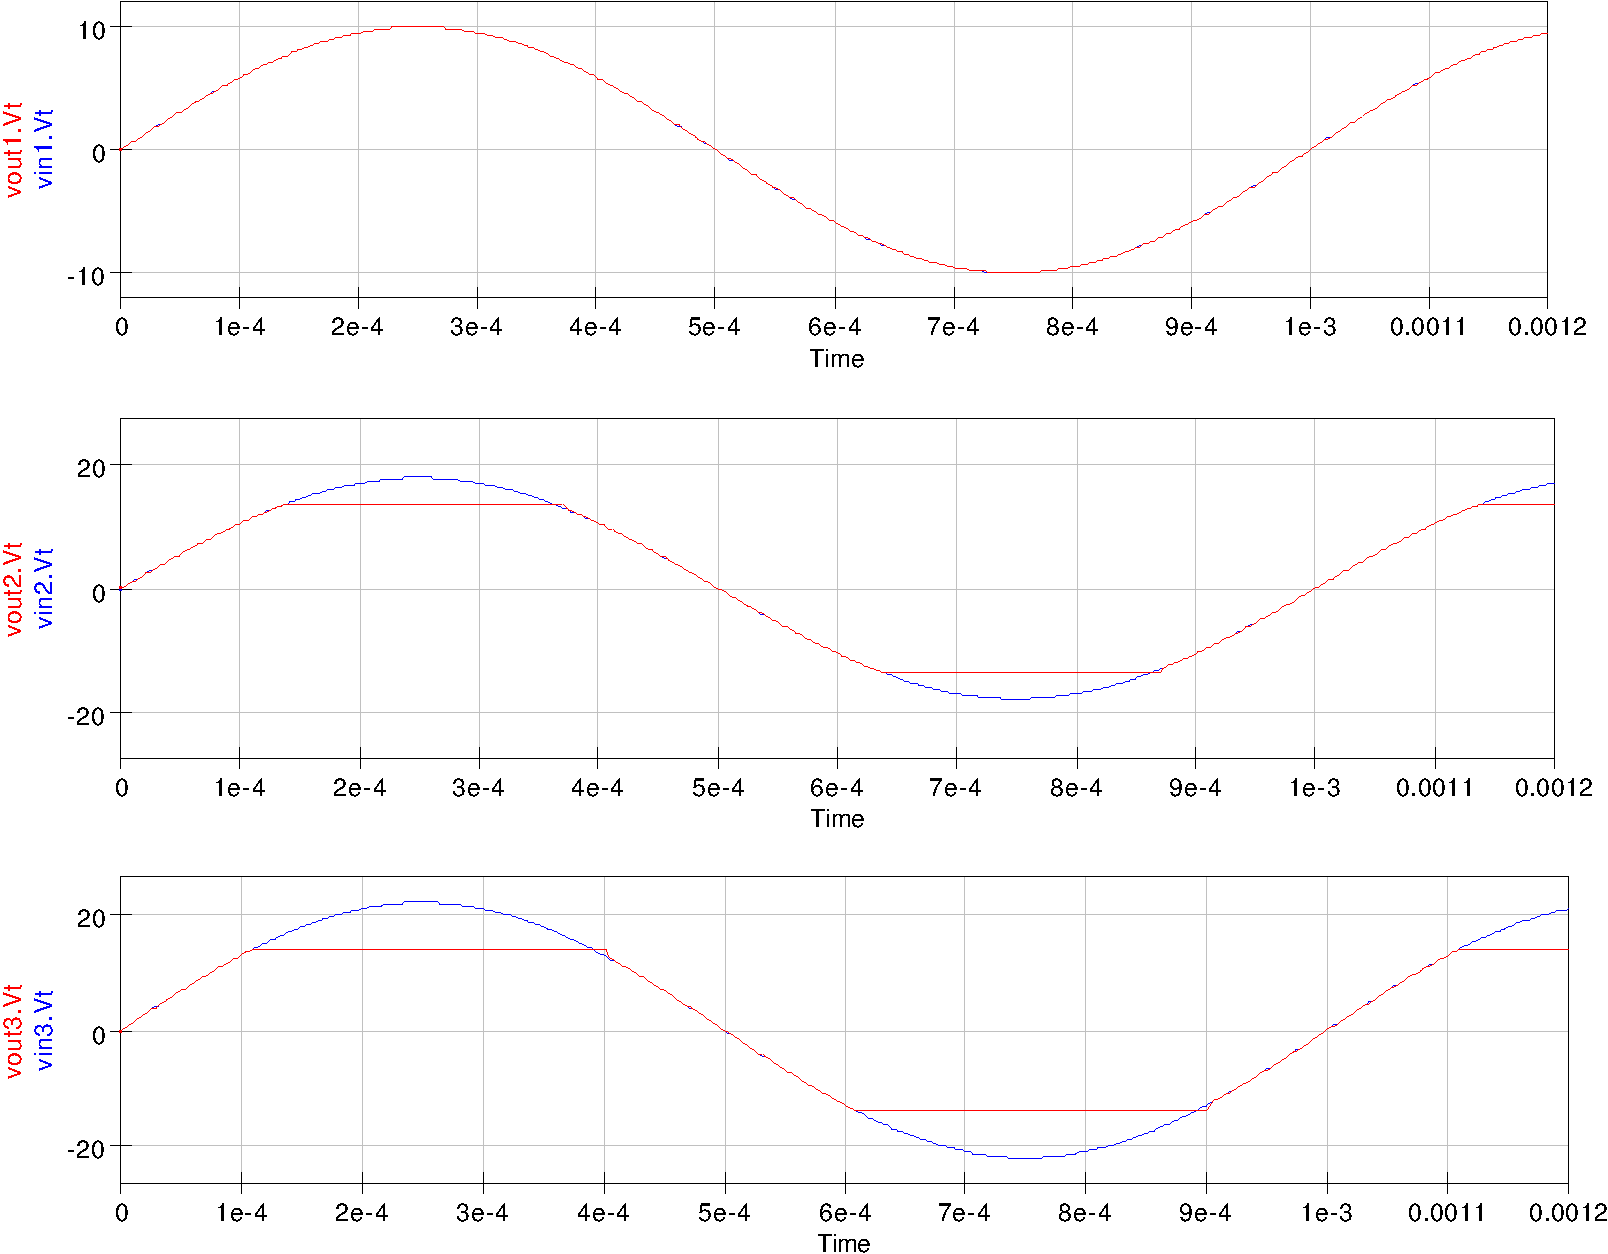
\includegraphics[width=0.9\linewidth]{fig27_dpl}
% tcomb1.png: 99.9998dpi, width=11.35cm, height=3.35cm, bb=0 0 447 132
  \caption{OP AMP overdrive and output voltage limiting waveforms for the circuit shown in Fig.~\ref{fig:opamp26}.}
  \label{fig:opamp27}
\end{figure}

\tutsubsection{Modelling OP AMP output current limiting}

Most general purpose OP AMPs have a network at the circuit output to protect the device from high load currents generated by shorting the output terminal to ground or some other situation where a high current flows through the OP AMP output stage. The electrical network shown in Fig.~\ref{fig:opamp28} acts as a current limiter: current flowing between pins \verb|P_IN1| and\verb| P_OUT1| is sensed by current controlled voltage generator HCL1. The voltage output from generator HCL1 is in series with voltage controlled generator ECL1. The connection of these generators is in opposite polarity. Hence, when the load current reaches the maximum allowed by the OP AMP either diode DCL1 or DCL2 turns on clamping the OP AMP output voltage preventing the output current from increasing.  The parameters for the current limiter macromodel are given by

\begin{enumerate}
\item \textit{RDCL1} = 100 M$\Omega$ = Dummy resistor.
\item \textit{ECL1}   G = 1.
\item \textit{HCL1}   G = 36$\Omega$ = 0.9 V/(Maximum output current A).
\item The diode parameters are Is = 1e-15 A, others default.
\end{enumerate}
 
A typical value for the UA741 OP AMP short circuit current is 34 mA at $25^{o}$C.\\



\begin{figure}
  \centering
  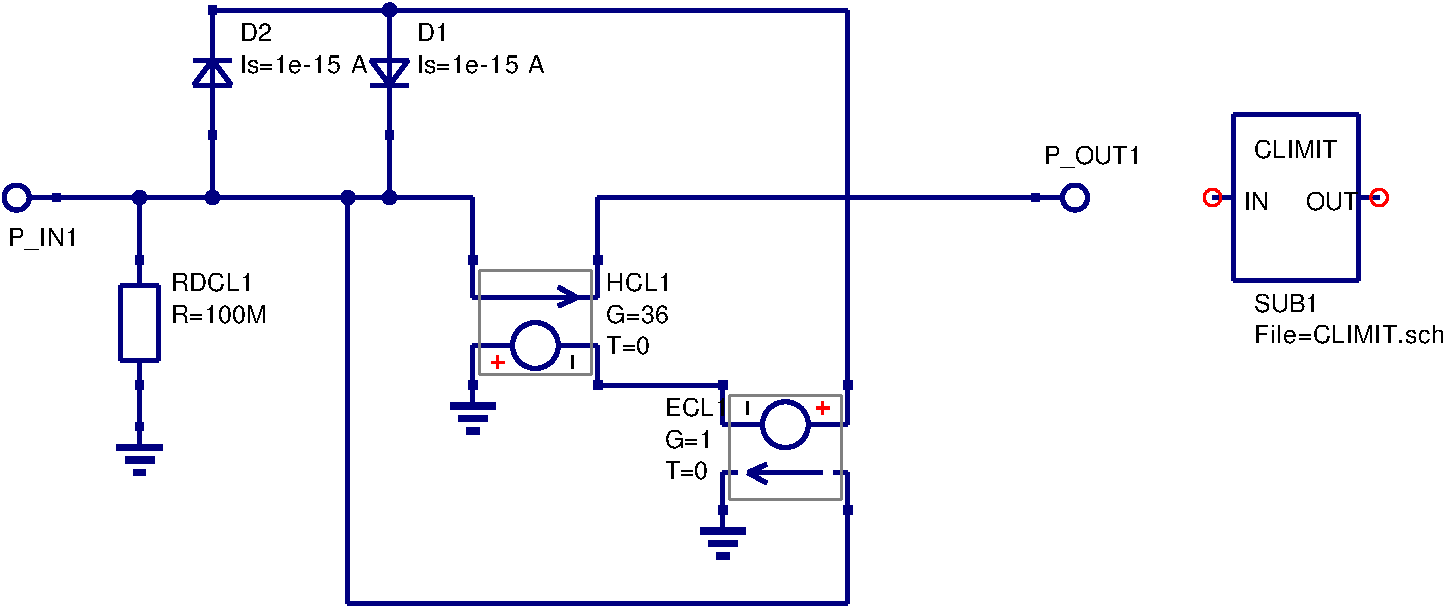
\includegraphics[width=0.9\linewidth]{fig28_sch}
% tcomb1.png: 99.9998dpi, width=11.35cm, height=3.35cm, bb=0 0 447 132
  \caption{OP AMP output current limiter macromodel.} 
  \label{fig:opamp28}
\end{figure}
 Figures~\ref{fig:opamp29} and~\ref{fig:opamp30} show a simple current limiter test circuit and the resulting test waveforms.  
 In this test circuit time controlled switches decrease the load resistors at 1 mS intervals. When the load current reaches
 roughly 34 mA the output voltage is clamped preventing further increases in load current.

\begin{figure}
  \centering
  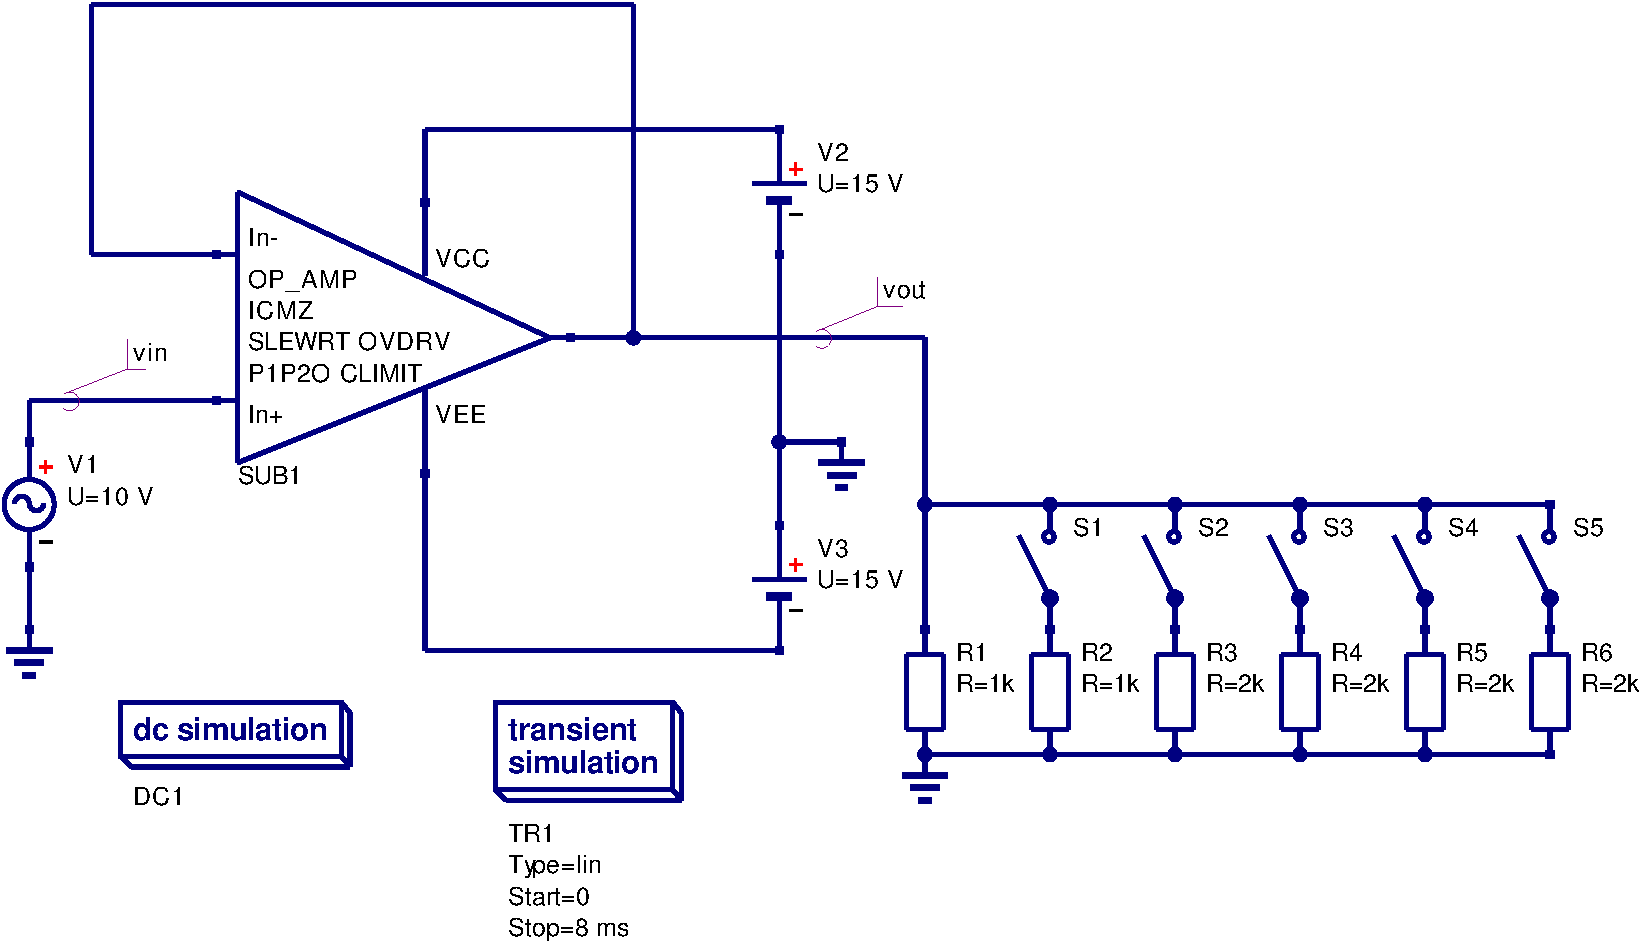
\includegraphics[width=0.9\linewidth]{fig29_sch}
% tcomb1.png: 99.9998dpi, width=11.35cm, height=3.35cm, bb=0 0 447 132
  \caption{OP AMP output current limiter test circuit.} 
  \label{fig:opamp29}
\end{figure}

\begin{figure}
  \centering
  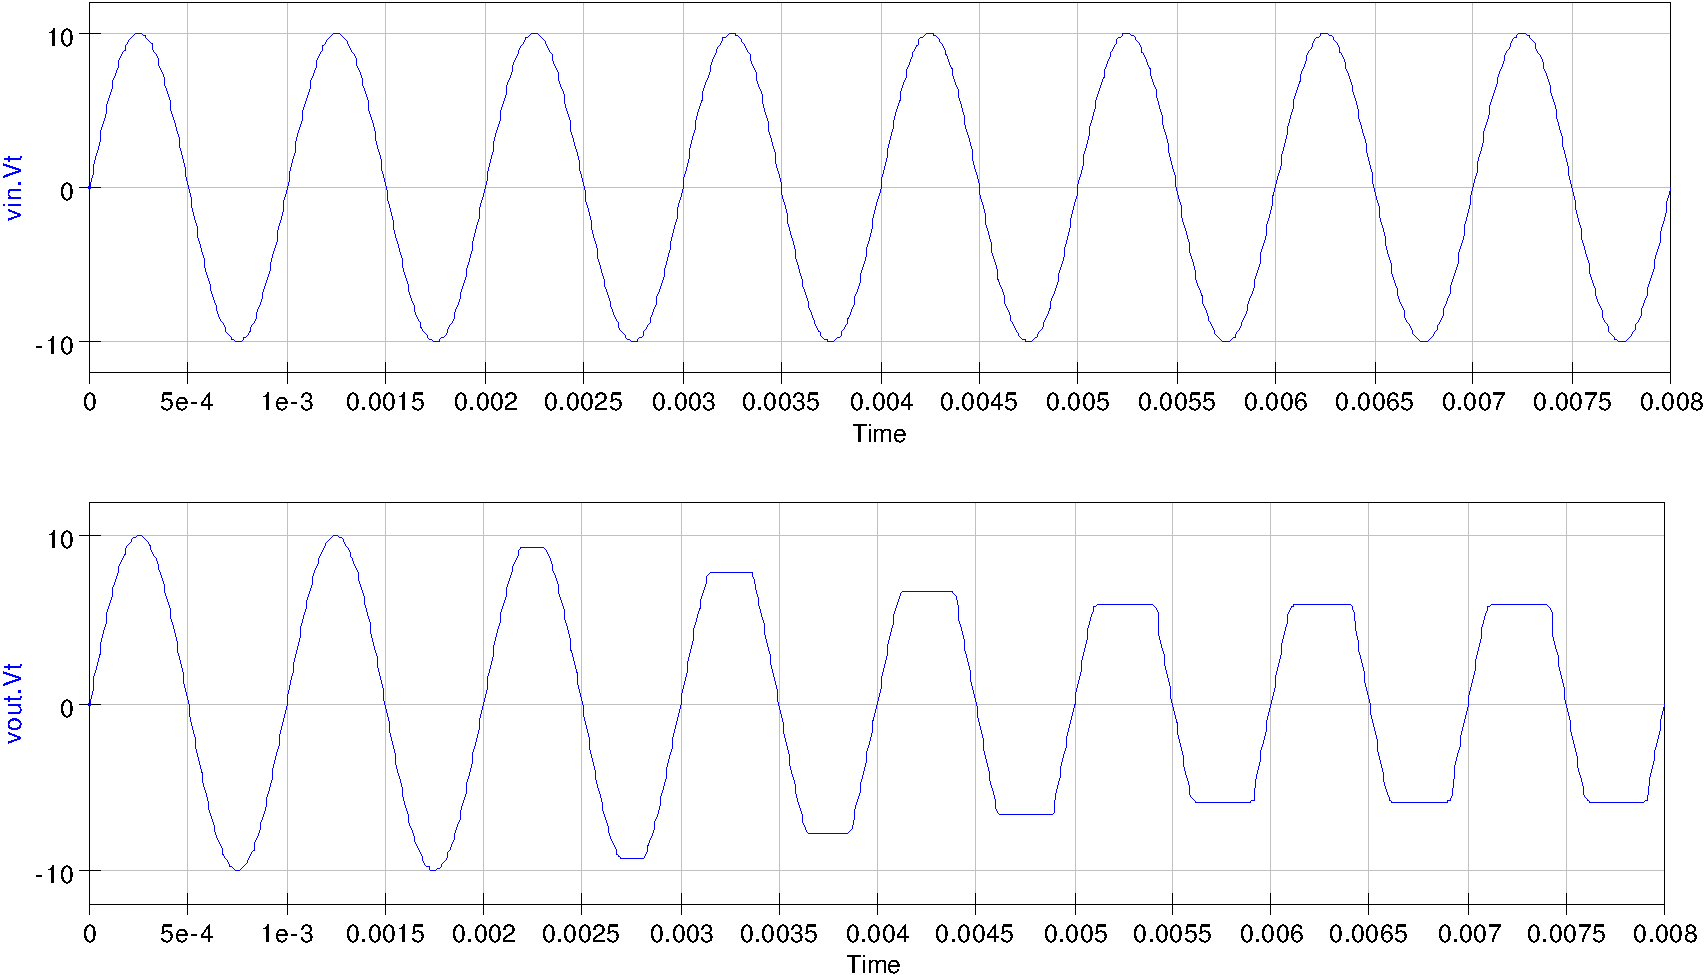
\includegraphics[width=0.9\linewidth]{fig29_dpl}
% tcomb1.png: 99.9998dpi, width=11.35cm, height=3.35cm, bb=0 0 447 132
  \caption{Simulation waveforms for current limiter test circuit shown in Fig.~\ref{fig:opamp29}.} 
  \label{fig:opamp30}
\end{figure}


\begin{table}
\centering
\begin{tabular}{lllllllllll}
Parameter & UA741 & OP27 & OP42 & OPA134 & AD746 & AD826 &  \\ 
Offset voltage (V) & 7e-4 & 30e-6 & 4e-4 & 5e-4 & 3e-4 & 5e-4 &  \\ 
Bias current (A) & 80e-9 & 15e-9 & 130e-12 & 5e-12 & 110e-12 & 3-3e-6 & \\ 
Offset current (A) & 20e-9 & 12e-9 & 6e-12 & 2e-12 & 45e-12 & 25e-9 &  \\ 
Differential input res. (ohm) & 2e6 & 4e6 & 1e12 & 1e13 & 2e11 & 300e3 &  \\ 
Differential input cap. (F) & 1.4e-12 &  & 6e-12 & 2e-12 & 5.5e-12 & 1.5e-12 & \\ 
Avd(0) dB & 106 & 125 & 120 & 120 & 109 & 75 &  \\ 
fp1 (Hz) & 5 & 6 & 20 & 5 & 0.25 & 10e3 &  \\ 
fp2 (Hz) & 3e6 & 17e6 & 20e6 & 10e6 & 35e6 & 100e6 & \\ 
CMRR(0) dB & 90 & 125 & 96 & 100 & 85 & 100 &  \\ 
fcm (Hz) & 200 & 2e3 & 100e3 & 500 & 3e3 & 2e3 &  \\ 
GBP (Hz) & 1e6 & 8e6 & 10e6 & 8e6 & 13e6 & 35e6 & \\ 
Rout (ohm) & 75 & 70 & 50 & 10 & 10 & 8 &  \\ 
Slew rate (V per micro sec.) & 0.5 & 2.8 & 50 & 20 & 75 & 300 &  \\ 
Overdrive recovery time (S) & 5e-6 &   & 700e-9 & 0.5e-6 &   &   & \\ 
DC supply current (A) & 1.4e-3 & 2.5e-3 & 5.1e-3 & 4e-3 & 7e-3 & 6.6e-3 & \\ 
Short circuit output current(A) & 34e-3 & 32e-3 & 30e-3 & 40e-3 & 25e-3 & 90e-3 &  \\ 
Common-mode input res. (ohm) & 1.3e8  & 2e9 &   & 1e13 & 2.5e11 &   &  \\ 
Common-mode input cap. (F) &   &   &   & 5e-12 & 5.5e-12 &   & 
\end{tabular}
\caption{Typical OP AMP parameters taken from device data sheets.}
\label{tab:tab1}
\end{table}

\tutsection{Obtaining OP AMP macromodel parameters from published device data}
The OP AMP modular macromodel has one very distinct advantage when compared to other amplifier models namely that it is possible to derive the macromodel parameters directly from a common set characteristics found on the majority of manufacturer's data sheets. The data given in Table.~\ref{tab:tab1} shows a typical range of values found on OP AMP data sheets.  In cases where a particular parameter is not given then a starting point is to use a value obtained from a data sheet of an equivalent device. The macromodel element values are then calculated using the equations presented in the previous sections of this tutorial.  As a rule of thumb it is good practice to test each block in the modular macromodel prior to constructing a complete OP AMP macromodel.


\tutsection{More complete design examples.}

In this section two larger design examples are presented. These demonstrate the characteristics of the various OP AMP macromodels introduced in the previous text and attempt to give readers guidance as to the correct model to choose for a particular simulation.

\tutsubsection{Example 1: State variable filter design and simulation} 

The circuit given in Fig.~\ref{fig:opamp31} is a state variable filter which simultaneously generates band-pass, high-pass and low-pass responses. The circuit consists of an OP AMP adder and two integrator circuits and requires three OP AMPS, two capacitors and a number of resistors.  The selection of the type of OP AMP for successful operation of this filter is critical because devices with high offset voltage will cause the integrators to saturate and the circuit will not function correctly. For operation below 20 kHz the OP27 is a good choice of OP AMP because of it's low offset voltage in the $\mu$V region. In this simulation both the DC characteristics and small signal AC transfer characteristics are needed to check the filter design, hence the AC macromodel with the DC parameters embedded in the input stage should allow accurate modelling of the filter performance.\footnote{The magnitude of the output signals from the filter should also be checked to ensure that these signals do not exceed the power supply voltages.}  The insert in Fig.~\ref{fig:opamp31} list the DC output voltages for each of the OP AMP stages indicating that the integrators are not saturated.  The design of the state variable filter uses the following equations:
\begin{enumerate}
\item The superposition principle yields
\begin{equation}
vhp = -\dfrac{R1}{R6}vin-\dfrac{R1}{R7}vlp+\left( 1+\dfrac{R1}{R7 \parallel R6} \right) \dfrac{R4}{R4+R5}vbp
\end{equation}
When $R1= R6 =R7$

\begin{equation}
vhp = -vin -vlp +  \dfrac{3R4}{R4+R5}vbp
\end{equation}

\item Also
\begin{equation}
vbp = -\dfrac{1}{j\frac{f}{f_{0}}}vhp
\end{equation}
where 
\begin{equation}
f_{0}=\dfrac{1}{2 \pi R_{2}C_{1}} = \dfrac{1}{2 \pi R_{3}C_{2}}
\end{equation} 

\item Similarly
\begin{equation}
vlp = -\dfrac{1}{j\frac{f}{f_{0}}}vbp = -\dfrac{1}{(\frac{f}{f_{0}})^{2}}vhp  
\end{equation}

\item Hence
\begin{equation}
\dfrac{vhp}{vin}=\dfrac{(\frac{f}{f_{0}})^{2}}{1-(\frac{f}{f_{0}})^{2}+(\frac{j}{Q})(\frac{f}{f_{0}})}
\end{equation}
Where
\begin{equation}
Q = \dfrac{1}{3}(1+\dfrac{R5}{R4})
\end{equation}

\item Also
\begin{equation}
\dfrac{vbp}{vin}=\dfrac{j\frac{f}{f_{0}}}{1-(\frac{f}{f_{0}})^{2}+(\frac{j}{Q})(\frac{f}{f_{0}})}
\end{equation}

\item Also
\begin{equation}
\dfrac{vlp}{vin}=\dfrac{-1}{1-(\frac{f}{f_{0}})^{2}+(\frac{j}{Q})(\frac{f}{f_{0}})}
\end{equation}

\end{enumerate}

Assuming $f_{0}$ = 1 kHz and the required bandwidth of the band pass filter is 10 Hz, on setting $R1 = R6 = R7 = 47 k\Omega$ and $C1 = C2 = 2.2 nF$, calculation yields $R2 = R3 = 72.33 k\Omega$\footnote{The values of $R2$ and $R3$ need to be trimmed if the filter center frequency and bandwidth are required to high accuracy.}  In this design $Q = 1k/10 = 100$.  Hence setting $R4 = 1k\Omega$ yields $R5 = 294k\Omega$ (1 \verb|%| tolerance). The simulation waveforms for the band pass output are given in Fig.~\ref{fig:opamp32} \footnote{Note that the input signal $vin$ has been set at 0.1 V peak.  The circuit has a Q factor of 100 which means that the band pass output voltage is 10 V peak. Input signals of amplitude much greater than 0.1 V are likely to drive the output signal into saturation when the power supply voltages are $\pm15 V$.}.  When the circuit Q factor is reduced to lower values the other filter outputs act as traditional high and low pass filters. The simulation results for Q factor one are shown in Fig.~\ref{fig:opamp33}.
\begin{figure}
  \centering
  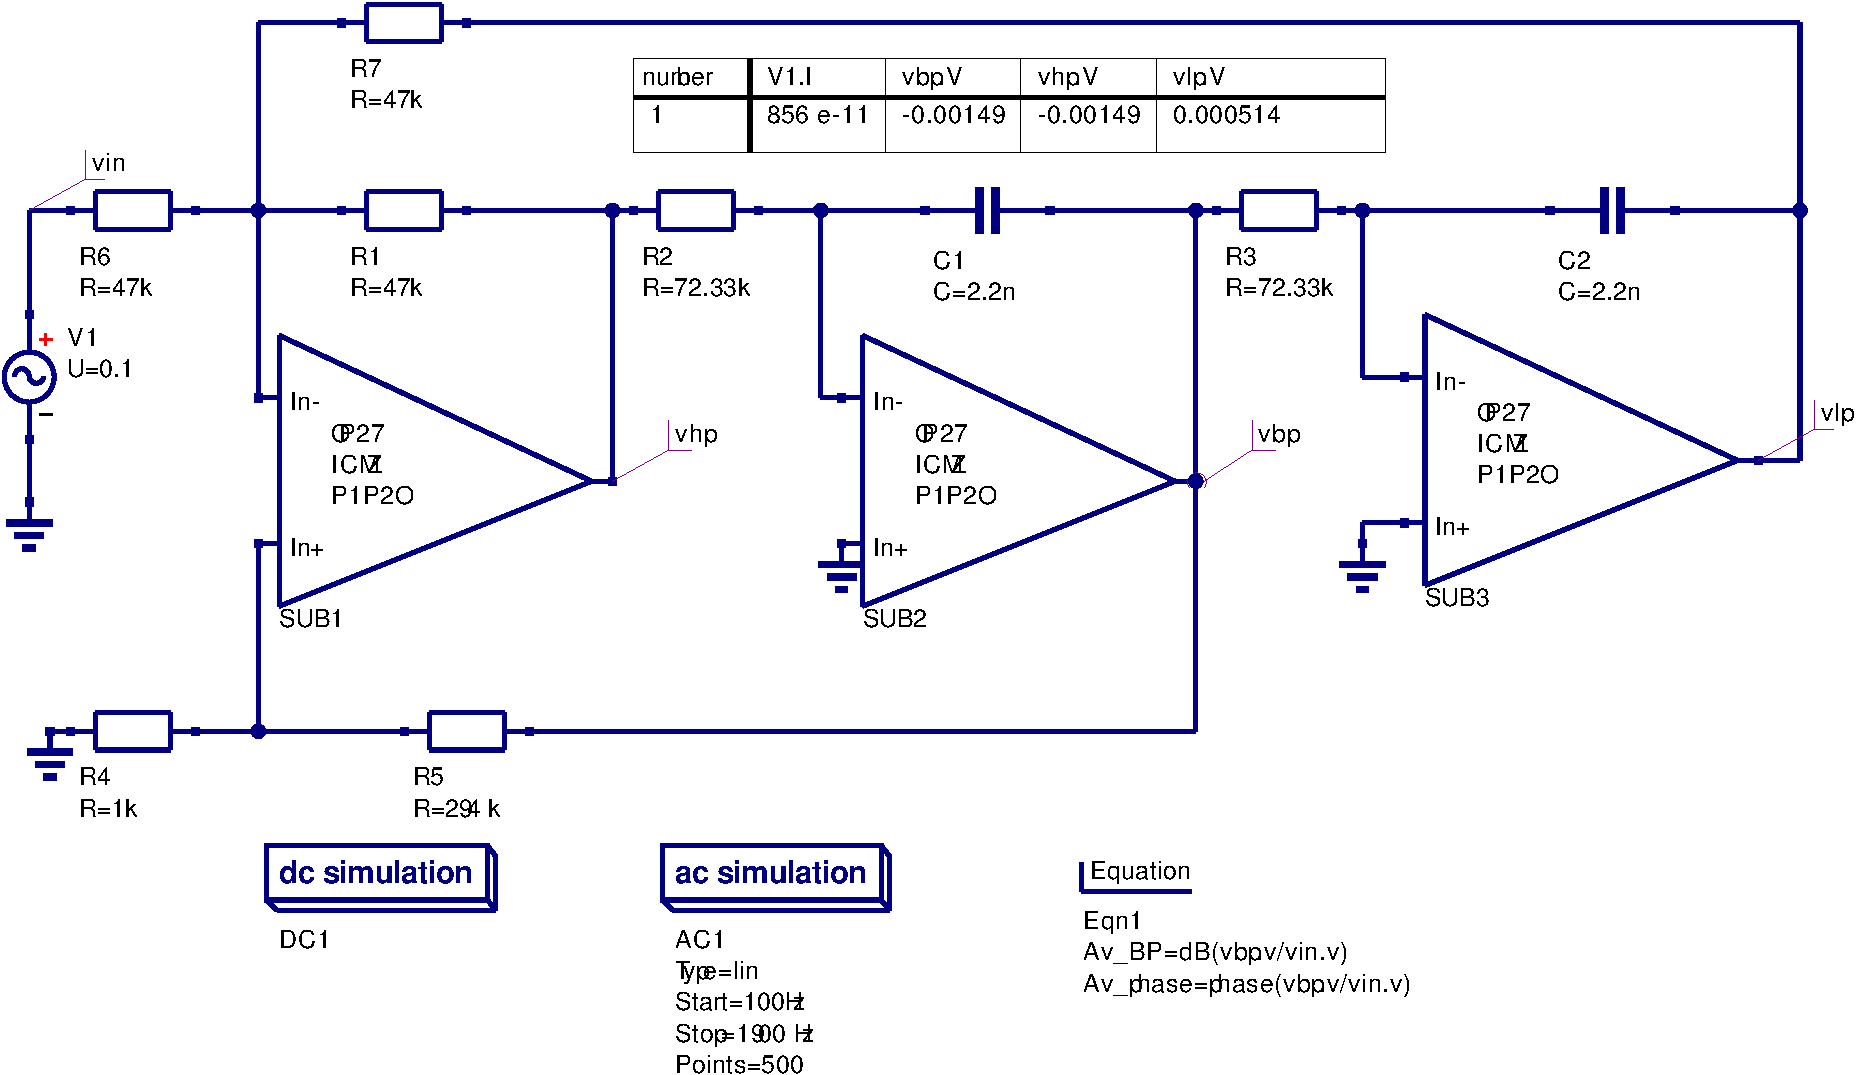
\includegraphics[width=0.9\linewidth]{fig31_sch} 
% tcomb1.png: 99.9998dpi, width=11.35cm, height=3.35cm, bb=0 0 447 132
  \caption{Three OP AMP state variable filter.} 
  \label{fig:opamp31}
\end{figure}

\begin{figure}
  \centering
  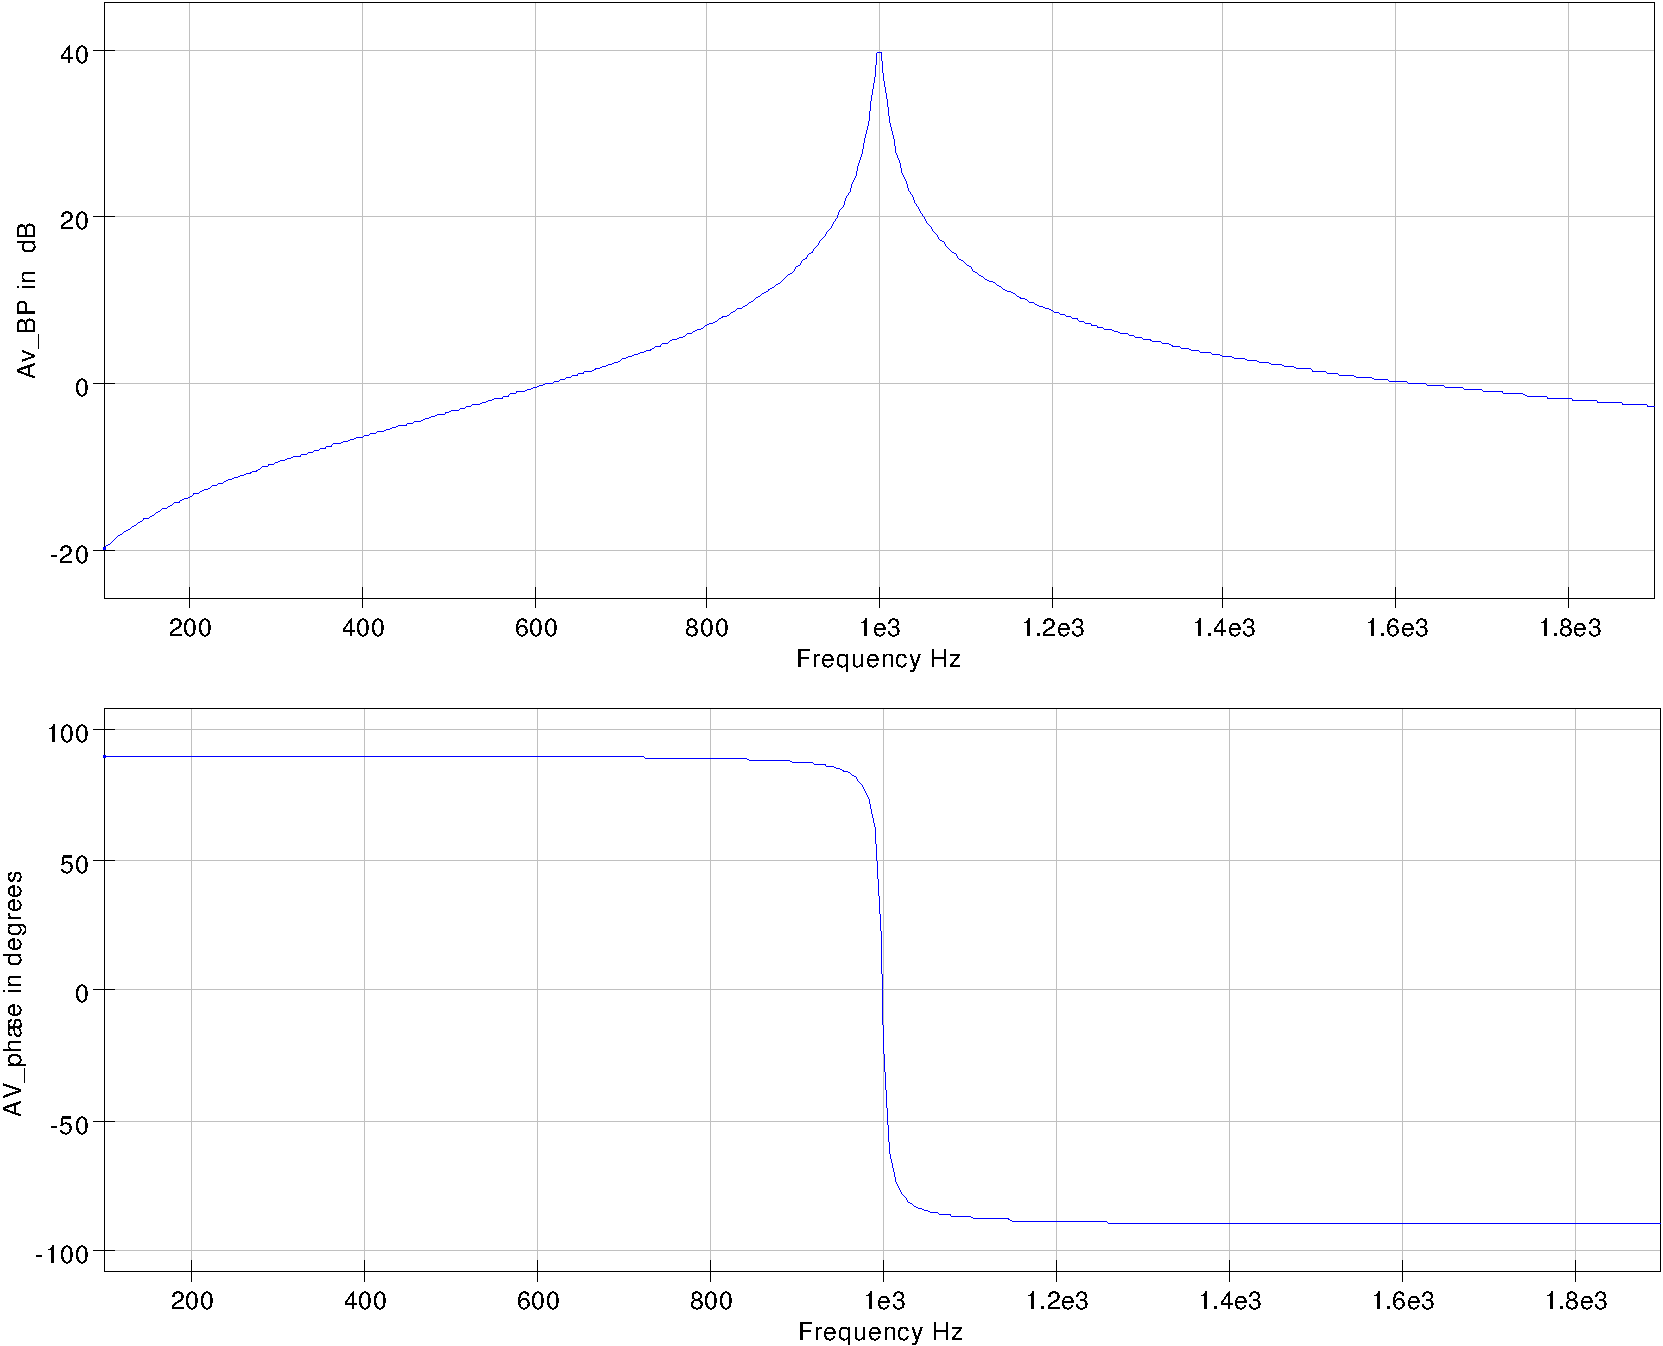
\includegraphics[width=0.9\linewidth]{fig31_dpl}
% tcomb1.png: 99.9998dpi, width=11.35cm, height=3.35cm, bb=0 0 447 132
  \caption{Simulation waveforms for current state variable filter circuit shown in Fig.~\ref{fig:opamp31}.} 
  \label{fig:opamp32}
\end{figure}

\begin{figure}
  \centering
  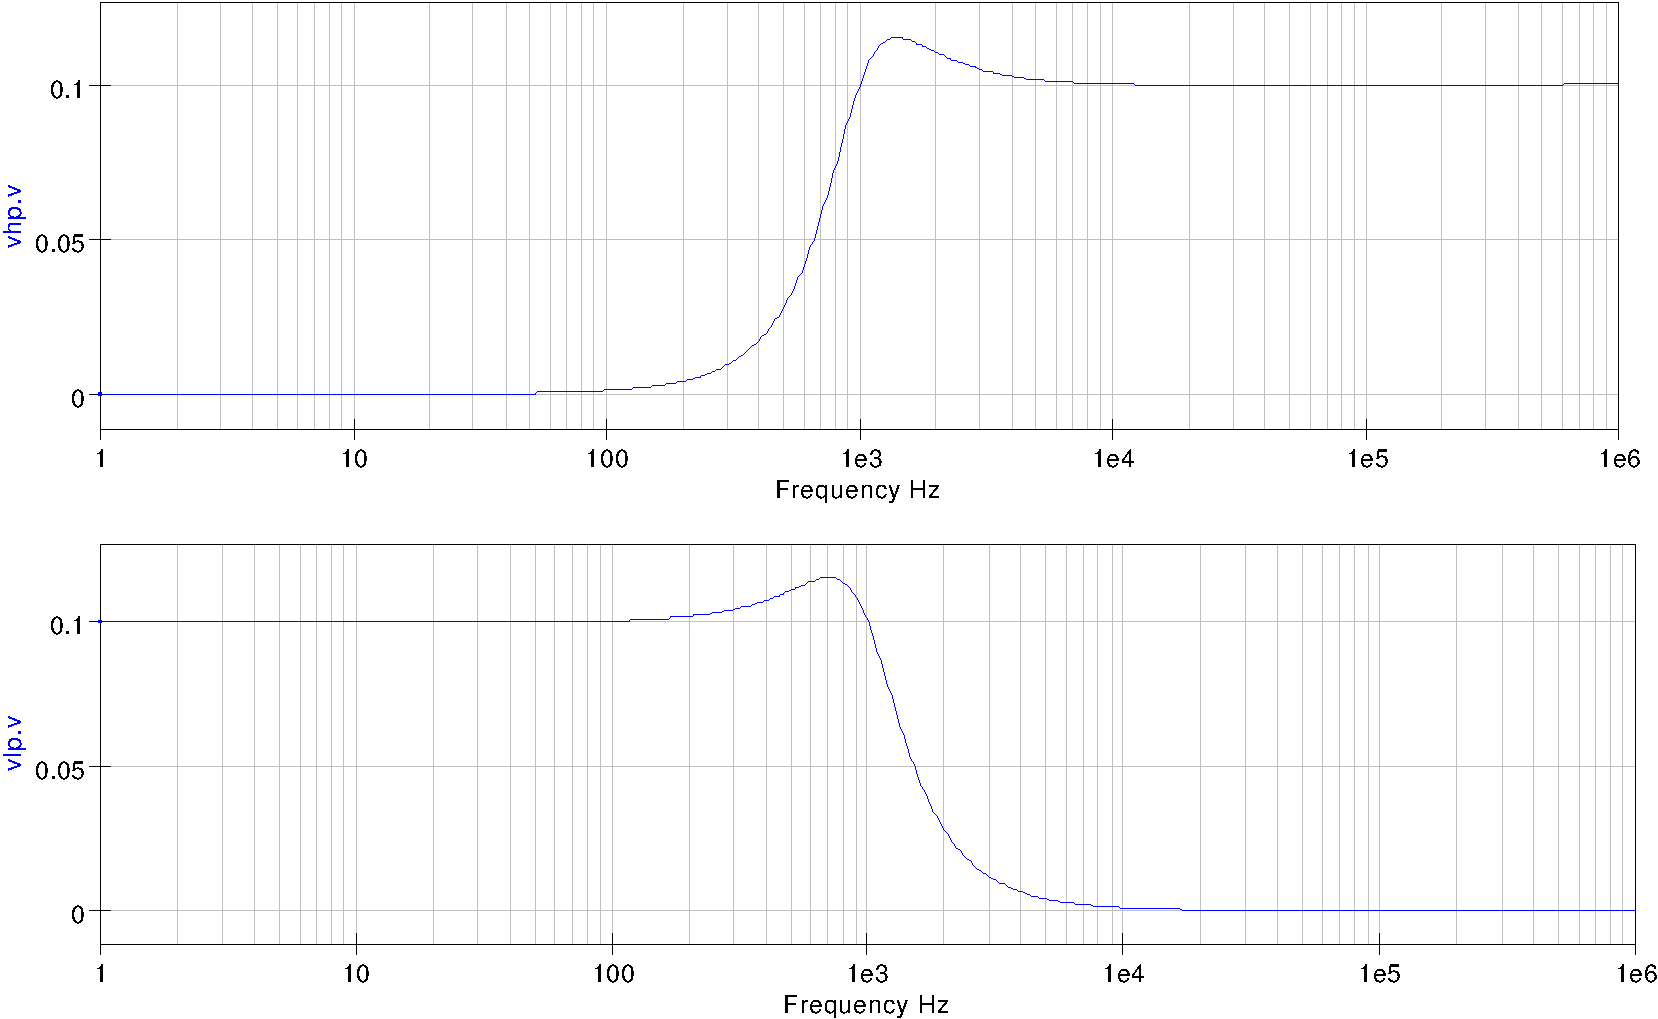
\includegraphics[width=0.9\linewidth]{fig33_dpl}
% tcomb1.png: 99.9998dpi, width=11.35cm, height=3.35cm, bb=0 0 447 132
  \caption{State variable low pass and high pass response for $Q = 1$, $R5 = 2k\Omega$.} 
  \label{fig:opamp33}
\end{figure}

\tutsubsection{Example 2: Sinusoidal signal generation with the Wien bridge oscillator} 

The Wien bridge sinusoidal oscillator has become a classic due to it's simplicity and low distortion capabilities.  It is an ideal vehicle for demonstrating the properties of OP AMP macromodels and indeed the performance of circuit simulators. Shown in Fig.~\ref{fig:opamp35} is the basic Wien bridge oscillator which consists of a single OP AMP with negative and positive feedback circuits. The design equations for this circuit are

\begin{enumerate}
\item  Non-inverting amplifier.
\begin{equation}
\dfrac{vout}{v+} = 1 + \dfrac{R3}{R4}
\end{equation}

\item Feedback factor
\begin{equation}
b = \dfrac{vout}{v+} =\dfrac{1}{3+j(\frac{f}{f_{0}}-\frac{f_{0}}{f})}
\end{equation}
Where $f_{0} = \dfrac{1}{2\pi R1 C1} =\dfrac{1}{2\pi R2 C2} $

\item Loop gain

The oscillator loop gain $b A_{v}$ must equal one for stable oscillations. Hence,
\begin{equation}
b A_{v} = \dfrac{1+\frac{R3}{R4}}{3+j(\frac{f}{f_{0}}-\frac{f_{0}}{f})}
\end{equation}

Moreover, at $f = f_{0}$,  
\begin{equation}
b A_{v} = \dfrac{1+\frac{R3}{R4}}{3}
\end{equation}

Setting $R3/R4$ slightly greater than two causes oscillations to start and increase in amplitude during each oscillatory cycle. Furthermore, if $R3/R4$ is less than two oscillations will never start or decrease to zero.
\end{enumerate}

Figure~\ref{fig:opamp36} shows a set of Wien bridge oscillator waveforms. In this example the OP AMP is modelled using the OP27 AC macromodel. This has been done deliberately to demonstrate what happens with a poor choice of OP AMP model.  The oscillator frequency is 10 kHz with both feedback capacitors and resistors having equal values. Notice that the oscillatory output voltage continues to grow with increasing time until it's value far exceeds the limit set by a practical OP AMP power supply voltages.  The lower of the two curves in Fig.~\ref{fig:opamp36} illustrates the frequency spectrum of the oscillator output signal. The data for this curve has been generated using the Time2Freq function.  Adding slew rate and voltage limiting to the OP27 macromodel will limit the oscillator output voltage excursions to the OP AMP power supply values. The waveforms for this simulation are shown in Fig.~\ref{fig:opamp37}.  When analysing transient response data using function Time2Freq it is advisable to restrict the analysis to regions of the response where the output waveform has reached a steady state otherwise the frequency spectrum will include effects due to growing, or decreasing, transients.  The voltage limiting network clips the oscillator output voltage restricting its excursions to below the OP AMP power supply voltages.  The clipping is very visible in Fig.~\ref{fig:opamp37}.  Notice also that the output waveform is distorted and is no longer a pure sinusoidal waveform of 10 kHz frequency.  Odd harmonics are clearly visible and the fundamental frequency has also decreased due to the signal saturation distortion.  In a practical Wien bridge oscillator the output waveform should be a pure sinusoid with zero or little harmonic distortion.  One way to achieve this is to change the amplitude of the OP AMP gain with changing signal level: as the output signal increases so $Av$ is decreased or as the output signal level decreases $Av$ is increased.  At all times the circuit parameters are changed to achieve the condition $b Av = 1$.  The circuit shown in Fig.~\ref{fig:opamp38} uses two diodes and a resistor to automatically change the OP AMP closed loop gain with changing signal level.  Fig.~\ref{fig:opamp39} shows the corresponding waveforms for the Wien bridge circuit with automatic gain control.  Changing the value of resistor $R5$ causes the amplitude of the oscillator output voltage to stabilise at a different value; decreasing $R5$ also decreases $vout$. The automatic gain control version of the Wien bridge oscillator also reduces the amount of harmonic distortion generated by the oscillator.  This can be clearly observed in Fig.~\ref{fig:opamp39}.  Changing the oscillator frequency can be accomplished by either changing the capacitor or resistor values in the feedback network $b$. To demonstrate how this can be done using Qucs, consider the circuit shown in Fig.~\ref{fig:opamp40}.  In this circuit time controlled switches change the value of both capacitors as the simulation progresses.  The recorded output waveform for this circuit is shown in Fig.~\ref{fig:opamp41}.


\begin{figure}
  \centering
  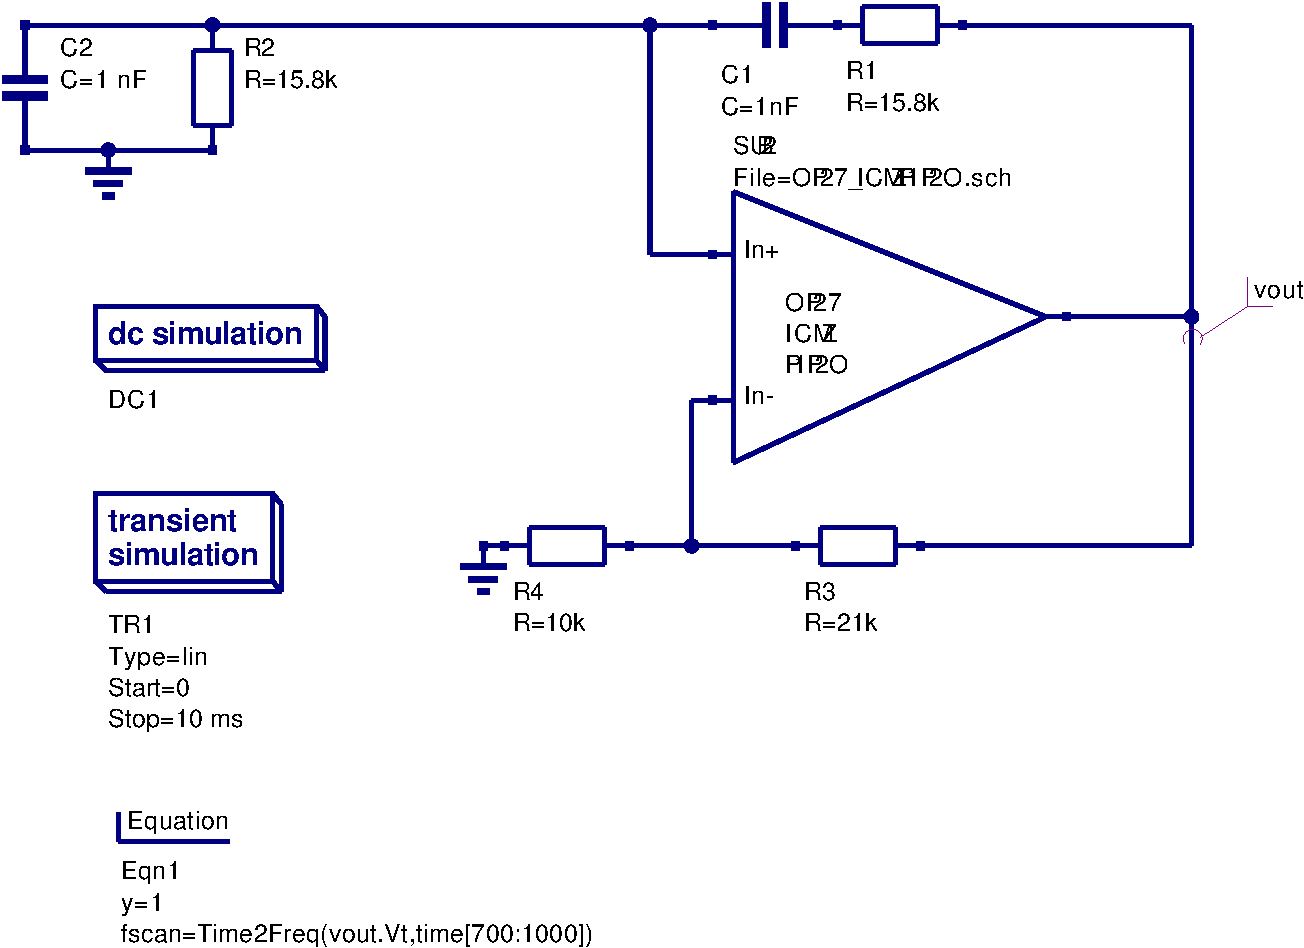
\includegraphics[width=0.9\linewidth]{fig34_sch}
% tcomb1.png: 99.9998dpi, width=11.35cm, height=3.35cm, bb=0 0 447 132
  \caption{Classic Wien bridge sinusoidal oscillator.} 
  \label{fig:opamp35}
\end{figure}

\begin{figure}
  \centering
  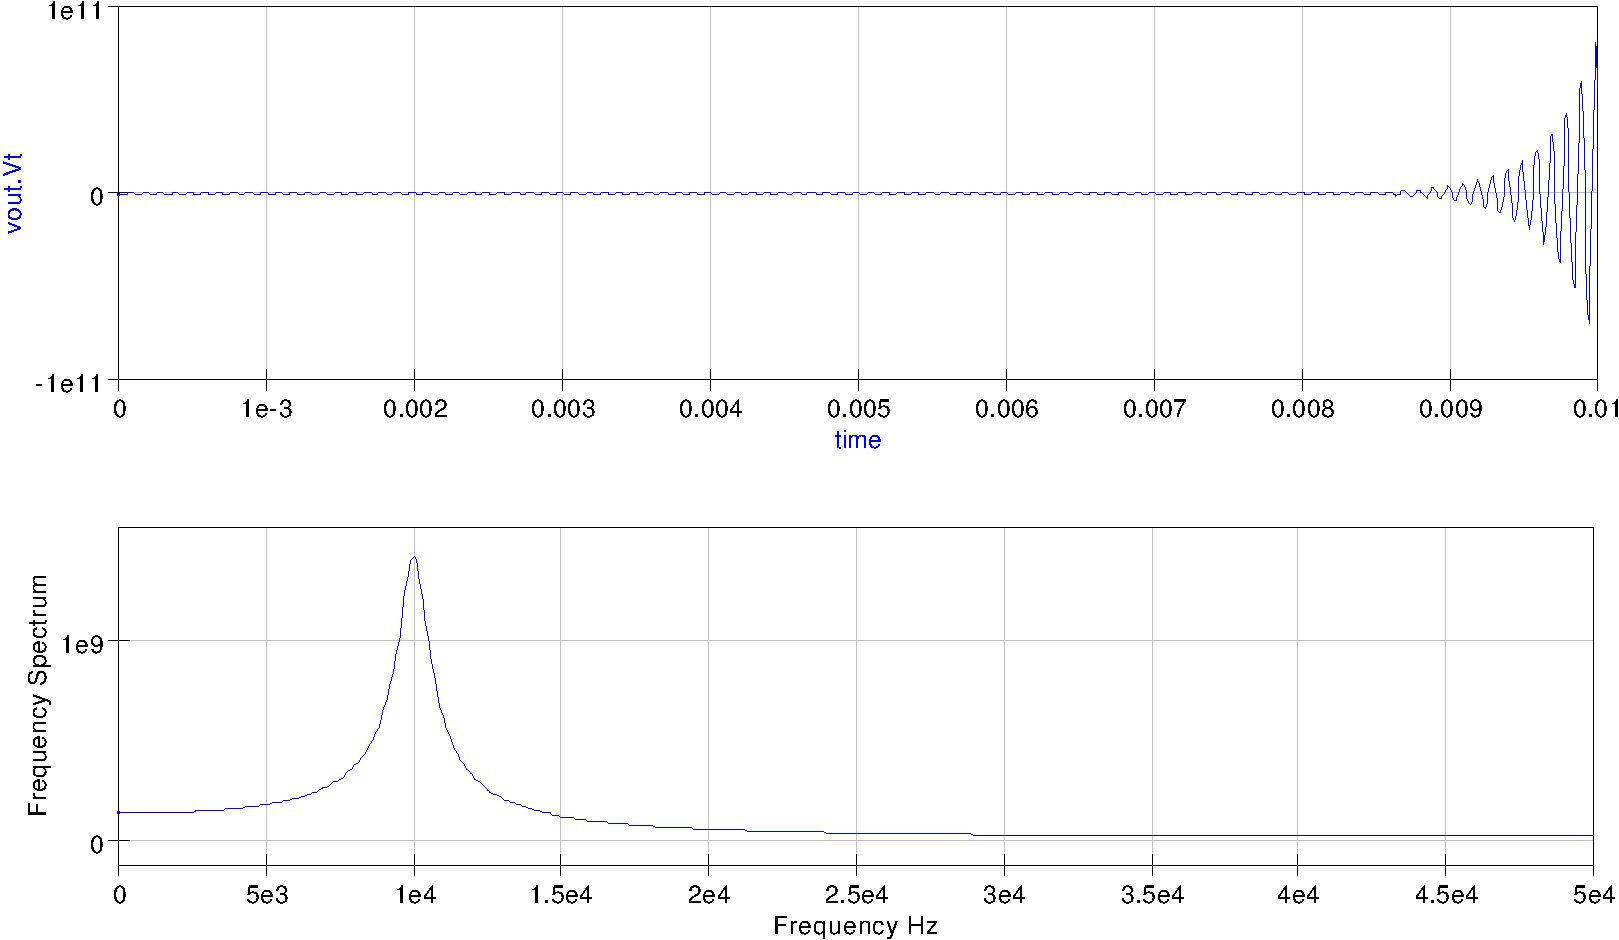
\includegraphics[width=0.9\linewidth]{fig34_dpl}
% tcomb1.png: 99.9998dpi, width=11.35cm, height=3.35cm, bb=0 0 447 132
  \caption{Simulation waveforms for the circuit shown in Fig.~\ref{fig:opamp35}: OP27 AC macromodel. } 
  \label{fig:opamp36}
\end{figure}

\begin{figure}
  \centering
  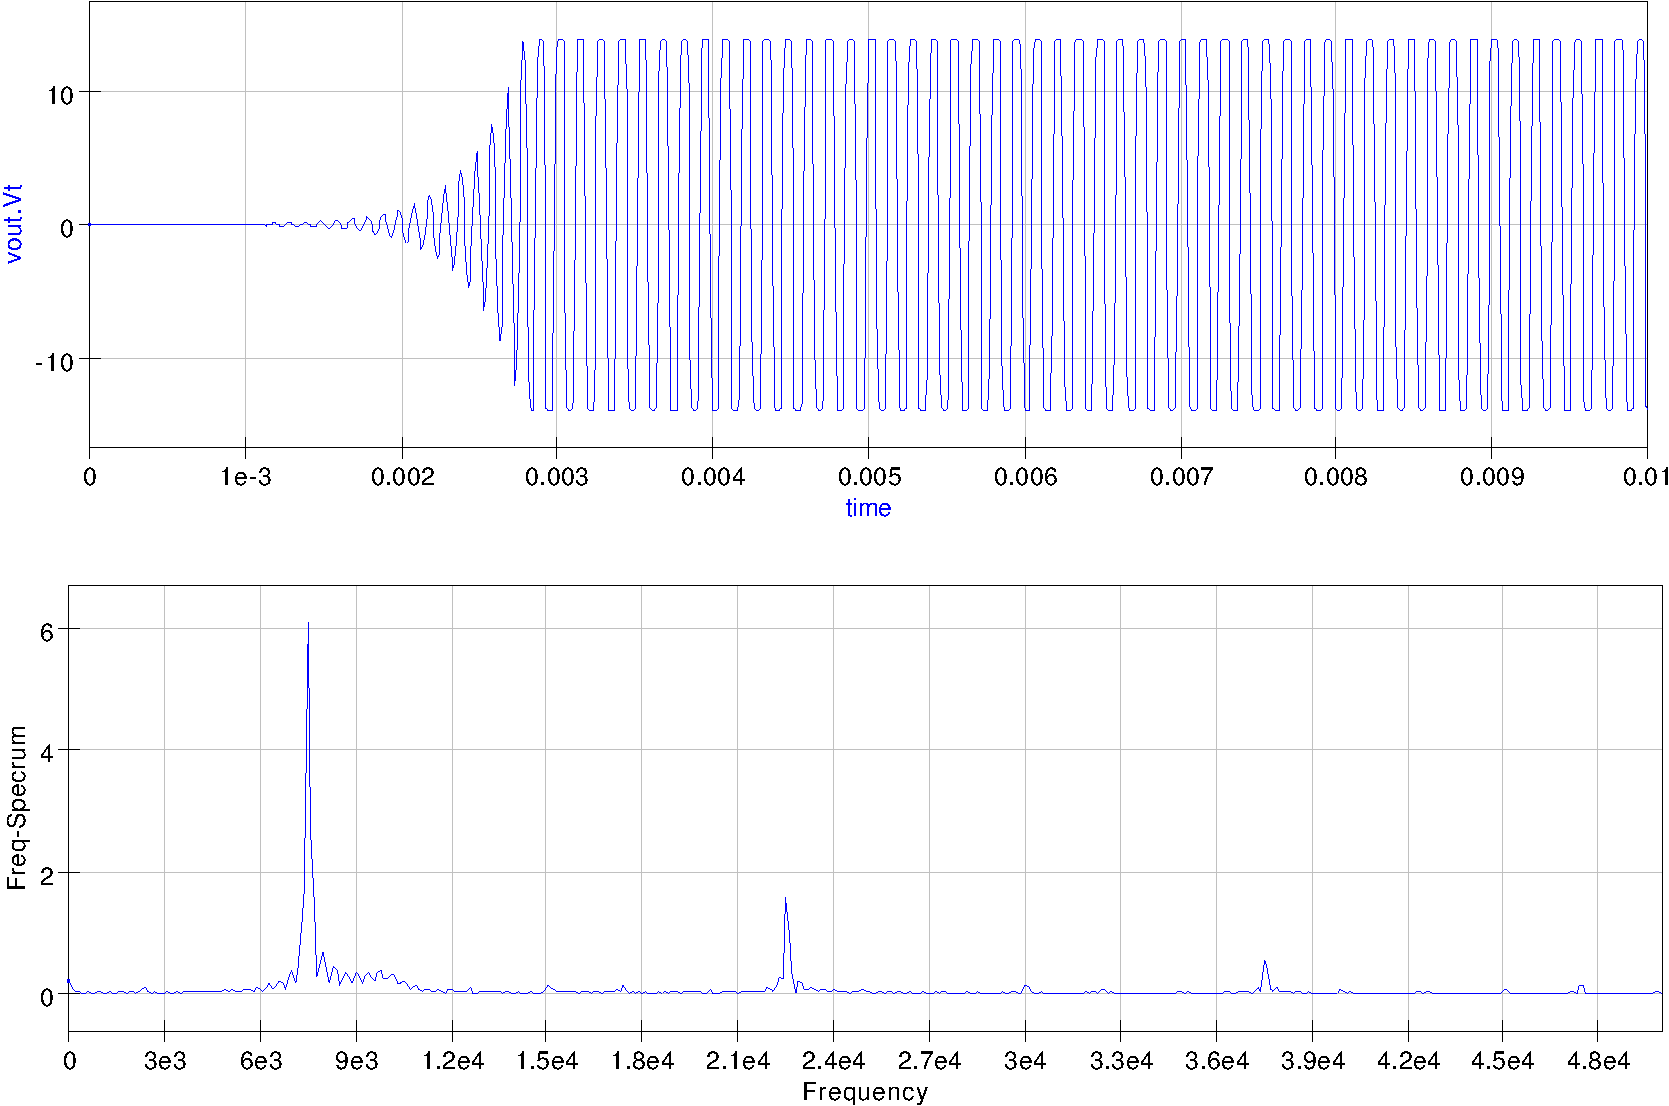
\includegraphics[width=0.9\linewidth]{fig37_dpl}
% tcomb1.png: 99.9998dpi, width=11.35cm, height=3.35cm, bb=0 0 447 132
  \caption{Simulation waveforms for the circuit shown in Fig.~\ref{fig:opamp35}: OP27 AC + slew rate + vlimit macromodel. } 
  \label{fig:opamp37}
\end{figure}

\begin{figure}
  \centering
  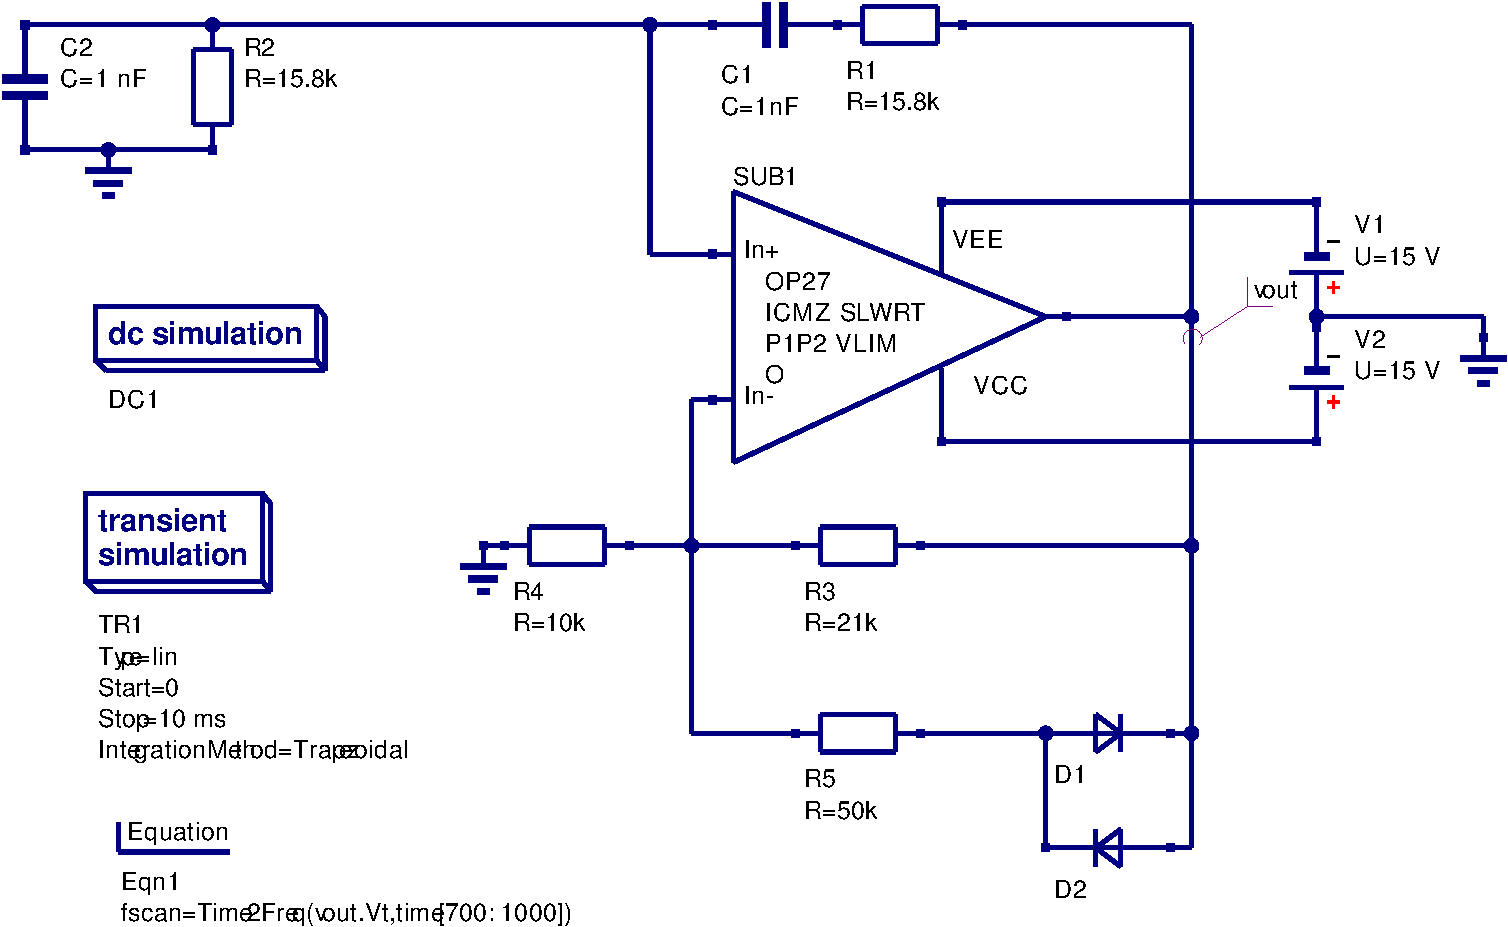
\includegraphics[width=0.9\linewidth]{fig38_sch}
% tcomb1.png: 99.9998dpi, width=11.35cm, height=3.35cm, bb=0 0 447 132
  \caption{Wien bridge oscillator with automatic gain control. } 
  \label{fig:opamp38}
\end{figure}

\begin{figure}
  \centering
  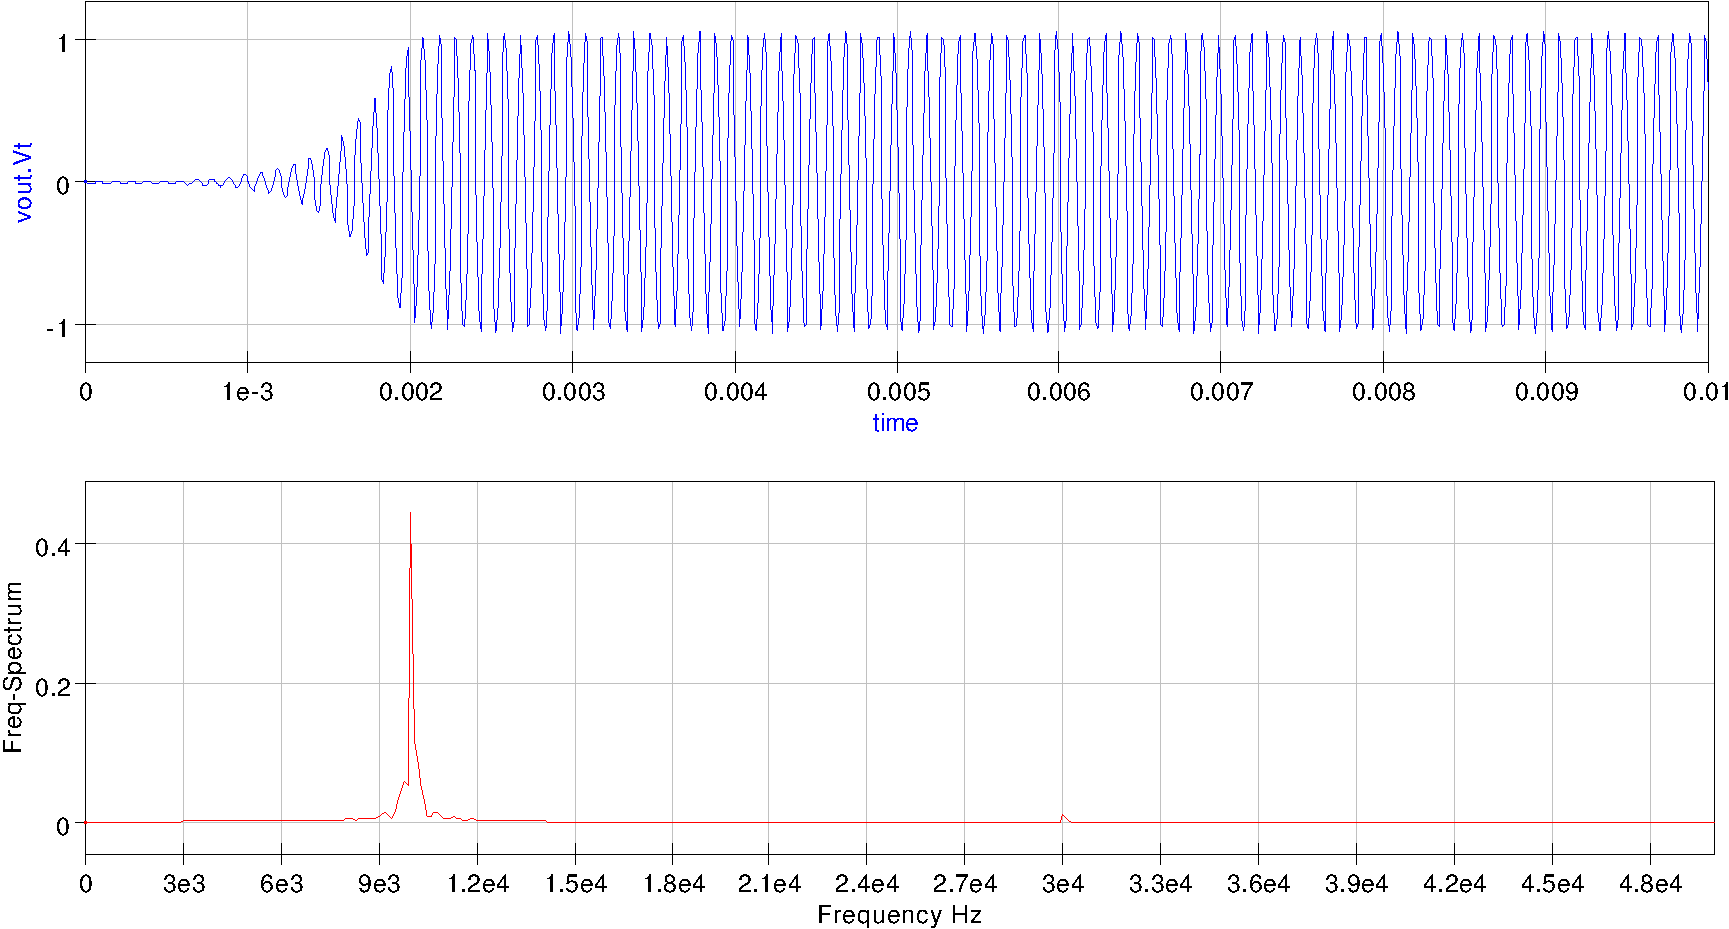
\includegraphics[width=0.9\linewidth]{fig39_dpl}
% tcomb1.png: 99.9998dpi, width=11.35cm, height=3.35cm, bb=0 0 447 132
  \caption{Simulation waveforms for the circuit shown in Fig.~\ref{fig:opamp38}: OP27 AC + slew rate + vlimit macromodel. } 
  \label{fig:opamp39}
\end{figure}

\begin{figure}
  \centering
  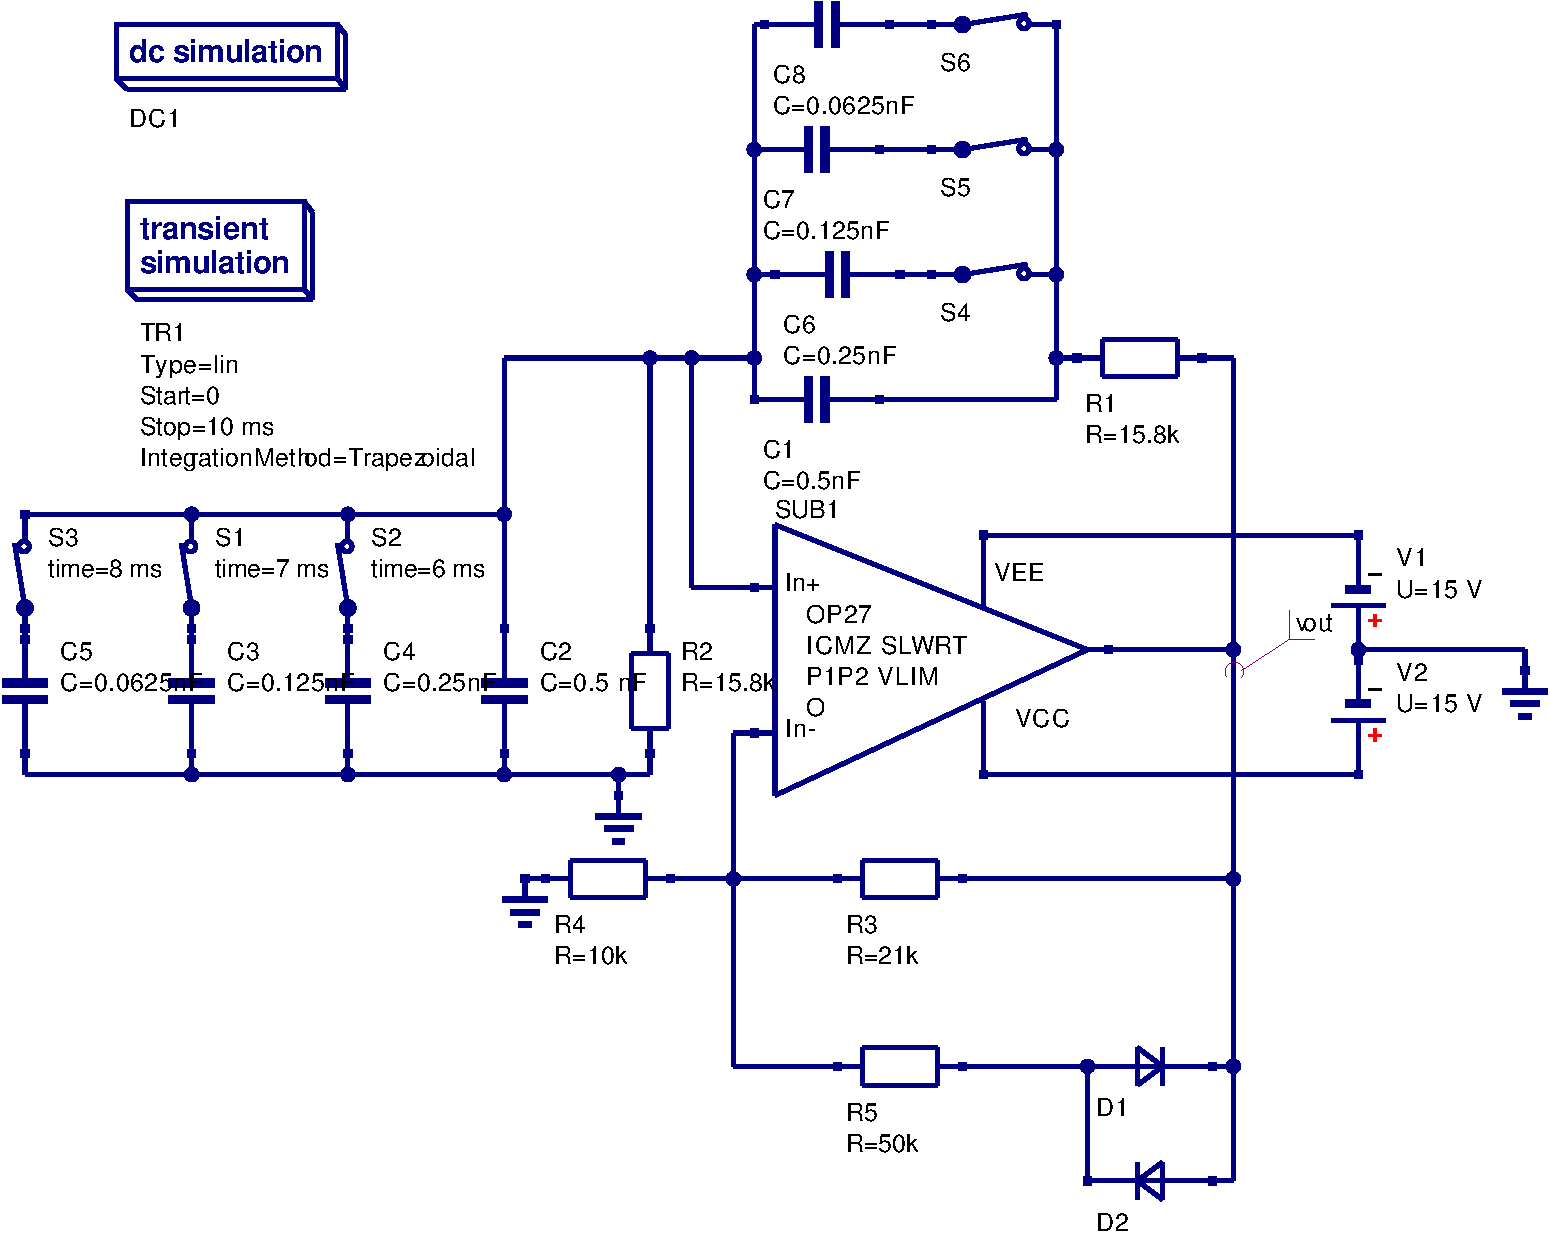
\includegraphics[width=0.9\linewidth]{fig40_sch}
  \caption{Wien bridge oscillator with switched capacitor frequency control. } 
  \label{fig:opamp40}
\end{figure}

\begin{figure} 
  \centering
  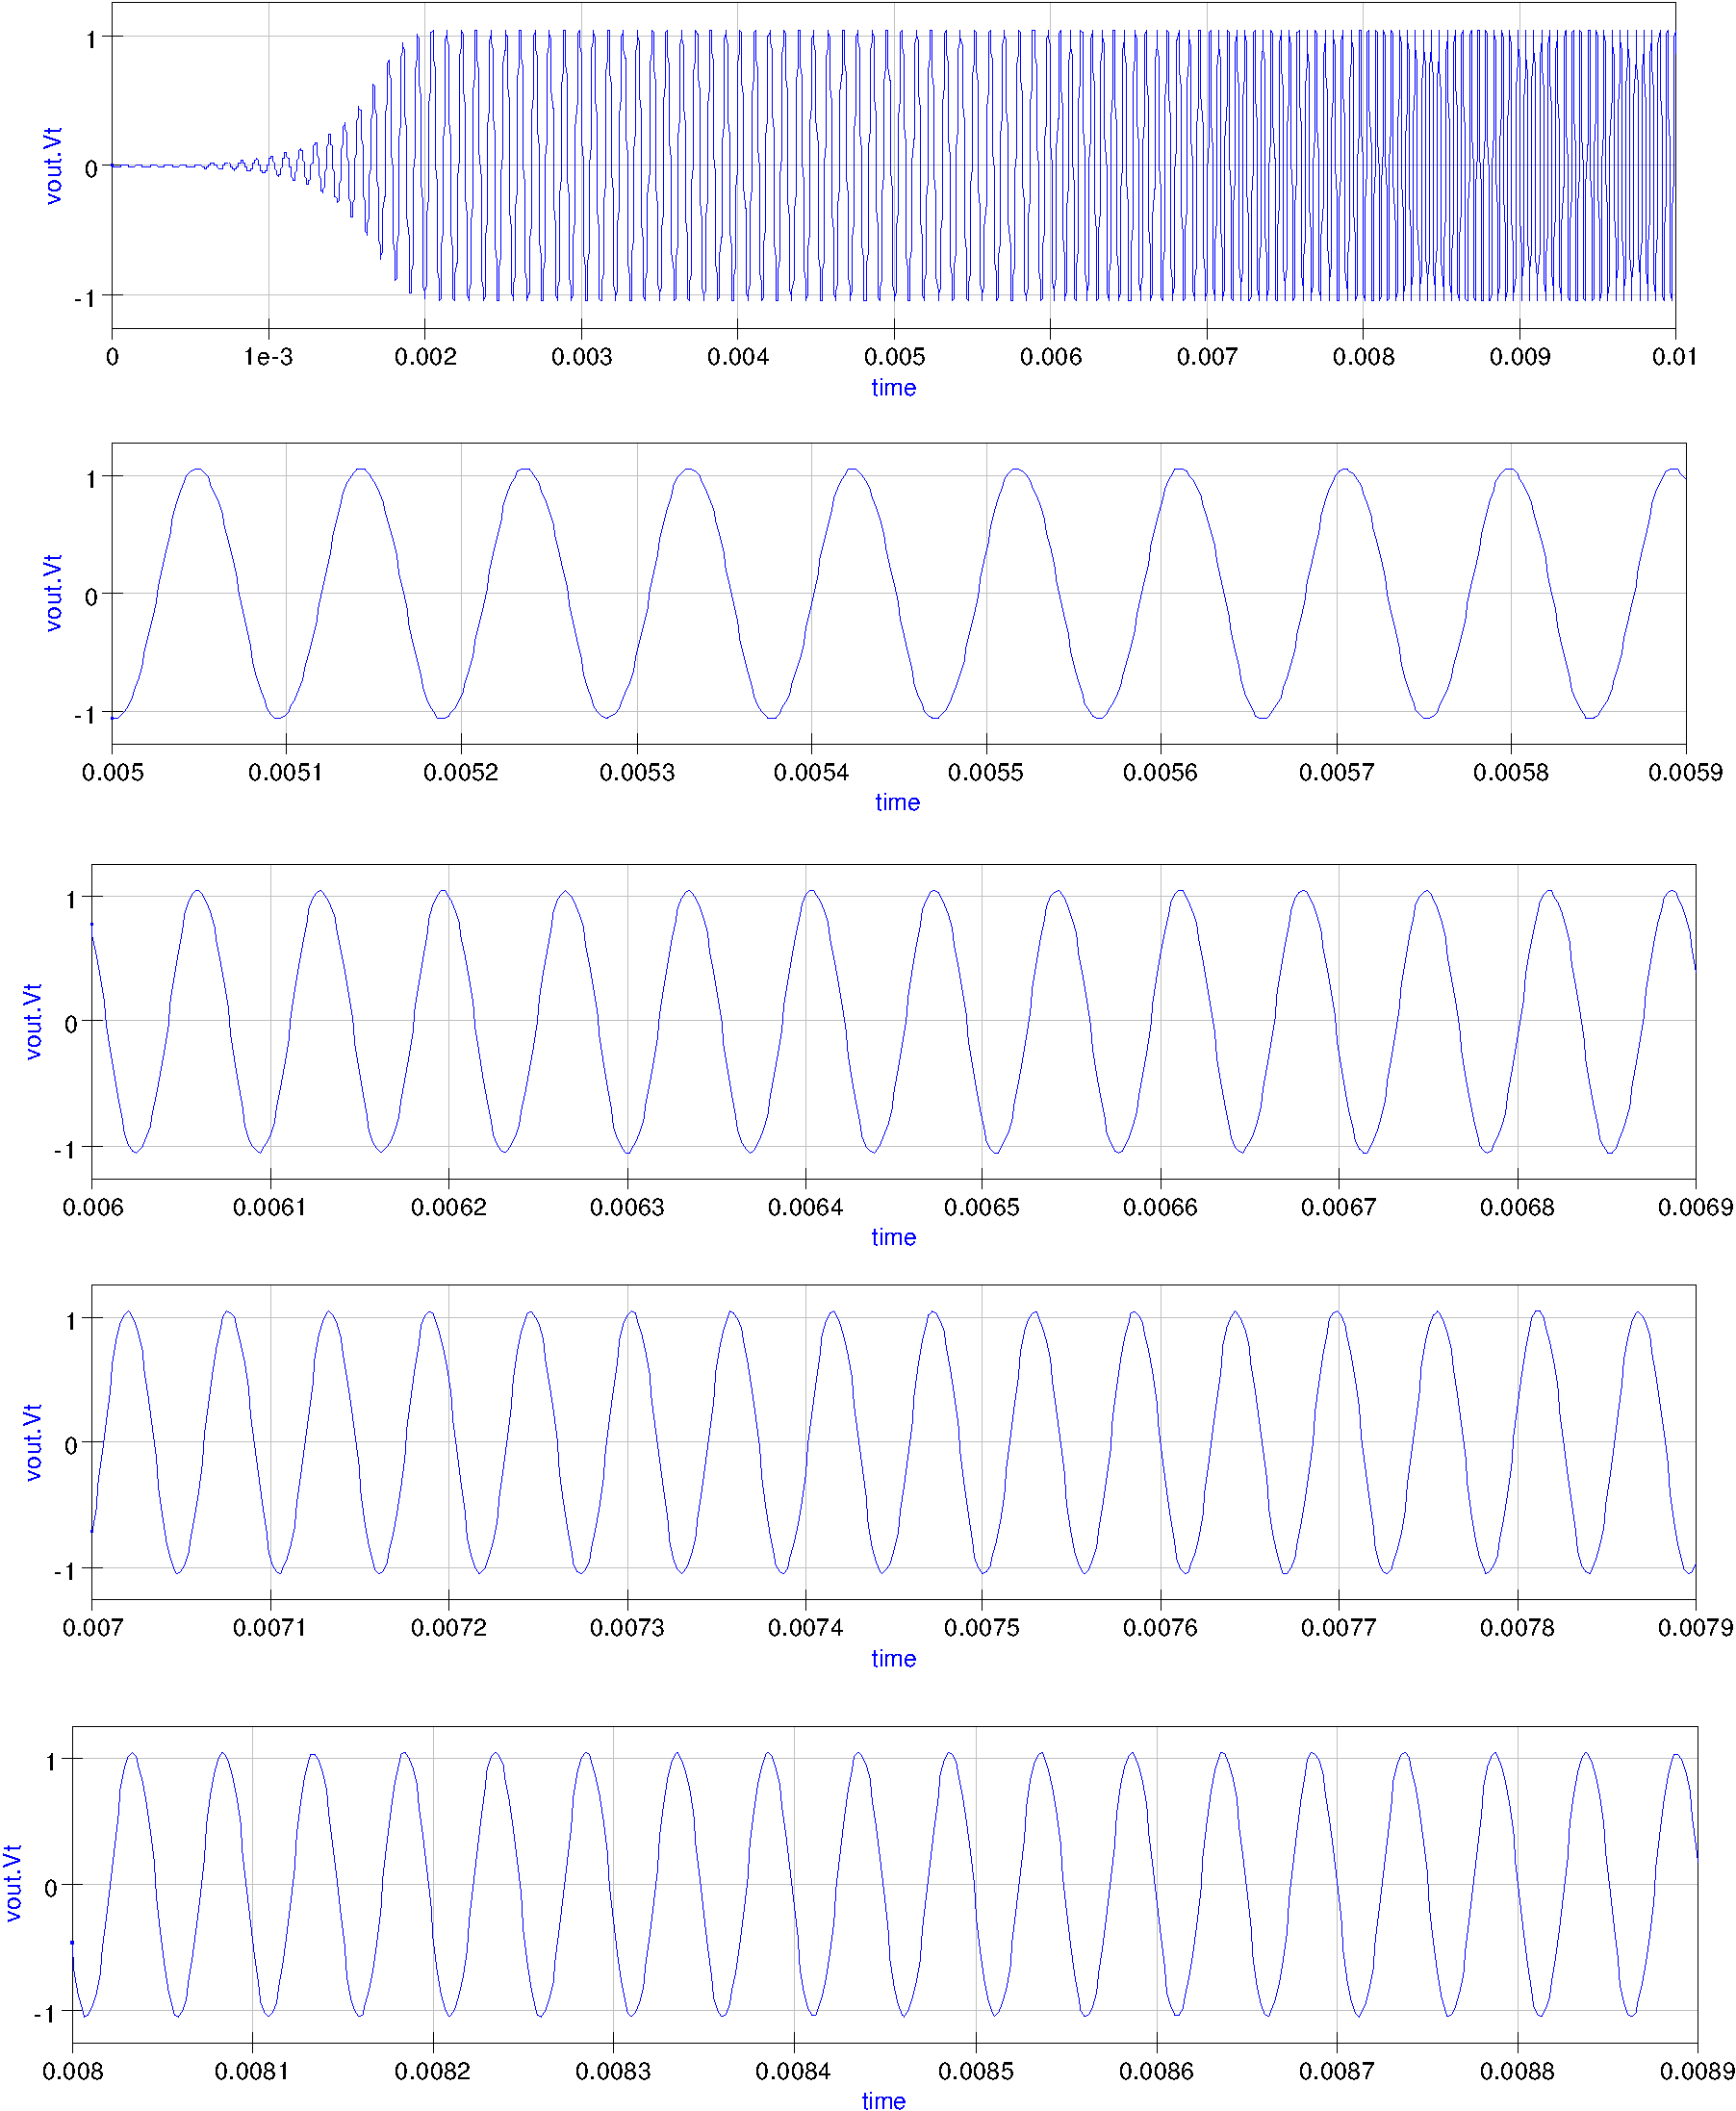
\includegraphics[width=0.9\linewidth]{fig41_dpl}
% tcomb1.png: 99.9998dpi, width=11.35cm, height=3.35cm, bb=0 0 447 132 
  \caption{Simulation waveforms for the circuit shown in Fig.~\ref{fig:opamp40}: OP27 AC + slew rate + vlimit macromodel. } 
  \label{fig:opamp41}
\end{figure}

\tutsection{Update number one: March 2007}
In this first update to the operational amplifier tutorial readers will be introduced to Qucs macromodel model building using schematics and SPICE to Qucs conversion techniques, secondly to procedures for constructing  Qucs operational amplifier libraries, and finally to two different approaches which allow existing OP AMP models to be extended to include new amplifier performance parameters, for example power supply rejection. This update is very much a report on the OP AMP modelling work that has been done by the Qucs development team since version 0.0.10 of the package was released in September 2006.  Future Qucs releases will offer many significant improvements in OP AMP modelling particularly via SPICE to Qucs netlist conversion, subcircuit passing and equation embedding in Qucs schematics  and library development. Following the release of Qucs 0.0.11, and a suitable period of time for new feature debugging, many of the ideas introduced in this update will be developed to include OP AMP model building using embedded equations in Qucs schematics.

\tutsubsection{Building a library component for the modular OP AMP macromodel} 
One of the main strengths of the modular macromodel approach to device modelling is the fact that the parameters implicit in each section of a macromodel are essentially independent, allowing subcircuit blocks to be easily connected together to form an overall device model.  Taking this idea further one can construct a complete schematic for an OP AMP model from the circuitry that represents individual macromodel subcircuit blocks.  The diagram shown in Fig.~\ref{fig:opamp42} illustrates a typical circuit schematic for a modular OP AMP macromodel.  In this schematic the component values are for the UA741 OP AMP.  By attaching a symbol to the modular macromodel schematic the UA741 modular OP AMP model is ready for general use and can be placed in an existing\footnote{Qucs 0.0.10, and earlier releases, were distributed with an OP AMP library called OpAmps. However, this only contained a component level model for the 741 OP AMP. Many of the models discussed in this text have been added to the Qucs OpAmps library. These should assist readers who wish to experiment with their own OP AMP circuits.} or a user defined library.  Moreover, by recalculating the component values further library elements can be constructed and the development of a more extensive Qucs OP AMP library undertaken\footnote{One of the important future tasks is the development of component libraries for use with Qucs - this will take time but should be possible given enough effort by everyone interested in Qucs.}.
 
\begin{figure} 
  \centering
  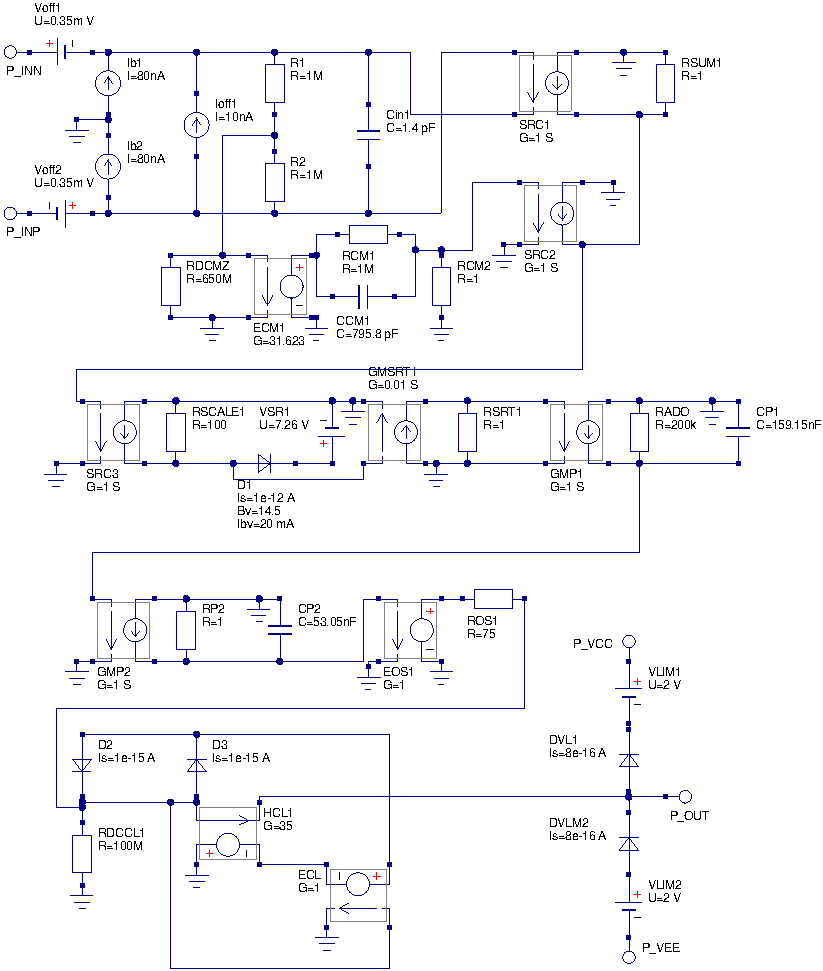
\includegraphics[width=0.9\linewidth]{opamp_fig42}
% tcomb1.png: 99.9998dpi, width=11.35cm, height=3.35cm, bb=0 0 447 132 
  \caption{Modular OP AMP macromodel in schematic form - this model does not include signal overloading. } 
  \label{fig:opamp42}
\end{figure}

\tutsubsection{Changing model parameters: use of the SPICEPP preprocessor}
Changing the component data in Fig.~\ref{fig:opamp42} allows users to generate modular macromodels for different operational amplifiers.  Although this is a perfectly viable approach to model generation it is both tedious and error prone. A more straightforward way is to get the computer to do the tedious work involving component value calculation from device data. With this approach users are only required to enter the device data; as a simple list derived from manufacturers data sheets. One way to do this is to write a SPICE preprocessor template\footnote{The use of the SPICE preprocessors SPICEPP and SPICEPRM are described in Qucs tutorial \textit{Qucs simulation of SPICE netlists}.  Since both SPICEPP and SPICEPRM were first written, Friedrch Schmidt has developed a PSpice to SPICE3/XSPICE preprocessor which combines, and extends, the features found in both SPICEPP and SPICEPRM. This preprocessor is called PS2SP. The Perl script version of PS2SP is licensed under GPL and may be downloaded from http://members.aon.at/fschmid7/. } and let a SPICE preprocessor generate the model for a specific OP AMP. The PS2SP template file for an OP27 OP AMP modular macromodel is given in Fig.~\ref{fig:opamp43}.  The resulting SPICE file is shown in Fig.~\ref{fig:opamp44}. After construction of the SPICE OP27 netlist the Qucs OP27 model is generated via the schematic capture SPICE netlist facility.\footnote{See the tutorial \textit{Qucs simulation of SPICE netlist} for instructions on how this can be done. }

\tutsubsection{The Boyle operational amplifier SPICE model}

The Boyle\footnote{G.R. Boyle, B.M. Cohn, D. Pederson, and J.E. Solomon, Macromodelling of integrated circuit operational amplifiers, IEEE Journal of Solid State Circuits, vol. SC-9, pp. 353-364, 1974.} operational amplifier model was one of the earliest attempts at constructing an OP AMP macromodel that achieved significantly reduced simulation times, when compared to those times obtained with discrete transistor level models\footnote{See Fig.~\ref{fig:opamp3}. Tests show that the Boyle macromodel reduces simulation times for common amplifier, timer and filter circuits by a factor between six and ten.}, while maintaining acceptable functional properties and simulation accuracy. The Boyle macromodel was designed to model differential gain versus frequency, DC common-mode gain, device input and output characteristics, slew rate limiting, output voltage swing and short-circuit limiting.  The circuit schematic for the Boyle macromodel of a bipolar OP AMP  is illustrated in Fig.~\ref{fig:opamp45}. This model consists of three connected stages: the input stage, the intermediate voltage gain stage and the output stage. Calculation of individual component values is complex, relying on a set of equations derived from the physical properties of the semiconductor devices and the structure of the electrical network.  These equations are derived in the Boyle paper and summerised in the following list. Starting with $I_{S1} = $8.0e-16, the emitter base leakage current of transistor T1, and by assuming $R2 = 100k$ the model component values can be calculated using:
\begin{enumerate}
 \item $I_{S2} = I_{S1} \cdot exp\left(\frac{VOS}{Vt}\right)   \cong I_{S1}\left[ 1+\dfrac{VOS}{Vt}\right]$ ,where $Vt = $ 26e-3 V.
 \item $I_{C1} = \dfrac{C_{2} SR^{+}}{2}$, where $SR^{+}$ is the positive slew rate.
 \item $I_{C2} = I_{C1}$
 \item $I_{B1} = I_{B}-\dfrac{I_{OS}}{2}$ and $I_{B2} = I_{B} + \dfrac{I_{OS}}{2}$
 \item $B_{1} = \dfrac{I_{C1}}{I_{B1}}$ and $B_{2} = \dfrac{I_{C2}}{I_{B2}}$ 
 \item $IEE = \left[ \dfrac{B_{1}+1}{B_{1}} + \dfrac{B_{2}+1}{B_{2}}\right] I_{C1}$
 \item $RC1 = \dfrac{1}{2 \pi GBP C_{2}}$ 
 \item $RC2 = RC1$
 \item $RE1 = \dfrac{B_{1}+B_{2}}{2+B_{1}+B_{2}}\left[ RC1-\dfrac{1}{gm1}\right] $, where $gm1 = \dfrac{I_{C1}}{Vt}$, and $RE2 = RE1$
 \item $CEE = \dfrac{C2}{2} \cdot tan\left(  \triangle \phi \dfrac{\pi}{180}\right)$, where $\triangle \phi = 90^{o} - \Phi m$ and $\Phi m$ is the phase margin.
 \item $GCM = \dfrac{1}{CMMR RC1}$
 \item $GA = \dfrac{1}{RC1}$
 \item $GB = \dfrac{AvOL RC1}{R2 RO2}$
 \item $ISD1 = IX \cdot exp\left(TMP1\right) $+1e-32, where $IX = 2 \cdot I_{C1} \cdot R2 \cdot GB -I_{S1}$, \linebreak and $TMP1 = \dfrac{-1}{RO1\dfrac{I_{S1}}{Vt}}$
 \item $RC = \dfrac{Vt}{100 \cdot IX}ln\left( TEMP2\right) $, where $TEMP2 = \dfrac{IX}{ISD1}$
 \item $VC = abs\left( VCC\right) - VOUT_P + Vt \cdot ln\left( \dfrac{ISC_P}{I_{S1}}\right) $
 \item $VE = abs\left( VEE\right) + VOUT_N + VT \cdot ln\left( \dfrac{ISC_N}{I_{S1}}\right) $ 
 \item $RP = \dfrac{\left( VCC-VEE\right) \left( VCC-VEE\right) }{PD}$
\end{enumerate}

Rather than calculate the Boyle macromodel component values by hand using a calculator it is better to use a PS2SP preprocessor template that does these calculations and also generates the Boyle SPICE netlist. A template for this task is given in Fig.~\ref{fig:opamp46}.  The parameters at the beginning of the listing are for the UA741 OP AMP. In Fig.~\ref{fig:opamp46} the macromodel internal nodes are indicated by numbers and external nodes by descriptive names. This makes it easier to attach the macromodel interface nodes to a Qucs schematic symbol.  The SPICE netlist shown in Fig.~\ref{fig:opamp47} was generated by SP2SP.

\begin{figure} 
\begin{lstlisting}[
 language=Clean, 
 basicstyle=\scriptsize]
*subcircuit ports: in+   in-   p_out  p_vcc p_vee 
.subckt opamp_ac in_p in_n p_out p_vcc p_vee
* OP27 OP AMP parameters
.param voff = 30.0u  ib = 15n  ioff = 12n
.param rd = 4meg  cd = 1.4p  cmrrdc = 1.778e6
.param fcmz = 2000.0 aoldc = 1.778e6  gbp = 8meg
.param fp2 = 17meg  pslewr=2.8e6  nslewr=2.8e6
.param vccm=15  vpoutm=14  veem=-15
.param vnoutm=-14  idcoutm=32m  ro=70.0
.param p1={(100*pslewr)/(2*3.1412*gbp) -0.7}
.param p2={(100*nslewr)/(2*3.1412*gbp) -0.7}
* input stage 
voff1 in_n 6 {voff/2}
voff2 7 in_p {voff/2}
ib1   0 6 {ib}
ib2   7 0 {ib}
ioff1 7 6 {ioff/2}
r1    6 8 {rd/2}
r2    7 8 {rd/2}
cin1  6 7 {cd}
* common-mode zero stage
ecm1 12 0 8 0 {1e6/cmrrdc}
rcm1 12 13 1meg
ccm1 12 13 {1/(2*3.1412*1e6*fcmz)}
rcm2 13 0 1
* differential and common-mode signal summing stage
gmsum1 0 14 7 6 1
gmsum2 0 14 13 0 1
rsum1  14 0 1
* slew rate stage
gsrc1 0 15 13 0 1
rscale1 15 0 100
dsl 15 16 {dslewrate}
.model dslewrate d(is=1e-12 bv= { p1+p2 } )
vsr1 16 0 {p1}
gmsrt1 0 17 15 0 0.01
rsrt1 17 0 1
* voltage gain stage 1 
gmp1 0 9 17 0 1
rado 9 0 {aoldc}
cp1 9 0 {1/(2*3.1412*gbp)}
* voltage gain stage 2 
gmp2 0 11 9 0 1
rp2  11 0 1
cp2  11 0 {1/(2*3.1412*fp2)}
* output stage 
eos1 10 0 11 0 1
ros1 10 50 {ro}
*output current limiter stage
rdcl1 50 0 100meg
dcl1 21 50 dclim
dcl2 50 21 dclim 
.model dclim d(is=1e-15 cj0=0.0)
vcl1 50 p_out 0v
hcl1 0 22 vcl1 {0.9/idcoutm}
ecl1 21 22 50 0 1
* voltage limiting stage
dvl1 p_out 30 dvlimit
.model dvlimit d(is=8e-16)
dvl2 40 p_out dvlimit
vlim1 p_vcc 30 {vcc-vccm+1}
vlim2 40 p_vee {-vee +veem+1}
.ends
.end

\end{lstlisting}
  \caption{PS2SP template for the OP27 modular macromodel. } 
  \label{fig:opamp43}
\end{figure}

\begin{figure} 
\begin{lstlisting}[
 language=Clean, 
 basicstyle=\scriptsize]
*subcircuit ports: in+ in- p_out p_vcc p_vee
* infile=op27.pp date=Tue Feb 13 17:32:37 2007 Converted with ps2sp.pl V4.11
* options: -sp3=0 -ltspice=0 -fromsub=0 -fromlib=0 -check=0 (tinylines=1)
* copyright 2007 by Friedrich Schmidt - terms of Gnu Licence
.subckt opamp_ac in_p in_n p_out p_vcc p_vee
voff1 in_n 6 1.5e-05
voff2 7 in_p 1.5e-05
ib1 0 6 1.5e-08
ib2 7 0 1.5e-08
ioff1 7 6 6e-09
r1 6 8 2000000
r2 7 8 2000000
cin1 6 7 1.4e-12
ecm1 12 0 8 0 0.562429696287964
rcm1 12 13 1meg
ccm1 12 13 7.95874188208328e-11
rcm2 13 0 1
gmsum1 0 14 7 6 1
gmsum2 0 14 13 0 1
rsum1 14 0 1
gsrc1 0 15 13 0 1
rscale1 15 0 100
dsl 15 16 0
.model dslewrate d(is=1e-12 bv= 9.7422386349166 )
vsr1 16 0 4.8711193174583
gmsrt1 0 17 15 0 0.01
rsrt1 17 0 1
gmp1 0 9 17 0 1
rado 9 0 1778000
cp1 9 0 1.98968547052082e-08
gmp2 0 11 9 0 1
rp2 11 0 1
cp2 11 0 9.36322574362739e-09
eos1 10 0 11 0 1
ros1 10 50 70
rdcl1 50 0 100meg
dcl1 21 50 dclim
dcl2 50 21 dclim
.model dclim d(is=1e-15 cj0=0.0)
vcl1 50 p_out 0v
hcl1 0 22 vcl1 28.125
ecl1 21 22 50 0 1
dvl1 p_out 30 dvlimit
.model dvlimit d(is=8e-16)
dvl2 40 p_out dvlimit
vlim1 p_vcc 30 -14
vlim2 40 p_vee -14
.ends
.end
\end{lstlisting}
  \caption{SPICE netlist for the OP27 modular macromodel. }  
  \label{fig:opamp44}
\end{figure}


\begin{figure} 
  \centering
  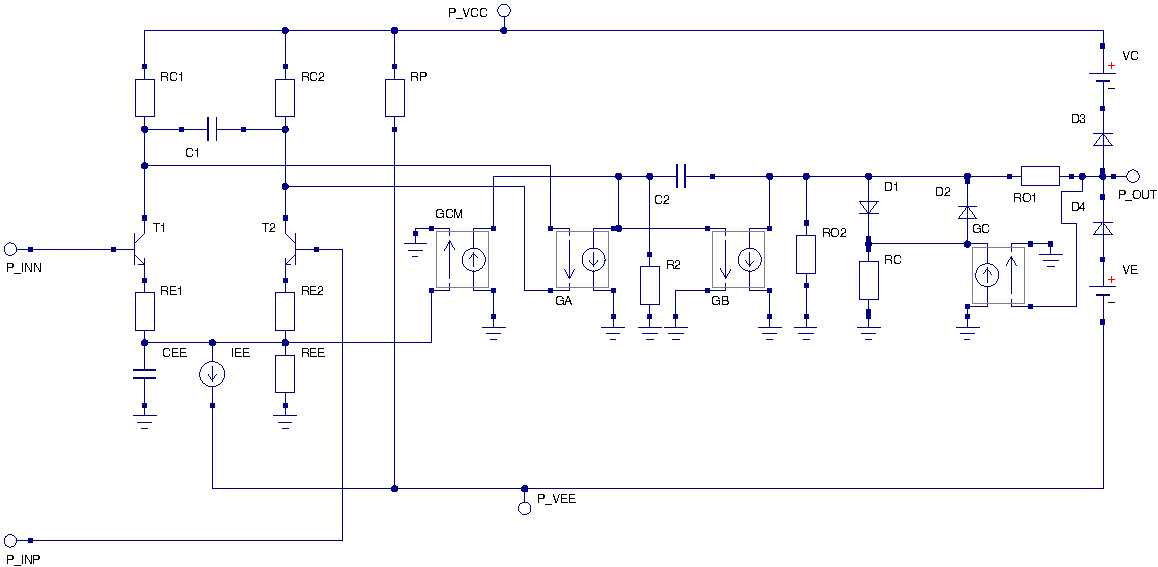
\includegraphics[width=1.0\linewidth]{fig44_sch}
% tcomb1.png: 99.9998dpi, width=11.35cm, height=3.35cm, bb=0 0 447 132 
  \caption{Boyle macromodel for a BJT OP AMP } 
  \label{fig:opamp45}
\end{figure}

\begin{figure} 
  \centering
\begin{lstlisting}[
 language=Clean, 
 basicstyle=\scriptsize]

* Boyle macromodel template for Qucs.
* Design parameters (For UA741)
.param vt=26e-3  $ Thermal voltage at room temp.
.param c2=30e-12    $ Compensation capacitance
.param positive_slew_rate=0.625e6 negative_slew_rate=0.50e6  $ Slew rates
.param is1=8.0e-16  $ T1 leakage current
.param vos=0.7e-3 ib=80n ios=20n  $ Input voltage and current parameters
.param va=200  $ Nominal early voltage
.param gbp=1.0e6 $ Gain bandwidth product
.param pm=70 $ Excess phase at unity gain.
.param cmrr=31622.8 $ Common-mode rejection ratio (90 dB)
.param avol=200k $ DC open loop differential gain
.param ro2=489.2 $ DC output resistance
.param ro1=76.8 $ High frequency AC output resistance
.param r2=100k
.param vout_p=14.2 $ Positive saturation voltage - for VCC=15v
.param vout_n=-13.5 $ Negative saturation voltage - for VCC=-15v
.param vcc=15 $ Positive power supply voltage
.param vee=-15 $ Negative power supply voltage
.param isc_p=25m $ Short circuit output current
.param isc_n=25m $ Short circuit output current
.param pd=59.4m $ Typical power dissipation
* Design equations
.param is2={is1*(1+vos/vt)}
.param ic1={0.5*c2*positive_slew_rate} ic2={ic1}
.param ib1={ib-0.5*ios} ib2={ib+0.5*ios}
.param b1={ic1/ib1} b2={ic2/ib2}
.param iee={((b1+1)/b1+(b2+1)/b2)*ic1}
.param gm1={ic1/vt} rc1={1/(2*3.1412*gbp*c2)} rc2=rc1
.param re1={((b1+b2)/(2+b1+b2))*(rc1-1/gm1)} re2=re1
.param ree={va/iee} cee={(2*ic1/negative_slew_rate)-c2}
.param dphi={90-pm} c1={(c2/2)*tan(dphi*3.1412/180)}
.param gcm={1/(cmrr*rc1)} ga={1/rc1} gb={(avol*rc1)/(r2*ro2)}
.param ix={2*ic1*r2*gb-is1} tmp1={-1.0/(ro1*is1/vt)} isd1={ix*exp(tmp1)+1e-32}
.param tmp2={ix/isd1} rc={vt/(100*ix)*ln(tmp2)}
.param gc={1/rc}
.param vc={abs(vcc)-vout_p+vt*ln(isc_p/is1)} ve={abs(vee)+vout_n+vt*ln(isc_n/is1)}
.param rp={(vcc-vee)*(vcc-vee)/pd}
* Nodes: Input n_inp n_inn n_vcc n_vee   Output n_out
Q1 8 n_inn 10 qmod1
Q2 9 n_inp 11 qmod2
RC1 n_vcc 8 {rc1}
RC2 n_vcc 9 {rc2}
RE1 1 10 {re1}
RE2 1 11 {re2}
RE 1 0 {ree}
CE 1 0 {cee}
IEE 1 n_vee {iee}
C1 8 9 {c1}
RP n_vcc n_vee {rp}
GCM 0 12 1 0 {gcm}
GA 12 0 8 9 {ga}
R2 12 0 {r2}
C2 12 13 30p
GB 13 0 12 0 {gb}
RO2 13 0 {ro2}
RO1 13 n_out {ro1}
D1 13 14 dmod1
D2 14 13 dmod1
GC 0 14 n_out 0 {gc}
RC 14 0 {rc}
D3 n_out 15 DMOD3
D4 16 n_out DMOD3
VC n_vcc 15 {vc}
VE 16 n_vee {ve}
.model dmod1 d(is={isd1} rs=1)
.model dmod3 d(is=8e-16 rs=1)
.model qmod1 npn(is={is1} BF={b1})
.model qmod2 npn(is={is2} BF={b2})
.end
\end{lstlisting}
  \caption{PS2SP template for the Boyle macromodel with UA741 parameters listed. } 
  \label{fig:opamp46}
\end{figure}

\begin{figure} 
  \centering
\begin{lstlisting}[
 language=Clean, 
 basicstyle=\scriptsize]
* boyle macromodel template for qucs.
* infile=ua741_boyle.ps2sp date=Tue Feb 6 20:58:12 2007 Converted with ps2sp.pl V4.11
* options: -sp3=0 -ltspice=0 -fromsub=0 -fromlib=0 -check=0 (tinylines=1)
* copyright 2007 by Friedrich Schmidt - terms of Gnu Licence
q1 8 n_inn 10 qmod1
q2 9 n_inp 11 qmod2
rc1 n_vcc 8 5305.82792138885
rc2 n_vcc 9 5305.82792138885
re1 1 10 1820.05072213971
re2 1 11 1820.05072213971
re 1 0 13192612.1372032
ce 1 0 7.5e-12
iee 1 n_vee 1.516e-05
c1 8 9 5.4588124089082e-12
rp n_vcc n_vee 15151.5151515152
gcm 0 12 1 0 5.96000354174836e-09
ga 12 0 8 9 0.000188472
r2 12 0 100000
c2 12 13 30p
gb 13 0 12 0 21.6918557701915
ro2 13 0 489.2
ro1 13 n_out 76.8
d1 13 14 dmod1
d2 14 13 dmod1
gc 0 14 n_out 0 1621.78603105575
rc 14 0 0.000616604151750539
d3 n_out 15 dmod3
d4 16 n_out dmod3
vc n_vcc 15 1.60789905279489
ve 16 n_vee 2.30789905279488
.model dmod1 d(is=1e-32 rs=1)
.model dmod3 d(is=8e-16 rs=1)
.model qmod1 npn(is=8e-16 bf=107.142857142857)
.model qmod2 npn(is=8.21538461538461e-16 bf=83.3333333333333)
.end
\end{lstlisting}
  \caption{SPICE netlist for the Boyle UA741 macromodel. } 
  \label{fig:opamp47}
\end{figure}


\tutsubsection{Model accuracy}
The modular and Boyle OP AMP macromodels are examples of typical device models in common use with todays popular circuit simulators. A question which often crops up is which model is best to use when simulating a particular circuit? This is a complex question which requires careful consideration. One rule of thumb worth following is \textbf{always validate a SPICE/Qucs model before use}. Users can then check that a specific model does simulate the circuit parameters that control the function and accuracy of the circuit being designed\footnote{An interesting series of articles by Ron Mancini, on verification and use of SPICE models in circuit design can be found in the following editions of EDN magazine:Validate SPICE models before use, EDN March 31, 2005 p.22; Understanding SPICE models, EDN April 14, p 32; Verify your ac SPICE model, EDN May 26, 2005; Beyond the SPICE model's dc and ac performance, EDN June 23 2005, and Compare SPICE-model performance, EDN August 18, 2005.}. One way to check the performance of a given model is to simulate a specific device parameter.  The simulation results can then be compared to manufacturers published figures and the accuracy of a model easily determined.  By way of an example consider the simulation circuit shown in Fig.~\ref{fig:opamp48}.  In this circuit the capacitors and inductors ensure that the devices under test are in ac open loop mode with stable dc conditions.  Figure~\ref{fig:opamp49} illustrates the observed simulation gain and phase results for four different OP AMP models.  Except at very high frequencies, which are outside device normal operating range, good agreement is found between manufacturers data and that recorded by the open loop voltage gain test for both the modular and Boyle macromodels.

\begin{figure} 
  \centering
  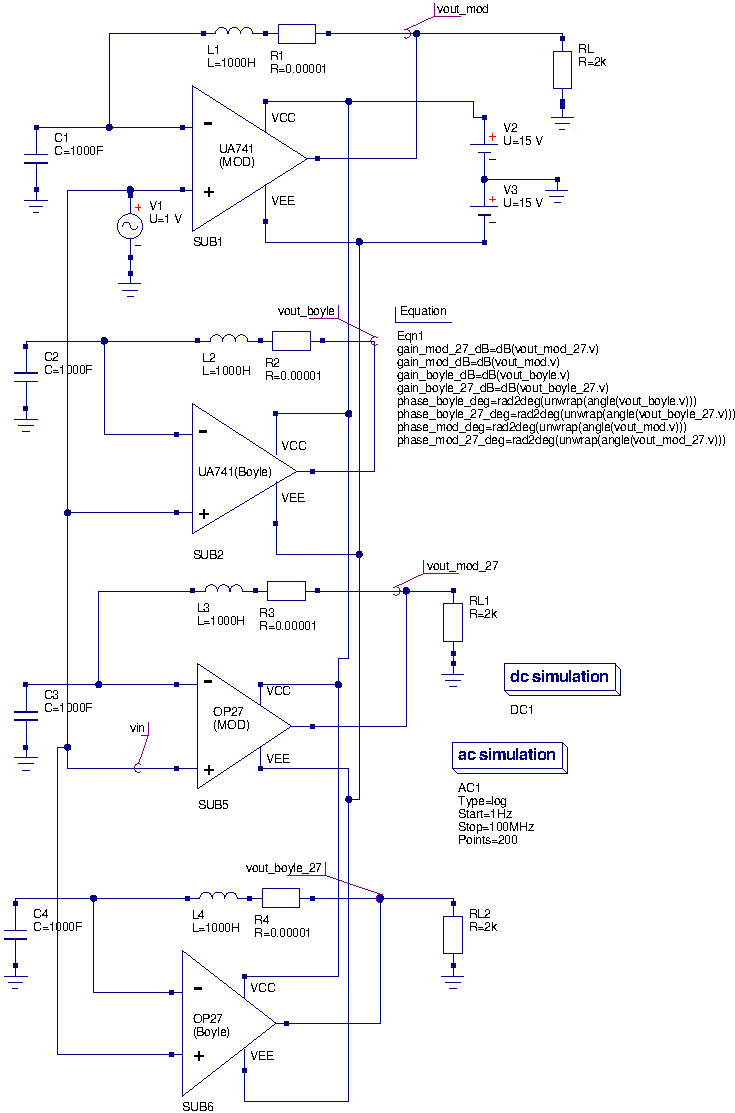
\includegraphics[width=0.8\linewidth]{opamp_fig48}
% tcomb1.png: 99.9998dpi, width=11.35cm, height=3.35cm, bb=0 0 447 132 
  \caption{Test circuit for simulating OP AMP model open loop voltage gain. }  
  \label{fig:opamp48}
\end{figure}

\begin{figure} 
  \centering
  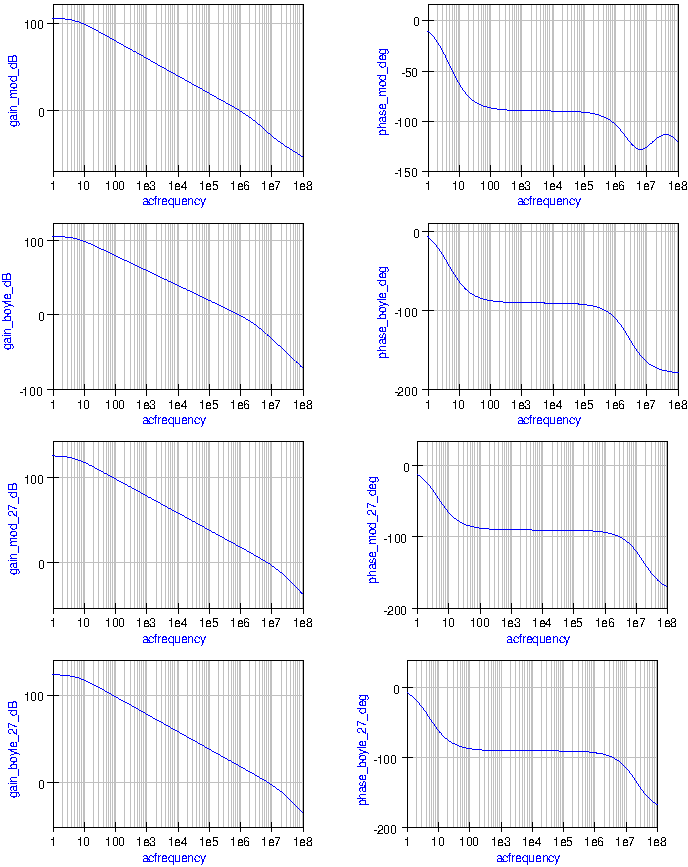
\includegraphics[width=0.8\linewidth]{opamp_fig49}
% tcomb1.png: 99.9998dpi, width=11.35cm, height=3.35cm, bb=0 0 447 132 
  \caption{ Open loop voltage gain simulation waveforms for the modular and Boyle UA741 and OP27 macromodels. }  
  \label{fig:opamp49}
\end{figure}



\tutsubsection{The PSpice modified Boyle model}
One of the most widely used OP AMP simulation models is a modified version of the Boyle macromodel.  This was originally developed for use with the PSpice circuit simulator. Many semiconductor manufacturers provide models for their devices based on the modified Boyle macromodel\footnote{See for example the OP AMP section of the Texas Instruments (TI) Web site and the TI Operational Amplifier Circuits, Linear Circuits, Data Manual, 1990.}. A typical modified Boyle macromodel SPICE netlist is shown in Fig.~\ref{fig:opamp50}. The circuit structure and performance are very similar, but significantly different to the original Boyle model. Some of the common OP AMP parameters NOT modeled are (1) input offset voltage, (2) temperature coefficient of input offset voltage, (3) input offset current, (4) equivalent input voltage and noise currents, (5) common-mode input voltage range, and (6) temperature effect on component stability. Items (2), (4), (5) and (6) are also not modeled by the standard Boyle macromodel. Although the modified Boyle macromodel is similar to the original Boyle model it is not possible to use this model as it is defined with Qucs; due to the fact that SPICE 2G nonlinear controlled sources, egnd and fb, are included in the SPICE netlist. Controlled source egnd is employed to model the OP AMP reference voltage as the average of the VCC and VEE power rail voltages rather than the ground voltage assumed in the original Boyle macromodel\footnote{Taking the OP AMP reference voltage to be the average of VCC and VEE allows devices with non-symmetrical power supply voltages to be simulated.}. Current conrolled current source fb is used to model OP AMP output current limiting. The nonlinear polynomial\footnote{The definition of these polynomial functions was changed in the SPICE 3 series simulators to a more conventional algebraic form when specifying the B type source components.  This often gives compatibility problems when attempting to simulate SPICE 2 models with circuit simulators developed from SPICE 3f4 or earlier simulators. Most popular SPICE based circuit simulators now accept both types of nonlinear syntax.} form of controlled sources were included in the 2G series of SPICE simulators to allow behavioural models of summers, multipliers, buffers and other important functional components to be easily constructed. Single and multidimensional polynomial forms of controlled sources are defined by SPICE 2G. Taking (1) the voltage controlled voltage source and (2) the current controlled current sources as examples the syntax is as follows:

\smallskip 

\verb|Ename N(+) N(-) POLY(n) NC1(+) NC1(-) NC2(+) NC2(-)..... P0  P1  P2......,| \linebreak where n indicates the order of the polynomial with coefficients P0 .....Pn, and NCn(+), NCn(-) etc are the control node pairs.
  
This becomes:
\begin{itemize}
 \item \begin{footnotesize}\verb|For POLY(1)|                         \end{footnotesize}\footnote{ If only one P coefficient is given in the single dimension polynomial case, then SPICE assumes that this is P1 and that P0 equals zero. Similarly if the POLY keyword is not explicitly stated in a controlled source definition then it is assumed by SPICE to be POLY(1).}\begin{footnotesize}\verb|: Ename N(+) N(-) P0 P1 P2.........|                                                                                                                                                                                                                                                                                                                                                          \end{footnotesize}
 \item \begin{footnotesize}\verb|For POLY(2): Ename N(+) N(-) POLY(2) NC1(+) NC1(-) NC2(+) NC(-) P0 P1 P2......|                                                                                            \end{footnotesize}
 \item \begin{footnotesize}\verb|For POLY(3): Ename N(+) N(-) POLY(3) NC1(+) NC1(-) NC2(+) NC2(-) NC3(+) NC3(-) P0 P1 P2....                                                                                              |\end{footnotesize}, and so on.
\end{itemize}            



Similarly:
\begin{footnotesize}Fname N(+) N(-) POLY(n) V1 V2 V3 ...... P0 P1 P2 ....., where V1, V2 .... are independent voltage sources whose current controls the output.
\end{footnotesize}
This becomes:
\begin{itemize}
 \item \begin{footnotesize}For POLY(1): Fname N(+) N(-) V1 P0 P1 P2........
 \item For POLY(2): Fname N(+) N(-) POLY(2) V1 V2 P0 P1 P2.......
 \item For POLY(3): Fname N(+) N(-) POLY(3) V1 V2 V3 P0 P1 P2 P3......., and so on.                                                                    \end{footnotesize}
\end{itemize}


The meaning of the coefficients in the nonlinear controlled source definitions depends on the dimension of the polynomial. The following examples indicate how SPICE calculates current or voltage values.
\begin{itemize}
 \item For POLY(1): The polynomial function $fv$ is calculated using\linebreak 
$fv=P0+(P1*fa)+(P2*fa^{2})+(P3*fa^{3})+(P4*fa^{4})+.........$, \linebreak where $fa$ is either a voltage or current independent variable.
 \item For POLY(2): The polynomial function $fv$ is calculated using\linebreak 
$fv=P0+(P1*fa)+(P2*fb)+(P3*fa^{2})+(P4*fa*fb)+(P5*fb^{2})+(P6*fa^{3})$ 
$+(P7*fa^{2}*fb)+..........$, where $fa$ and $fb$ are both either voltage or current independent variables.
\item For POLY(3): The polynomial function $fv$ is calculated using\linebreak 
$fv=P0+(P1*fa)+(P2*fb)+(P3*fc)+(P4*fa^{2})+(P5*fa*fb)$
$+(P6*fa*fc)+(P7*fb^{2})+(P8*fb*fc)+(P9*fc^{2})+(P10*fa^{3})$
$+(P11*fa^{2}*fb)+(P12*fa^{2}*fc)+(P13*fa*fb^{2})+(P14*fa*fb*fc)$
$+(P15*fa*fc^{2})+(P16*fb^{3})+(P17*fb^{2}*fc)+(P18*fb*fc^{2})$
$+(P19*fc^{3}).............$, where $fa$, $fb$, and $fc$ are all either voltage or current independent variables.
\end{itemize}

From Fig.~\ref{fig:opamp50} the controlled generators egnd and fb are:
 
\begin{itemize}
 \item \verb|egnd 99  0 poly(2) (3,0) (4,0) 0 .5 .5| \linebreak Which is the same as \verb|egnd 99 0 poly(2) 3 0 4 0 0 0.5 0.5| \linebreak By comparison with the SPICE polynomial equations for controlled sources, \linebreak $V(egnd) = \dfrac{V(3)}{2}+\dfrac{V(4)}{2}$  implying that the controlled voltage source $V(egnd)$ is the sum of two linear voltage sources. 

 \item \verb|fb 7 99 poly(5) vb vc ve vlp vln 0 10.61E6 -10E6 10E6 10E6 -10E6| \linebreak  By comparison with the SPICE polynomial equations for controlled sources \linebreak \verb|I(fb) = 10.61e6*I(vb) - 10e6*I(vc) + 10e6*I(ve) + 10e6*I(vlp) -10e6*I(vlp)| implying that the controlled current $I(fb)$ is the sum of five linear controlled current sources.
\end{itemize}

SPICE sources engd and fb can therefore be replaced in the modified Boyle model by the following SPICE code\footnote{It is worth noting that the code for the polynomial form of controlled sources can only be replaced by a series connection of linear controlled voltage sources or a parallel connection of linear controlled current sources provided no higher order polynomial coefficients are present in the original SPICE code.  Some SPICE models use these higher order coefficients to generate multiply functions.  Such cases cannot be converted to code which will simulate using Qucs 0.0.10. Sometime in the future this restriction will be removed when nonlinear voltage and current sources are added to Qucs.}:

\begin{verbatim}

* egnd 99  0 poly(2) (3,0) (4,0) 0 .5 .5
* Forms voltage source with output
* V=0.5*V(4)+0.5*V(3)
egnd1 999 0 4 0 0.5
egnd2 99 999 3 0 0.5
*
*fb 7 99 poly(5) vb vc ve vlp vln 0 10.61e6 -10e6 10e6 10e6 -10e6
*
* Forms current source with output
* I=10.61e6*i(vb)-10e6*i(vc)+10e6*i(ve)+10e6*i(vlp)-10e6*i(vln)
*
*Sum 5 current sources to give fb.
fb1 7 99 vb 10.61e6
fb2 7 99 vc -10e6
fb3 7 99 ve 10e6
fb4 7 99 vlp 10e6
fb5 7 99 vln -10e6
\end{verbatim} 

Modified Boyle macromodels are often generated using the PSpice Parts\footnote{The Parts modelling program is an integral component in the PSpice circuit simulation software originally developed by the MicroSim Corporation, 1993, The Design Centre:Parts (Irvine, Calif.). It now forms part of Cadence Design Systems OrCad suite of CAD software.} program.  Such models have similar structured SPICE netlists with different component values. However, changes in technology do result in changes in the input stage that reflect the use of npn, pnp and JFET input transistors in real OP AMPs.  Hence to use manufacturers published modified Boyle models with Qucs all that is required is the replacement of the SPICE polynomial controlled sources with linear sources and the correct component values. Again this is best done using a SPICE preprocessor template. The templates for OP AMPS with npn and PJF input transistors are shown in Figures ~\ref{fig:opamp51} and ~\ref{fig:opamp52}. The SPICE netlists shown in Figs.~\ref{fig:opamp53} and ~\ref{fig:opamp54} were generated by the PS2SP preprocessor.  For OP AMPS with pnp input transistors simply change the BJT model reference from npn to pnp and use the same template. 
\begin{figure} 
  \centering
\begin{lstlisting}[
 language=Clean, 
 basicstyle=\scriptsize]

* connections:   non-inverting input
*                |  inverting input
*                |  |  positive power supply
*                |  |  |  negative power supply
*                |  |  |  |  output
*                |  |  |  |  |
.subckt uA741    1  2  3  4  5
*
  c1   11 12 8.661E-12
  c2    6  7 30.00E-12
  dc    5 53 dx
  de   54  5 dx
  dlp  90 91 dx
  dln  92 90 dx
  dp    4  3 dx
  egnd 99  0 poly(2) (3,0) (4,0) 0 .5 .5
  fb    7 99 poly(5) vb vc ve vlp vln 0 10.61E6 -10E6 10E6 10E6 -10E6
  ga    6  0 11 12 188.5E-6
  gcm   0  6 10 99 5.961E-9
  iee  10  4 dc 15.16E-6
  hlim 90  0 vlim 1K
  q1   11  2 13 qx
  q2   12  1 14 qx
  r2    6  9 100.0E3
  rc1   3 11 5.305E3
  rc2   3 12 5.305E3
  re1  13 10 1.836E3
  re2  14 10 1.836E3
  ree  10 99 13.19E6
  ro1   8  5 50
  ro2   7 99 100
  rp    3  4 18.16E3
  vb    9  0 dc 0
  vc    3 53 dc 1
  ve   54  4 dc 1
  vlim  7  8 dc 0
  vlp  91  0 dc 40
  vln   0 92 dc 40
.model dx D(Is=800.0E-18 Rs=1)
.model qx NPN(Is=800.0E-18 Bf=93.75)
.ends
\end{lstlisting}
  \caption{PSpice modified Boyle macromodel for the UA741 OP AMP. } 
  \label{fig:opamp50}
\end{figure}

\begin{figure} 
  \centering
\begin{lstlisting}[
 language=Clean, 
 basicstyle=\scriptsize]
* Modified Boyle OP AMP model template
* npn BJT input devices.
*
*UA741C OP AMP parameters, manufacturer Texas Instruments
.param c1=4.664p c2=20.0p
.param ep1=0.5 ep2=0.5
.param fp1=10.61e6 fp2=-10e6 fp3=10e6 fp4=10e6 fp5=-10e6
.param vc=2.6 ve=2.6 vlp=25 vln=25
.param ga=137.7e-6 gcm=2.57e-9
.param iee=10.16e-6 hlim=1k
.param r2=100k
.param rc1=7.957k rc2=7.957k
.param re1=2.74k re2=2.74k
.param ree=19.69e6 ro1=150 ro2=150
.param rp=18.11k
*
.subckt ua741_TI P_INP P_INN P_VCC P_VEE P_OUT 
c1 11 12 {c1}
c2 6 7 {c2}
dc P_OUT 53 dx
de 54 P_OUT dx
dlp 90 91 dx
dln 92 90 dx
* egnd 99 0 poly(2) (3,0) (4,0) 0 0.5 0.5
* Qucs modification, Mike Brinson, Feb 2007
egnd1 999 0 P_VCC 0 {ep1}
egnd2 99 999 P_VEE 0 {ep2}
*fb 7 99 poly(5) vb vc ve vlp vln 0 10.61e6 -10e6 10e6 10e6 -10e6
* Forms current source with output
* I=10.61e6*i(vb)-10e6*i(vc)+10e6*i(ve)+10e6*i(vlp)-10e6*i(vln)
*Qucs modification, Mike Brinson, Feb 2007.
*Sum 5 current sources to give fb.
fb1 7 99 vb {fp1}
fb2 7 99 vc {fp2}
fb3 7 99 ve {fp3}
fb4 7 99 vlp {fp4}
fb5 7 99 vln {fp5}
*
ga 6 0 11 12 {ga}
gcm 0 6 10 99 {gcm}
iee 10 P_VEE {iee}
hlim 90 0 vlim {hlim}
q1 11 P_INN 13 qx
q2 12 P_INP 14 qx
r2 6 9 100k
rc1 P_VCC 11 {rc1}
rc2 P_VCC 12 {rc2}
re1 13 10 {re1}
re2 14 10 {re2}
ree 10 99 {ree}
ro1 8 P_OUT {ro1}
ro2 7 99 {ro2}
rp P_VCC P_VEE {rp}
vb 9 0 dc 0
vc P_VCC 53 dc {vc}
ve 54 P_VEE dc {ve}
vlim 7 8 dc 0
vlp 91 0 dc {vlp}
vln 0 92 dc {vlp}
.model dx d(is=800.0e-18)
.model qx npn(is=800.0e-18 bf=62.5)
.ends
.end
\end{lstlisting}
  \caption{Modified Boyle PS2SP netlist for the UA741 OP AMP. } 
  \label{fig:opamp51}
\end{figure}

\begin{figure} 
  \centering
\begin{lstlisting}[
 language=Clean, 
 basicstyle=\scriptsize]
* Modified Boyle OP AMP model template
* JFET input devices.
*
*TL081 OP AMP parameters, manufacturer Texas Instruments
.param c1=3.498p c2=15.0p
.param ep1=0.5 ep2=0.5
.param fp1=4.715e6 fp2=-5e6 fp3=5e6 fp4=5e6 fp5=-5e6
.param vc=2.2 ve=2.2 vlp=25 vln=25
.param ga=282.8e-6 gcm=8.942e-9
.param iss=195.0e-6 hlim=1k
.param r2=100k
.param rd1=3.536k rd2=3.536k
.param rss=1.026e6 ro1=150 ro2=150
.param rp=2.14k
*
.subckt ua741_TI P_INP P_INN P_VCC P_VEE P_OUT 
c1 11 12 {c1}
c2 6 7 {c2}
dc P_OUT 53 dx
de 54 P_OUT dx
dlp 90 91 dx
dln 92 90 dx
* egnd 99 0 poly(2) (3,0) (4,0) 0 0.5 0.5
* Qucs modification, Mike Brinson, Feb 2007
egnd1 999 0 P_VCC 0 {ep1}
egnd2 99 999 P_VEE 0 {ep2}
*fb 7 99 poly(5) vb vc ve vlp vln 0 10.61e6 -10e6 10e6 10e6 -10e6
* Forms current source with output
* I=10.61e6*i(vb)-10e6*i(vc)+10e6*i(ve)+10e6*i(vlp)-10e6*i(vln)
*Qucs modification, Mike Brinson, Feb 2007.
*Sum 5 current sources to give fb.
fb1 7 99 vb {fp1}
fb2 7 99 vc {fp2}
fb3 7 99 ve {fp3}
fb4 7 99 vlp {fp4}
fb5 7 99 vln {fp5}
*
ga 6 0 11 12 {ga}
gcm 0 6 10 99 {gcm}
iss P_VCC 10 {iss}
hlim 90 0 vlim {hlim}
j1 11 P_INN 10 jx
j2 12 P_INP 10 jx
r2 6 9 100k
rd1 P_VEE 11 {rd1}
rd2 P_VEE 12 {rd2}
ro1 8 P_OUT {ro1}
ro2 7 99 {ro2}
rp P_VCC P_VEE {rp}
rss 10 99 {rss}
vb 9 0 dc 0
vc P_VCC 53 dc {vc}
ve 54 P_VEE dc {ve}
vlim 7 8 dc 0
vlp 91 0 dc {vlp}
vln 0 92 dc {vlp}
.model dx d(is=800.0e-18)
.model jx pjf(is=15.0e-12 beta=270.1e-6 vto=-1)
.ends
.end
\end{lstlisting}
  \caption{Modified Boyle PS2SP netlist for the TL081 OP AMP. } 
  \label{fig:opamp52}
\end{figure}

\begin{figure} 
  \centering
\begin{lstlisting}[
 language=Clean, 
 basicstyle=\scriptsize]
* modified boyle op amp model template
* infile=Mod_boyle_template_npn.pp date=Thu Feb 8 23:54:59 2007 Converted with ps2sp.pl V4.11
* options: -sp3=1 -ltspice=0 -fromsub=0 -fromlib=0 -check=0 (tinylines=1)
* copyright 2007 by Friedrich Schmidt - terms of Gnu Licence
.subckt ua741_ti p_inp p_inn p_vcc p_vee p_out 
c1 11 12 4.664e-12
c2 6 7 2e-11
dc p_out 53 dx
de 54 p_out dx
dlp 90 91 dx
dln 92 90 dx
egnd1 999 0 p_vcc 0 0.5
egnd2 99 999 p_vee 0 0.5
fb1 7 99 vb 9.42507068803016e-08
fb2 7 99 vc -1e-07
fb3 7 99 ve 1e-07
fb4 7 99 vlp 1e-07
fb5 7 99 vln -1e-07
ga 6 0 11 12 0.0001377
gcm 0 6 10 99 2.57e-09
iee 10 p_vee 1.016e-05
hlim 90 0 vlim 0.001
q1 11 p_inn 13 qx
q2 12 p_inp 14 qx
r2 6 9 100k
rc1 p_vcc 11 7957
rc2 p_vcc 12 7957
re1 13 10 2740
re2 14 10 2740
ree 10 99 19690000
ro1 8 p_out 150
ro2 7 99 150
rp p_vcc p_vee 18110
vb 9 0 0
vc p_vcc 53 2.6
ve 54 p_vee 2.6
vlim 7 8 0
vlp 91 0 25
vln 0 92 25
.model dx d(is=800.0e-18)
.model qx npn(is=800.0e-18 bf=62.5)
.ends
.end
\end{lstlisting}
  \caption{Modified Boyle SPICE netlist for the TI UA741 OP AMP. } 
  \label{fig:opamp53}
\end{figure}

\begin{figure} 
  \centering
\begin{lstlisting}[
 language=Clean, 
 basicstyle=\scriptsize]
* modified boyle op amp model template
* infile=TL081_TI.pp date=Sun Feb 11 16:04:22 2007 Converted with ps2sp.pl V4.11
* options: -sp3=0 -ltspice=0 -fromsub=0 -fromlib=0 -check=0 (tinylines=1)
* copyright 2007 by Friedrich Schmidt - terms of Gnu Licence
.subckt ua741_ti p_inp p_inn p_vcc p_vee p_out times
c1 11 12 3.498e-12
c2 6 7 1.5e-11
dc p_out 53 dx
de 54 p_out dx
dlp 90 91 dx
dln 92 90 dx
egnd1 999 0 p_vcc 0 0.5
egnd2 99 999 p_vee 0 0.5
fb1 7 99 vb 4715000
fb2 7 99 vc -5000000
fb3 7 99 ve 5000000
fb4 7 99 vlp 5000000
fb5 7 99 vln -5000000
ga 6 0 11 12 0.0002828
gcm 0 6 10 99 8.942e-09
iss p_vcc 10 0.000195
hlim 90 0 vlim 1000
j1 11 p_inn 10 jx
j2 12 p_inp 10 jx
r2 6 9 100k
rd1 p_vee 11 3536
rd2 p_vee 12 3536
ro1 8 p_out 150
ro2 7 99 150
rp p_vcc p_vee 2140
rss 10 99 1026000
vb 9 0 dc 0
vc p_vcc 53 dc 2.2
ve 54 p_vee dc 2.2
vlim 7 8 dc 0
vlp 91 0 dc 25
vln 0 92 dc 25
.model dx d(is=800.0e-18)
.model jx pjf(is=15.0e-12 beta=270.1e-6 vto=-1)
.ends
.end
\end{lstlisting}
  \caption{Modified Boyle SPICE netlist for the TI TL081 OP AMP. } 
  \label{fig:opamp54}
\end{figure}


\tutsection{Constructing Qucs OPAMP libraries}
Qucs release 0.0.10 includes a facility which allows users to build their own component libraries. This facility can be used to construct any library which contains device models formed using the standard schematic entry route provided the individual components that make up a model do not contain components that require file netlists.  Qucs, for example, converts SPICE netlists to Qucs formated netlists when a  simulation is performed but does not retain the converted netlists. Hence, to add OP AMP macromodels that are based on SPICE netlist to a Qucs library a slightly modified procedure is required that involves users copying the converted SPICE netlist into a Qucs library.  One way for generating SPICE netlist based OP AMP models is as follows\footnote{The procedure presented here must be considered a work around and may change as Qucs develops.}:
\begin{enumerate}
 \item Construct a Qucs OP AMP model using the procedure described on page 3 of the \textit{Qucs Simulation of SPICE Netlists} tutorial.
 \item Add this model to a user defined library using the Qucs Create Library facility (short cut Ctrl+Shift+L).
 \item Place a copy of the OP AMP model on a drawing sheet and undertake a DC analysis. NOTE: drag and drop the model symbol of the device you are simulating from your current work project and NOT from the newly created Qucs library.
 \item Copy the section of the Qucs netlist that has been converted from the model's SPICE netlist and paste this into the newly created library model. The converted SPICE netlist can be displayed by pressing key F6. User generated library files are held in directory \verb|user_lib|.\footnote{The location of the user created libraries will differ from system to system depending where .qucs is installed.}
\end{enumerate}

 To demonstrate the procedure consider the following example based on the UA741 Boyle model:

 Steps 1 and 2 result in the following entry in a user created library:

\begin{lstlisting}[
 language=Clean, 
 basicstyle=\scriptsize]

<Component ua741(boyle)>
  <Description>
UA741 Boyle macromodel
  </Description>
  <Model>
.Def:Lib_OPAMP_ua741_boyle_ _net0 _net1 _net2 _net3 _net4
Sub:X1 _net0 _net1 _net2 _net3 _net4 gnd Type="ua741_boyle_cir"
.Def:End
  </Model>
  <Symbol>
    <.ID -20 74 SUB>
    <Line -20 60 0 -125 #00007f 2 1>
    <Line -20 -65 100 65 #00007f 2 1>
    <Line -20 60 100 -60 #00007f 2 1>
    <Line -35 -35 15 0 #00007f 2 1>
    <Line -35 40 15 0 #00007f 2 1>
    <Line 80 0 15 0 #00007f 2 1>
    <.PortSym -35 -35 1 0>
    <.PortSym -35 40 2 0>
    <.PortSym 95 0 3 180>
    <Line 60 50 0 -40 #00007f 2 1>
    <Line 60 -15 0 -40 #00007f 2 1>
    <Text -15 -55 30 #000000 0 "-">
    <Text -15 30 20 #000000 0 "+">
    <Text -15 -5 12 #000000 0 "UA741(Boyle)">
    <.PortSym 60 -55 4 180>
    <.PortSym 60 50 5 180>
    <Text 65 -30 12 #000000 0 "VCC">
    <Text 65 20 12 #000000 0 "VEE">
  </Symbol>
</Component>
\end{lstlisting}

Note that the model requires a subcircuit of type \verb|ua741_boyle_cir| which is not included when the library is created by Qucs.  After completing the cut and paste operation described in steps 3 and 4 above the resulting library entry becomes the Qucs netlist shown next.

\begin{lstlisting}[
 language=Clean, 
 basicstyle=\scriptsize]
<Component ua741(boyle)>
  <Description>
UA741 Boyle macromodel
  </Description>
  <Model>
.Def:Lib_OPAMP_ua741_boyle_ _net0 _net1 _net2 _net3 _net4
Sub:X1 _net0 _net1 _net2 _net3 _net4 gnd Type="ua741_boyle_cir"
.Def:End
.Def:ua741_boyle_cir _netN_INN _netN_INP _netN_OUT _netN_VCC _netN_VEE _ref
  Vdc:VE _net16 _netN_VEE U="2.3079"
  Vdc:VC _netN_VCC _net15 U="1.6079"
  Diode:D4 _netN_OUT _net16 Is="8e-16" Rs="1" N="1" M="0.5" Cj0="1e-14" Vj="0.7"
  Diode:D3 _net15 _netN_OUT Is="8e-16" Rs="1" N="1" M="0.5" Cj0="1e-14" Vj="0.7"
  R:RC _net14 _ref R="0.000616604"
  VCCS:GC _netN_OUT _ref _net14 _ref G="1621.79"
  Diode:D2 _net13 _net14 Is="1e-32" Rs="1" N="1" M="0.5" Cj0="1e-14" Vj="0.7"
  Diode:D1 _net14 _net13 Is="1e-32" Rs="1" N="1" M="0.5" Cj0="1e-14" Vj="0.7"
  R:RO1 _net13 _netN_OUT R="76.8"
  R:RO2 _net13 _ref R="489.2"
  VCCS:GB _net12 _net13 _ref _ref G="21.6919"
  C:C2 _net12 _net13 C="30p"
  R:R2 _net12 _ref R="100000"
  VCCS:GA _net8 _net12 _ref _net9 G="0.000188472"
  VCCS:GCM _net1 _ref _net12 _ref G="5.96e-09"
  R:RP _netN_VCC _netN_VEE R="15151.5"
  C:C1 _net8 _net9 C="5.45881e-12"
  Idc:IEE _netN_VEE _net1 I="1.516e-05"
  C:CE _net1 _ref C="0"
  R:RE _net1 _ref R="1.31926e+07"
  R:RE2 _net1 _net11 R="1820.05"
  R:RE1 _net1 _net10 R="1820.05"
  R:RC2 _netN_VCC _net9 R="5305.83"
  R:RC1 _netN_VCC _net8 R="5305.83"
  BJT:Q2 _netN_INP _net9 _net11 _ref Type="npn" Is="8.21538e-16" Bf="83.3333" Nf="1" Nr="1" Ikf="0" 
  Ikr="0" Vaf="0" Var="0" Ise="0" Ne="1.5" Isc="0" Nc="2" Br="1" Rbm="0" Irb="0" Cje="0" Vje="0.75" 
  Mje="0.33" Cjc="0" Vjc="0.75" Mjc="0.33" Xcjc="1" Cjs="0" Vjs="0.75" Mjs="0" Fc="0.5" Vtf="0" 
  Tf="0" Xtf="0" Itf="0" Tr="0"
  BJT:Q1 _netN_INN _net8 _net10 _ref Type="npn" Is="8e-16" Bf="107.143" Nf="1" 
  Nr="1" Ikf="0" Ikr="0" Vaf="0" Var="0" Ise="0" Ne="1.5" Isc="0" Nc="2" Br="1" 
  Rbm="0" Irb="0" Cje="0" Vje="0.75" Mje="0.33" Cjc="0" Vjc="0.75" Mjc="0.33" 
  Xcjc="1" Cjs="0" Vjs="0.75" Mjs="0" Fc="0.5" Vtf="0" Tf="0" Xtf="0" Itf="0" Tr="0"
.Def:End
  </Model>
  <Symbol>
    <.ID -20 74 SUB>
    <Line -20 60 0 -125 #00007f 2 1>
    <Line -20 -65 100 65 #00007f 2 1>
    <Line -20 60 100 -60 #00007f 2 1>
    <Line -35 -35 15 0 #00007f 2 1>
    <Line -35 40 15 0 #00007f 2 1>
    <Line 80 0 15 0 #00007f 2 1>
    <.PortSym -35 -35 1 0>
    <.PortSym -35 40 2 0>
    <.PortSym 95 0 3 180>
    <Line 60 50 0 -40 #00007f 2 1>
    <Line 60 -15 0 -40 #00007f 2 1>
    <Text -15 -55 30 #000000 0 "-">
    <Text -15 30 20 #000000 0 "+">
    <Text -15 -5 12 #000000 0 "UA741(Boyle)">
    <.PortSym 60 -55 4 180>
    <.PortSym 60 50 5 180>
    <Text 65 -30 12 #000000 0 "VCC">
    <Text 65 20 12 #000000 0 "VEE">
  </Symbol>
</Component>
\end{lstlisting}

\tutsection{Extending existing OP AMP models}
The modular, Boyle and modified Boyle OP AMP models are three popular macromodels selected from a large number of different models that are in common use today. Most device manufacturers provide similar macromodels, or extended versions which more accurately model the performance of specific devices.  Indeed, a growing trend has developed which mixes Boyle type models with modular structures\footnote{See for example: Ray Kendall, User-friendly model simplifies SPICE OP-AMP simulation, EDN magazine, January 4, 2007, pp. 63-69.}. Often, in practical design projects specific OP AMP properties must be simulated which are not modelled with an available OP AMP model. Two approaches can be used to overcome such deficiencies; firstly, a macromodel itself can be modified so that it models the required additional attributes, or secondly external components can be added which again extend model performance.


One important OP AMP parameter that the standard and modified Boyle models do not model is the frequency dependence of amplifier common-mode gain. Only the dc value of the CMRR is modelled. Such frequency dependency can be added by a simple modification\footnote{This section is based on unpublished work by David Faulkner and Mike Brinson., Department of Computing, Communications Technology and Mathematical Sciences, London Metropolitan University, UK.}, requiring one extra node, that simulates ac CMRR and gives close agreement between macromodel performance and data sheet specifications.  Components CEE, REE and GCM, see Fig.~\ref{fig:opamp45}, are replaced by the network shown in Fig.~\ref{fig:opamp55}.  Data sheets for the UA741 show the CMRR falling above a break frequency of about 200 Hz, due to the zero generated by CEE causing the common-mode gain to increase.  This effect can be simulated in the Boyle macromodel by the addition of one extra node and two extra resistors and changes to REE and controlled source GCM as in Fig.~\ref{fig:opamp45}. In this modified network, the common-mode voltage is detected at the junction of RE4 and CEE, introducing a zero into the response and attenuating the signal. The frequency of the zero is set by $\frac{1}{2*\pi*CEE*RE3}$. The new value of CEE must have the same value as the original CEE value\footnote{In the Boyle macromodel the value of CEE is set by the OP AMP slew rate. Adjusting both the positive and negative slew rates changes the value of CEE. For the UA741 these have been set at 0.625e6 and 0.500e6 respectively. This gives CEE=7.5pF which is commonly quoted for the UA741 value of CEE, see Andrei Vladimirescu, The SPICE Book,1994, John Wiley and Sons, Inc., ISBN 0-471-60926-9, pp 228-239. Also note care must be taken when choosing values for the two slew rates because negative values of CEE can occur which are physically not realisable.} if the same slew-rate is to be maintained, so for a 200 Hz cut-off this gives RE3=106.1M. RE4 is arbitrarily fixed at 10 $\Omega$, which introduces another pole at about 2 GHz, well outside the frequency of interest.  The value of REE is increased to RE5 (15.06meg), so that RE5 in parallel with RE3 equals the original value of REE.  GCM is also increased by the factor $\frac{RE3}{RE4}$ maintaining the correct low frequency common-mode gain. Differential frequency response and slew rate are unchanged by these modifications. The simulation results for the common-mode test circuit shown in Fig.~\ref{fig:opamp20} are given in Fig.~\ref{fig:opamp56}. These indicate close agreement between the modular and ac Boyle macromodels.

\begin{figure} 
  \centering
  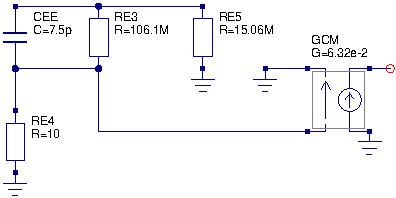
\includegraphics[width=0.8\linewidth]{opamp_fig55}
% tcomb1.png: 99.9998dpi, width=11.35cm, height=3.35cm, bb=0 0 447 132 
  \caption{AC CMRR modification for Boyle macromodel} 
  \label{fig:opamp55}
\end{figure}

\begin{figure} 
  \centering
  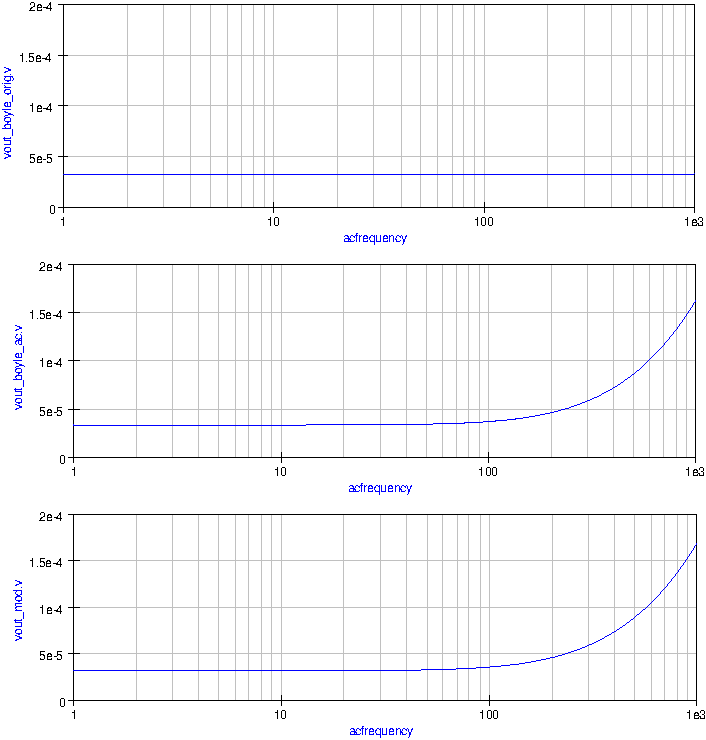
\includegraphics[width=0.8\linewidth]{opamp_fig56}
% tcomb1.png: 99.9998dpi, width=11.35cm, height=3.35cm, bb=0 0 447 132 
  \caption{AC common-mode simulation results for (1) Boyle macromodel, (2) ac Boyle macromodel and (3) the modular macromodel} 
  \label{fig:opamp56}
\end{figure}

\medskip 

Modifying the circuit of an existing OP AMP macromodel is at best a complex process or at worst impossible because the model details are either not known or well understood. One way to add features to an existing model is to add an external circuit to a model's terminals.  This circuit acts as a signal processing element adding additional capabilities to the original macromodel. One circuit feature not modelled by any of the macromodels introduced in earlier sections is power supply rejection. By adding a simple passive electrical network to the terminals of a macromodel it is possible to model OP AMP power supply rejection.  Power supply rejection(PSRR) is a measure of the ability of an OP AMP to reject unwanted signals that enter at the power terminals. It is defined as the ratio of differential-mode gain to power supply injected signal gain. The simulation of OP AMP power supply rejection\footnote{M. E. Brinson and D. J. Faulkner, Measurement and modelling of operational amplifier power supply rejection, Int. J. Electronics, 1995, vol. 78, NO. 4, 667-678.} is possible using the test circuit given in Fig.~\ref{fig:opamp57}, where

\medskip 
$V_{out}(f)^{\pm}=A_{D}(f)\left[ V^{+} - V^{-}\right] +A_{CM}(f)\left[ \dfrac{V^{+} + V^{-}}{2}\right] +A_{PS}(f)^{\pm}V_{S} $,

\medskip 
where $A_{D}(f)$ is the OP AMP differential-mode gain, $A_{CM}(f)$ is the OP AMP common-mode gain, and $A_{PS}(f)^{\pm}$ is the OP AMP power supply injected gain.  The superscript $\pm$ indicates that the ac signal source is connected to either the OP AMP positive or negative power supply terminals but not simultaneously to both.  Assuming that the OP AMP power supply injected gain has a single dominant zero at $f_{PSZ1}^{\pm}$, analysis yields

\bigskip 

$\dfrac{V_{OUT}(f)^{\pm}}{V_{S}}=\dfrac{\dfrac{1}{\alpha P_{SRR}(0)^{\pm}} \left[ 1+j\left( \dfrac{f}{f_{PSZ1}^{\pm}}  \right) \right] }                  {\left[ 1+j\left( \dfrac{f}{\alpha GBP} \right) \right] }$

\bigskip 

Where  $APS(f)^{\pm}=APS(0)^{\pm} \dfrac{\left[ 1+j\left( \dfrac{f}{f_{PSZ1}^{\pm}}\right) \right] }{\left[ 1+j\left( \dfrac{f}{f_{p1}}\right) \right] } $ ,  $\alpha=\dfrac{R2}{R1+R2} = 1e-4$


$PSRR(f)^{\pm} = \dfrac{PSRR(0)^{\pm}}   {\left[ 1+j\left( \dfrac{f}{f_{PSZ1}^{\pm}} \right) \right]}$, $PSRR(0)^{+}=\dfrac{A_{D}(0)}{A_{PS}(0)^{+}}$ and $PSRR(0)^{-}=\dfrac{A_{D}(0)}{A_{PS}(0)^{-}}$.

Typical values for the UA741 are $PSRR(0)^{+}=110000, PSRR(0)^{-}=170000,    f_{PSZ1}^{+}=685Hz, f_{PSZ1}^{-}=6.2Hz$.
\begin{figure} 
  \centering 
  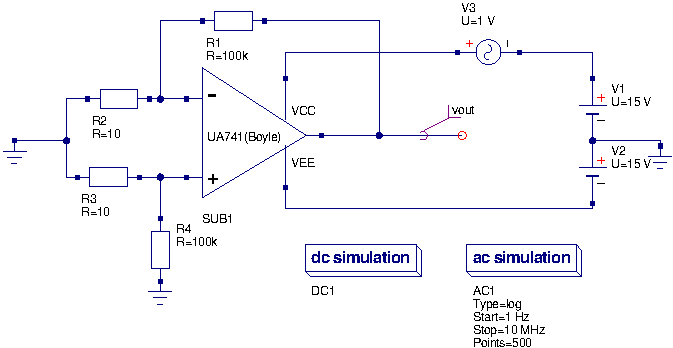
\includegraphics[width=0.8\linewidth]{opamp_fig57}
% tcomb1.png: 99.9998dpi, width=11.35cm, height=3.35cm, bb=0 0 447 132 
  \caption{Test circuit for the simulation of PSRR(f) voltage transfer function characteristic}  
  \label{fig:opamp57}
\end{figure}
The considerable difference in the dominant zero frequencies of the  injected power supply gains is normally due to the fact that the OP AMP circuits are not symmetric when viewed from the power supply signal injection terminals. 
By adding external components to an OP AMP macromodel power supply rejection effects can be easily simulated.  The schematic shown in Fig.~\ref{fig:opamp58} shows the TI UA741 model with RC networks connected between the power supply terminals and earth.  The voltage controlled voltage sources probe the voltages at the center nodes of the additional RC networks.  These networks generate the power supply injected signals at dc. They also generate the dominant zero in the power supply rejection characteristic.  
\begin{flushleft}
The values for the passive components can be calculated using:                                                                               \end{flushleft}
$RA=\dfrac{10^{6}}{PSRR(0)^{+}}$, $CA=\dfrac{1}{2 \cdot 10^{6} \cdot \pi \cdot f_{PSZ1}^{+}}$, $RB=\dfrac{10^{6}}{PSRR(0)^{-}}$, $CA=\dfrac{1}{2 \cdot 10^{6} \cdot \pi \cdot f_{PSZ1}^{-}}$

\bigskip
Which gives, for the example UA741 device data, $RA=9\Omega$, $CA=232pF$, $RB=5.9\Omega$ and $CB=25.7pF$.
Simulation waveforms for the small signal frequency response of the test circuit are shown in Fig.~\ref{fig:opamp59}.  In the case of the modular UA741 model the simulation signal plot clearly demonstrates the fact that the model does not correctly represent the effects due to power supply injected signals. 

\begin{figure} 
  \centering 
  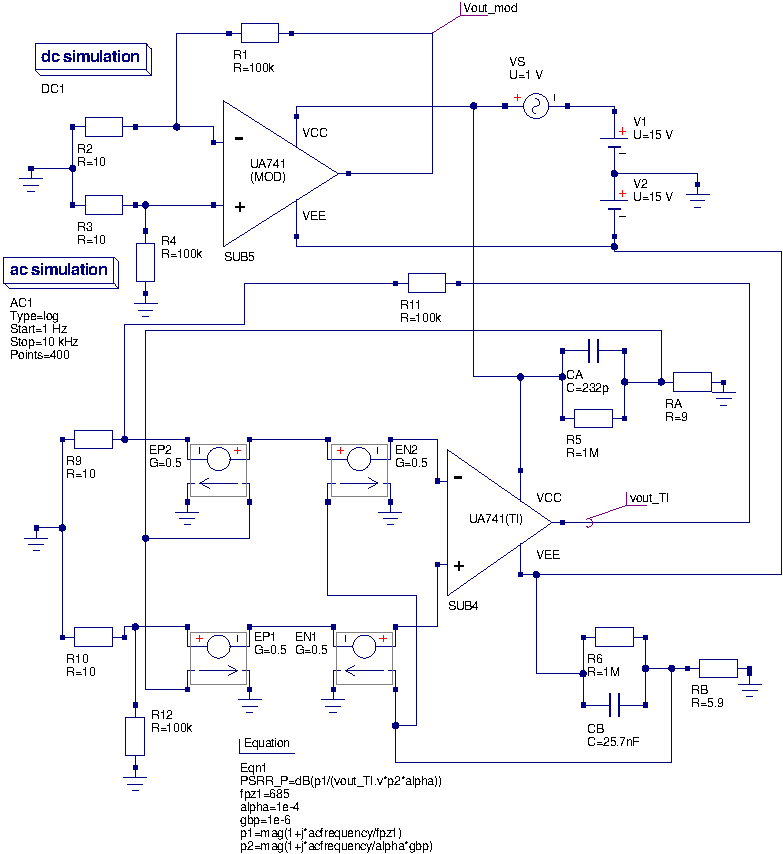
\includegraphics[width=0.8\linewidth]{opamp_fig58}
% tcomb1.png: 99.9998dpi, width=11.35cm, height=3.35cm, bb=0 0 447 132 
  \caption{Test circuit showing OP AMP with external power supply rejection modelling network}   
  \label{fig:opamp58}
\end{figure}

\begin{figure} 
  \centering 
  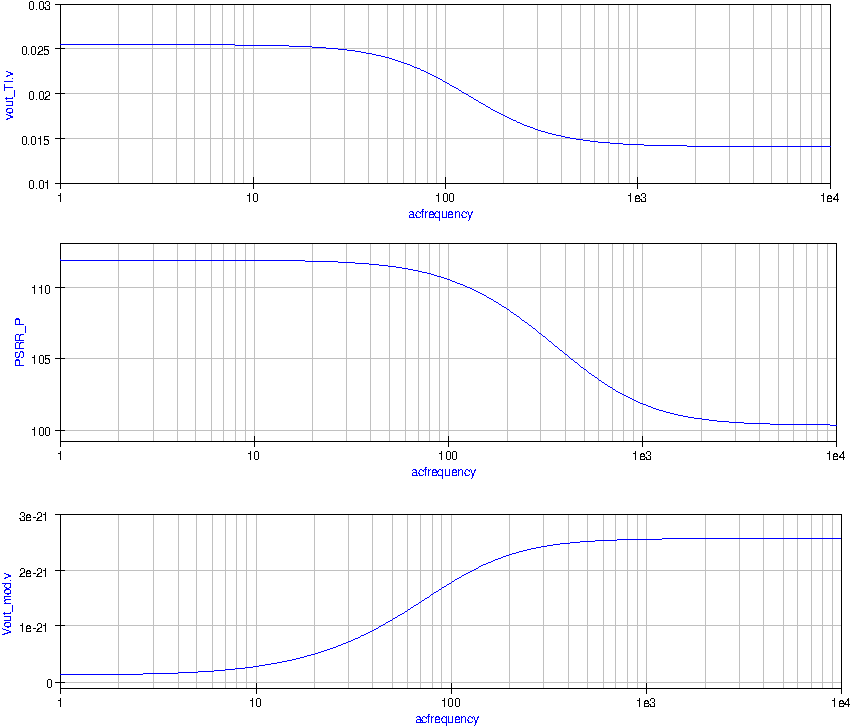
\includegraphics[width=0.8\linewidth]{opamp_fig59}
% tcomb1.png: 99.9998dpi, width=11.35cm, height=3.35cm, bb=0 0 447 132 
  \caption{Simulation waveforms for the circuit illustrated in Fig.~\ref{fig:opamp58}}  
  \label{fig:opamp59}
\end{figure}







\tutsection{End note}
While writing this tutorial I have tried to demonstrate how practical models of operational amplifiers can be constructed using basic electronic concepts and the range of Qucs built-in components.  The modular OP AMP macromodel was deliberately chosen as the foundation for the tutorial for two reasons; firstly Qucs is mature enough to easily simulate such models, and secondly the parameters which determine the operation of the macromodel can be be calculated directly from information provided on device data sheets. Recent modelling development by the Qucs team has concentrated on improving the SPICE to Qucs conversion facilities. This work has had a direct impact on Qucs ability to import and simulate manufacturers OP AMP models. The tutorial upgrade explains how SPICE Boyle type OP AMP macromodels can be converted to work with Qucs. The Qucs OP AMP library (OpAmps) has been extended to include models for a range of popular 8 pin DIL devices. If you require a model with a specific specification that is not modelled by an available macromodel then adding extra functionality may be the only way forward.  Two procedures for extending models are outlined in the tutorial upgrade. Much work still remains to be done before Qucs can simulate a wide range of the macromodels published by device manufacturers.  With the recent addition of subcircuit/component equations to Qucs it is now possible to write generalised macromodel macros for OP AMPs.  However, before this can be done time is required to fully test the features that Stefan and Michael have recently added to Qucs release 0.0.11. This topic and the modelling of other OP AMP properties such as noise will be the subject of a further OP AMP tutorial update sometime in the future.  My thanks to David Faulkner for all his help and support during the period we were working on a number of the concepts that form part of the basis of this tutorial. Once again a special thanks to Michael Margraf and Stefan Jahn for all their help and encouragement over the period that I have been writing this tutorial and testing the many examples it includes.